\documentclass[12pt]{book}
\usepackage[a4paper,
            bindingoffset=0.2in,
            left=1in,
            right=1in,
            top=1in,
            bottom=1.2in,
            footskip=.5in]{geometry}


\usepackage{lipsum}
\usepackage[toc,page]{appendix}
\usepackage{afterpage}
\usepackage{bm}
\usepackage{graphicx}
\usepackage[labelfont=bf]{caption}
\usepackage{amssymb}
\usepackage{amsmath}
\usepackage{svg}
\usepackage{amsfonts}
\usepackage{subcaption}
\usepackage{color,soul}
\usepackage{rotating}
\usepackage{multirow}
\usepackage{siunitx}
\usepackage{hyperref}
\sisetup{scientific-notation=true, output-exponent-marker=\ensuremath{\mathrm{E}}}

\newcommand\blankpage{%
    \null
    \thispagestyle{empty}%
    \newpage}

\usepackage{fancyhdr}
\pagestyle{fancy}
\fancyhf{}
\fancyhead[EL]{\nouppercase\leftmark}
\fancyhead[OR]{\nouppercase\rightmark}
\fancyhead[ER,OL]{\thepage}
\setlength{\headheight}{15pt}% ...at least 51.60004pt

\geometry{
    hmargin={1in, 1in},
    vmargin={1.1in, 1.1in}
} 
\setlength{\headsep}{0.3in}
\savegeometry{origin}

\geometry{
    hmargin={2cm, 2cm},
    vmargin={5cm, 2cm}
} \savegeometry{coverpage}

\usepackage{biblatex}
\addbibresource{bibliography/bibliography.bib}

\usepackage{amsmath}
% \usepackage{acronym}
\usepackage{acro}
\usepackage{xcolor}
\usepackage[ruled]{algorithm2e}

% Define a new command let Stefano insert his comments
\newcommand{\stext}[1]{\color{teal}\rule{\linewidth}{1mm}
{#1}\\
\rule{\linewidth}{1mm}
\color{black}}

% list of acronyms
\DeclareAcronym{adas}{
    short = ADAS,
    long = Advanced Driver Assistance Systems
}
\DeclareAcronym{cagr}{
    short = CAGR,
    long = Compound Annual Growth Rate
}
\DeclareAcronym{oems}{
    short = OEMs,
    long = Original Equipment Manufacturers
}
\DeclareAcronym{acc}{
    short = ACC,
    long = Adaptive Cruise Control
}
\DeclareAcronym{lka}{
    short = LKA,
    long = Lane Keeping Assistance
}
\DeclareAcronym{ldw}{
    short = LDW,
    long = Lane Departure Warning
}
\DeclareAcronym{aeb}{
    short = AEB,
    long = Automatic Emergency Braking
}
\DeclareAcronym{bsd}{
    short = BSD,
    long = Blind Spot Detection
}
\DeclareAcronym{tsr}{
    short = TSR,
    long = Traffic Sign Recognition
}
\DeclareAcronym{dms}{
    short = DMS,
    long = Driver Monitoring System
}
\DeclareAcronym{mpl}{
    short = MPL,
    long = Meta Pseudo Labels
}
\DeclareAcronym{vit}{
    short = ViT,
    long = Vision Transformer
}
\DeclareAcronym{cnn}{
    short = CNN,
    long = Convolutional Neural Network
}
\DeclareAcronym{rnn}{
    short = RNN,
    long = Recurrent Neural Network
}
\DeclareAcronym{lstm}{
    short = LSTM,
    long = Long Short-Term Memory
}
\DeclareAcronym{gru}{
    short = GRU,
    long = Gated Recurrent Unit
}
\DeclareAcronym{mlp}{
    short = MLP,
    long = Multi-Layer Perceptron
}
\DeclareAcronym{vad}{
    short = VAD,
    long = Video Anomaly Detection
}
\DeclareAcronym{var}{
    short = VAR,
    long = Video Action Recognition
}
\DeclareAcronym{convae}{
    short = ConvAE,
    long = Convolutional Autoencoder
}
\DeclareAcronym{convlstmae}{
    short = ConvLSTM-AE,
    long = Convolutional LSTM Autoencoder
}
\DeclareAcronym{sift}{
    short = SIFT,
    long = Scale-Invariant Feature Transform
}
\DeclareAcronym{ransac}{
    short = RANSAC,
    long = Random Sample Consensus
}
\DeclareAcronym{asift}{
    short = ASIFT,
    long = Affine Scale-Invariant Feature Transform
}
\DeclareAcronym{surf}{
    short = SURF,
    long = Speeded-Up Robust Features
}
\DeclareAcronym{mcc}{
    short = MCC,
    long = Matthews Correlation Coefficient
}
\DeclareAcronym{auc}{
    short = AUC,
    long = Area Under the Curve
}
\DeclareAcronym{roc}{
    short = ROC,
    long = Receiver Operating Characteristic
}
\DeclareAcronym{fpr}{
    short = FPR,
    long = False Positive Rate
}
\DeclareAcronym{tpr}{
    short = TPR,
    long = True Positive Rate
}
\DeclareAcronym{pdf}{
    short = p.d.f.,
    long = Probability Density Function
}
\DeclareAcronym{cdf}{
    short = CDF,
    long = Cumulative Density Function
}
\DeclareAcronym{gan}{
    short = GAN,
    long = Generative Adversarial Network
}


\begin{document}
\pagenumbering{roman}
\loadgeometry{coverpage}

% %
\newpage
\stext{Provo ad inserire i commenti in questo modo. Se non ci capiamo cambiamo metodo.}
\stext{Forse hai visto anche che in main.tex ho aggiunto un pacchetto per gestire gli acronimi. L'ho usato per ADAS.
Prova a guardarlo, dovrebbe aiutarti a tenere traccia dell'uso degli acronimi e a mantenere la notazione coerente.}
\stext{Qui inserirei una sezione all'interno del capitolo che racconti qualcosa degli ADAS.
Ti ho incollato qualcosa da ChatGPT, non è completo e ci sono diversi errori, ma credo renda l'idea.
Oltre a questo forse inserirei un preambolo e cercherei di introdurre il problema specifico a cui ti sei approcciato.
Al momento la descrizione del problema è molto generica, ma serve entrare nel dettaglio, soprattutto per dare l'idea
di quali siano i tuoi contributi.\\
Forse avevi già in mente di farlo, ma non hai ancora avuto tempo di scrivere.
Volendo potresti inserire in ogni capitolo un commento (o già una specie di scaletta usando le sessioni, o un mix) 
per chiarire il più possibile il filo logico che vuoi andare a seguire.}
\newpage

\begin{titlepage}
\begin{center}

\vspace*{1cm}
\textbf{\Large{Computer Vision-Based Dangerous Scenes Detection}\\ 
        \vspace*{0.2cm}
        \Large{System for Advanced Driving Assistance}}\\
\vspace*{2cm}
\textbf{\large{Alberto Trabcchin}}\\
\vfill

\vspace*{4cm}
Advisors \\
\vspace*{1cm}
\begin{minipage}[t]{0.48\textwidth}
    Prof. Dr. Yasutaka Fujimoto \\
    Department of Electrical Engineering\\
    Yokohama National University \\
    Japan

\end{minipage}
\hfill
\begin{minipage}[t]{0.48\textwidth}
\begin{flushright}
    Prof. Dr. Monica Reggiani \\
    Department of Management Engineering \\
    University of Padova \\
    Italy
\end{flushright}
\end{minipage}

\vfill

Master Thesis\\
    
\vspace{0.8cm}

    
Department of Electrical and Computer Engineering\\
Yokohama National University\\
Japan\\
September 15, 2024
            
\end{center}
\end{titlepage}

\afterpage{\blankpage}
\loadgeometry{origin}
\thispagestyle{empty}
\section*{Acknowledgements}
\vspace{0.5cm}
I am deeply grateful for the opportunity to conduct my research in the laboratory 
of Professor Yasutaka Fujimoto as part of a double-degree program. This experience 
has been profoundly enriching both personally and professionally. I would like 
to express my heartfelt thanks to the Professor for welcoming me into his laboratory and 
giving me the chance to meet and work with inspirational individuals, including 
Flavis, Besong, Brice, and Martin. Our spontaneous conversations about research 
and our futures were both enjoyable and enlightening.

Morning coffee talks with Eriko Hino were a wonderful way to start each day with 
her positive humor. I also appreciate the effort she puts in as the secretary of 
the laboratory.

My gratitude extends to Professor Roberto Oboe for coordinating this experience 
abroad and connecting me with the laboratory.

Inoue and Ushiyama were instrumental in helping me navigate a culture so different 
from my own. Their assistance made my transition much smoother.

I am profoundly grateful to Professor Monica Reggiani and her group, including 
Professor Stefano Michieletto, for their technical and moral support during 
challenging times in my research.

Special thanks to Elaine, Prateek, and Hassan for their support from the company 
side during my thesis.

I am profoundly thankful to my family and my girlfriend, Giulia, who played a 
key role in this journey. Their unwavering support from day one has been indispensable.

Weekends spent having insightful talks with Marco on our shared interests were 
incredibly motivating. Also your support during difficult times helped me stay 
focused on my goals.

Lastly, but not least, I thank all the other new friends I made in Japan. Your 
presence and support have made this experience unforgettable.
\afterpage{\blankpage}
\thispagestyle{empty}
\section*{Abstract}
\vspace{0.5cm}
This thesis presents a comprehensive study on the development of a computer 
vision-based system for \acf{adas}. The research 
initially explored a classical computer vision approach, which involved 
employing detection and tracking algorithms and monocular depth estimation
to perceive the external environment. Moreover, the study focused on 
integrating the driver’s attention state through its gaze projected from a pair 
of eye-tracking glasses onto the external scene, through a roof-mounted camera.
The primary objective was to analyze the driver's behavior by comparing 
its gaze with the locations of vulnerable road users, thereby proposing 
an initial safety scheme.

Despite the promising conceptual framework, it was observed that many of the 
conventional methods for extracting indirect features were not sufficiently 
robust in real-world driving scenarios. These methods struggled particularly 
under varying light conditions and during critical situations, highlighting 
significant limitations. In response to these challenges, the research 
transitioned to a deep learning-based approach. The core investigation centered 
on the capabilities of a \acf{vit} in extracting human decision-making 
biases inherent in detecting dangerous driving situations.
This approach was further improved by 
employing semi-supervised learning techniques, which leverage the 
vast amounts of easily accessible unlabeled data, thus 
addressing the challenges associated with the expensive and labor-intensive 
labeling process.

The outcomes of this research shows the substantial potential of 
the attention mechanism, on which vision transformer is based, in enhancing 
the robustness 
and reliability of \acs{adas}. The study also opens up new themes for future 
research by identifying and addressing the challenges encountered during the 
development process. These findings underscore the critical role of computer 
vision in the advancement of \acs{adas}, emphasizing its significance in improving 
driver assistance systems through more accurate and reliable perception 
mechanisms.

In conclusion, this thesis contributes to the field of ADAS by demonstrating 
how modern computer vision techniques can be effectively integrated into driver 
assistance systems. It highlights the potential of deep 
learning, especially in overcoming the limitations of traditional methods, and 
points to future innovations for safer and more 
efficient driving experiences.

\afterpage{\blankpage}

\tableofcontents
\listoffigures
\listoftables
\printacronyms
\chapter{Introduction}
\pagenumbering{arabic}

\section{\acl{adas}}
Advanced Driver Assistance Systems (ADAS) are technologies that improve road 
safety by enhancing both vehicle and driver capabilities. These systems support 
the driver in the driving process, reducing the likelihood of human error and 
increasing road safety. ADAS includes a range of features from basic functions 
such as automatic headlights and rain-sensing windshield wipers to more complex 
systems like adaptive cruise control, lane departure warning, and collision 
avoidance systems.

The evolution of ADAS has been fueled by advancements in sensors, computing 
power, and connectivity. These technologies work together to provide vehicles 
with the ability to not only sense their environment but also to analyze and 
respond to potential hazards. As such, ADAS is seen as a crucial step towards 
fully autonomous vehicles, providing a safer, more comfortable driving experience.

\subsection{Market Size and Growth}
The market for \ac{adas} is experiencing robust growth as these technologies 
become more integral to new vehicle designs, emphasizing safety and driving 
efficiency. 

In 2024, the global ADAS market is projected to be worth around 
\$64.05 billion, with expectations to expand significantly at a \ac{cagr} 
of 12.7\% reaching approximately \$211.71 billion by 2034 \cite{adas_report_2023}.
This growth is given by advancements in autonomous driving technology and 
an increasing emphasis on vehicle safety from both consumers and functional 
safety certifications. 
Significant investments are also being made in the development and 
implementation of ADAS technologies across various global markets, including 
Japan, China, the United States, and Europe \cite{adas_report_2023}.

\begin{table}[h]
    \centering
    \begin{tabular}{r|c}
        \hline
        \textbf{Market} & \textbf{CAGR} \\
        \hline
        Worldwide & 12.7\% \\
        Japan & 13.6\% \\
        China & 13.5\% \\
        United States & 12.5\% \\
        Canada & 9.7\% \\
        Germany & 8.8\% \\
        Spain & 8.5\% \\
        \hline
    \end{tabular}
    \caption{\ac{cagr} of the ADAS market in different countries \cite{adas_report_2023}.}
    \label{tab:adas_revenue}
\end{table}
Considering the market value and growth rate of \ac{adas} technologies, 
ADAS systems must also be economically viable on a large scale. 
This necessitates the use of cost-effective sensors such as cameras and radars, 
which offer a balance between performance and affordability. While there are 
more accurate options available, such as LiDAR sensors, these are typically more 
expensive and are primarily used for self-driving car experiments in research 
laboratories. The high cost of LiDAR sensors makes them less suitable for 
widespread deployment in consumer vehicles. Therefore, the challenge lies in 
leveraging affordable technologies like cameras and radars to their maximum 
potential, to deliver effective ADAS systems that can be widely adopted.

\subsection{Market Ecosystem}
The market ecosystem for \ac{adas} can be 
conceptually divided into several layers, each representing a different segment 
of the value chain. These layers range from \ac*{oems} to the suppliers of the key 
components such as sensors and processors. 
Here's a breakdown of these layers and the main companies in each field:

\subsubsection{\ac{oems}}
\acl{oems} are companies that integrate ADAS into their vehicles. They either develop 
some of their own ADAS technologies or incorporate systems designed by 
Tier 1 suppliers. Some of the leading OEMs in the ADAS market include 
Honda, Toyota, Nissan, General Motors, Tesla, Ford, Volkswagen, Volvo, BMW, and 
Mercedes-Benz.

\subsubsection{Tier 1 Suppliers}
Tier 1 suppliers develop complete systems or significant components that are 
directly supplied to \ac{oems}. These companies often develop the software and 
hardware integration necessary for ADAS.
Main Tier 1 suppliers in the ADAS market include Bosch, Continental, Aptiv, 
Denso, Magna, and Valeo.

\subsubsection{Autonomous Technology Developers}
This layer includes companies specifically focused on developing software and 
platforms that enable autonomous driving capabilities beyond standard ADAS features.
Key players in this segment include Waymo (Google/Alphabet), Cruise (General Motors),
Argo AI (Ford, Volkswagen), Aurora, and Zoox (Amazon).

\subsubsection{Sensing and Perception}
Companies in this segment focus on developing sensors and perception technologies 
that allow vehicles to perceive their environment, which is essential for both 
ADAS and fully autonomous functionalities.
Main providers are Luminar (LiDARs), Velodyne (LiDARs), Mobileye (cameras), 
Foresight Autonomous (cameras).

\subsubsection{Processors and Computing}
This segment involves the manufacturers of the advanced computing systems that 
process inputs from various sensors to make real-time driving decisions.
Key players include NVIDIA (GPUs and SoCs), Intel (through Mobileye), 
Qualcomm (processors), NXP Semiconductors (microcontrollers), and 
Renesas (microcontrollers and SoCs).

\subsubsection{Sensors}
This layer includes manufacturers of the various types of sensors used in ADAS 
and autonomous vehicles, such as cameras, radar, LiDAR, and ultrasonic sensors.
Main companies in this segment include Bosch (radar and video sensors),
Continental (radar sensors), Sony (image sensors), Texas Instruments (radar chips),
and ON Semiconductor (image sensors for automotive cameras).


\subsection{Key Components of \ac{adas}}
\ac{adas} systems are composed of several key components that work together to 
enhance vehicle safety and driving experience. These components include sensors, 
control units, actuators, human-machine interface, and connectivity.

\subsubsection{Sensors}
Sensors help the vehicle perceive its environment by collecting data on the 
surrounding objects and road conditions. The main types of sensors used in ADAS 
systems are:

\begin{itemize}
    \item \textbf{Radar Sensors}: These sensors use radio waves to detect the 
    distance and speed of objects around the vehicle. They are particularly 
    useful for measuring the relative speed of other vehicles and detecting 
    objects in poor weather conditions.
    
    \item \textbf{Cameras}: Cameras provide visual data that is used for object 
    recognition, lane detection, traffic sign recognition, and other visual 
    tasks. They are essential for understanding the vehicle's surroundings and 
    identifying potential hazards.
    
    \item \textbf{Ultrasonic Sensors}: These sensors are used for close-range 
    detection, primarily in parking assistance systems. They help the vehicle 
    detect obstacles when maneuvering at low speeds.
    
    \item \textbf{LiDAR}: LiDAR sensors use laser pulses to create a 3D map of 
    the vehicle's surroundings. They are particularly useful for creating 
    detailed maps of the environment and detecting objects at longer ranges.
\end{itemize}

\subsubsection{Control Units}
Control units are responsible for processing the data from sensors and cameras, 
making real-time decisions, and sending commands to the vehicle's actuators.
Decision making algorithms are implemented in these units to interpret sensor 
data and determine the appropriate response to different driving scenarios.

\subsubsection{Actuators}
Actuators are the components that control the vehicle's braking, steering, and 
acceleration systems based on the commands received from the control units. 
These actuators are responsible for executing the decisions made by the ADAS 
to ensure safe and efficient driving.

\subsubsection{Human-Machine Interface}
The human-machine interface is the system through which the driver interacts 
with the ADAS. This interface includes displays, alerts, and notifications that 
inform the driver about the status of the vehicle and provide warnings or 
assistance when needed. The interface is crucial for ensuring that the driver 
remains aware of the vehicle's behavior and can intervene when necessary.

\subsubsection{Connectivity}
Connectivity is an essential component of modern ADAS systems, enabling 
communication between the vehicle and external systems. This connectivity allows 
the vehicle to receive real-time traffic information, software updates, and 
remote assistance. It also enables vehicle-to-vehicle and vehicle-to-infrastructure 
communication, which is crucial for advanced safety features like collision 
avoidance and traffic management.


\subsection{Common \ac{adas} Features}
ADAS systems offer a wide range of features that enhance vehicle safety, 
comfort, and efficiency. Some of the most common ADAS features include: 
\ac*{acc}, \ac*{ldw}, \ac*{bsd}, \ac*{aeb}, \ac*{tsr}, \ac*{dms}, parking assistance,
adaptive headlights, and more. Most important functionalities are described in detail.

\subsubsection{\ac{acc}}
\ac{acc} is a feature that maintains a set speed and adjusts it to keep a safe 
distance from the vehicle ahead. It uses sensors to detect the distance and 
speed of the vehicle in front and automatically adjusts the vehicle's speed to
maintain a safe following distance.

\subsubsection{\ac{ldw}}
\ac{ldw} is a system that alerts the driver if the vehicle begins to drift out 
of its lane without signaling. It uses cameras or sensors to monitor the vehicle's 
position within the lane and provides visual or audible warnings if the vehicle 
starts to veer off course. Some vehicles also have \ac{lka} systems that can 
automatically steer the vehicle back into its lane if the driver does not respond 
to the warnings.

\subsubsection{\ac{bsd}}
\ac{bsd} is a system that warns the driver of vehicles in the blind spot during
lane changes. It uses sensors to detect vehicles in adjacent lanes that may not
be visible in the side mirrors and provides visual or audible alerts to prevent
collisions during lane changes.

\subsubsection{\ac{aeb}}
\ac{aeb} is a safety feature that detects imminent collisions with vehicles,
pedestrians, or other obstacles and automatically applies the brakes to prevent
or mitigate the impact. This system helps reduce the severity of accidents by
providing an additional layer of protection when the driver fails to react in
time.

\subsubsection{\ac{tsr}}
\ac{tsr} is a feature that uses cameras or sensors to identify traffic signs
such as speed limits, stop signs, and road markings. It displays this information
on the vehicle's dashboard or head-up display, helping the driver stay informed
about the current road conditions and regulations.

\subsubsection{\ac{dms}}
\ac{dms} is a system that monitors the driver's attention and alertness while
driving. It uses sensors to track the driver's eye movements, head position, and
other behavioral cues to detect signs of drowsiness, distraction, or inattention.
The system can provide warnings or take corrective actions to prevent accidents
caused by driver fatigue or distraction.



% Sample text
%%%%%%%%%%%%%%%%%%%%%%%%%%%%%%%%%%%%%%%%%%%%%%%%%%%%%%%%%%%%%%%%%%%%%%%%%%%%%%%%
% \section{\acl{adas}}
% %
% \ac{adas} are electronic systems in vehicles that use advanced technologies to assist the driver in the driving process. 
% These systems enhance vehicle safety and facilitate safer and more efficient driving by providing real-time information, automation, and alerts. 
% Here's an overview of the key components and functionalities of \ac{adas}:
% %
% \subsection*{Key Components of \ac{adas}}
% \begin{itemize}
%     \item \textbf{Sensors and Cameras}:
%     \begin{itemize}
%         \item \textit{Radar Sensors}: Measure the distance and speed of objects around the vehicle.
%         \item \textit{Cameras}: Provide visual data for object recognition, lane detection, and traffic sign recognition.
%         \item \textit{Ultrasonic Sensors}: Used for close-range detection, primarily in parking assistance.
%         \item \textit{Lidar}: Uses laser pulses to create a 3D map of the vehicle's surroundings.
%     \end{itemize}
    
%     \item \textbf{Control Units}:
%     \begin{itemize}
%         \item \textit{Electronic Control Units (ECUs)}: Process data from sensors and cameras, making real-time decisions and sending commands to actuators.
%     \end{itemize}
    
%     \item \textbf{Actuators}:
%     \begin{itemize}
%         \item Control the vehicle's braking, steering, and acceleration systems based on commands from the control units.
%     \end{itemize}
% \end{itemize}
% %
% \subsection*{Common \ac{adas} Features}
% \begin{itemize}
%     \item \textbf{Adaptive Cruise Control (ACC)}:
%     Maintains a set speed and adjusts it to keep a safe distance from the vehicle ahead.
%     \item \textbf{Lane Departure Warning (LDW) and Lane Keeping Assist (LKA)}:
%     \begin{itemize}
%         \item \textit{LDW}: Alerts the driver if the vehicle begins to drift out of its lane.
%         \item \textit{LKA}: Gently steers the vehicle back into its lane if it starts to drift.
%     \end{itemize}
%     \item \textbf{Blind Spot Detection (BSD)}:
%     Warns the driver of vehicles in the blind spot during lane changes.
%     \item \textbf{Automatic Emergency Braking (AEB)}:
%     Detects imminent collisions and applies the brakes automatically if the driver does not respond in time.
%     \item \textbf{Traffic Sign Recognition (TSR)}:
%     Identifies traffic signs and displays them on the dashboard or head-up display.
%     \item \textbf{Driver Monitoring Systems (DMS)}:
%     Monitors the driver’s attention and alertness, providing warnings or taking action if signs of drowsiness or distraction are detected.
%     \item \textbf{Parking Assistance}:
%     Includes features like rearview cameras, parking sensors, and automatic parking systems that assist with parking maneuvers.
%     \item \textbf{Night Vision Enhancement}:
%     Uses infrared sensors to detect objects and pedestrians in low-light conditions, displaying this information to the driver.
% \end{itemize}
% %
% \subsection*{Benefits of \ac{adas}}
% \begin{itemize}
%     \item \textbf{Safety}: Reduces the likelihood of accidents by providing warnings and taking proactive actions.
%     \item \textbf{Comfort}: Reduces driver workload by automating repetitive tasks like cruising and parking.
%     \item \textbf{Efficiency}: Helps in maintaining optimal driving patterns, potentially reducing fuel consumption.
%     \item \textbf{Regulatory Compliance}: Meets safety standards and regulations imposed by automotive safety authorities.
% \end{itemize}
% %
% \subsection*{Future of \ac{adas}}
% As technology advances, \ac{adas} is expected to evolve toward higher levels of automation, ultimately contributing to fully autonomous driving. Enhanced connectivity, improved sensor technology, and advanced artificial intelligence will continue to drive innovations in this field.
% %
%%%%%%%%%%%%%%%%%%%%%%%%%%%%%%%%%%%%%%%%%%%%%%%%%%%%%%%%%%%%%%%%%%%%%%%%%%%%%%%%




\section{Focus of this work}
%
In the field of modern automotive technology, \ac{adas} are playing a keyrole at augmenting driver safety, comfort, and overall driving experience.
These systems, leveraging advancements in computer vision, sensor technologies, and artificial intelligence, are reshaping the automotive industry introducing semi-autonomous and autonomous driving capabilities.

According to the \ac{who} road traffic injuries are among the leading causes of death worldwide, with an estimated 1.19 million fatalities annually.
With the aim of contributing to this transformative field, in this thesis various computer vision algorithms are implemented and evaluated, analyzing their strengths and weaknesses in addressing specific driving tasks.
From tracking of vulnerable users, such as pedestrians and cyclists, to the comprehension of dynamic driving environments, this research highlights advantages and limitations of each approach in real-world scenarios.
Further considerations are made on the trade-offs between complexity of the tasks and available data to train the models. 

By scrutinizing the performance of these algorithms in real-world scenarios and carefully assessing their respective advantages and limitations, this thesis aims to provide valuable insights into their applicability and efficacy within the domain of \ac{adas}. 
Through this rigorous evaluation process, a nuanced understanding of the suitability of different computer vision techniques for specific driving tasks is achieved, paving the way for informed decision-making and future advancements in automotive safety and technology.

In the pursuit of contributing to this transformative field, this thesis endeavors to explore and implement a computer vision-based approach for \ac{adas} systems. 
Specifically, the focus is on devising methodologies to enhance perception and decision-making capabilities within the realm of \ac{adas} through the lens of computer vision.

This thesis is divided into two main approaches, each addressing distinct facets of \ac{adas} functionality.
The first approach revolves around a traditional computer vision methodology, leveraging principles of multiple view geometry and object tracking. 
By harnessing the fundamentals of geometric and visual analysis, this approach aims to provide robust and reliable solutions for tasks such as lane detection, object recognition, and tracking within the \ac{adas} framework.

The second approach represents a departure from conventional techniques, delving into the realm of deep learning and vision transformers. 
Here, the emphasis shifts towards a more generalized approach to video-frame classification, leveraging the power of deep neural networks and semi-supervised learning techniques. 
By harnessing the capacity of vision transformers to capture intricate spatial and temporal features from raw video data, this approach seeks to push the boundaries of \ac{adas} capabilities, particularly in scenarios involving complex and dynamic environments.

Through the amalgamation of these two distinct approaches, this thesis endeavors to contribute to the ongoing evolution of \ac{adas} systems, striving towards the realization of safer, more efficient, and ultimately autonomous driving experiences. 
By exploring the synergy between traditional computer vision methodologies and cutting-edge deep learning techniques, this work aims to unlock new directions for innovation and advancement within the realm of automotive technology.

\section{Thesis Organization}
\lipsum[1-2]

%
\chapter{Related Work}
\label{chpt:related_work}
We review recent work in behavioral intention prediction through standard 
methods, including object detection and tracking, and more advanced deep learning 
techniques. Moreover, we introduce advantages and limitations of some methods 
that are capable to improve scene understanding.

\section{Available Datasets}
Pedestrian detection and tracking are fundamental tasks in the field of computer 
vision applied to advanced driving assistance systems. If this task is innate 
to humans, it is still a challenging problem for machines. In addition to the 
complexity of the task many applications require real-time processing 
constraints which can affect accuracy of results. 

In the computer vision field object detection can be approached through two f
different perspectives. The former is to make predictions on general datasets 
that are used as benchmarks for the community, such as COCO \cite{coco}.
In this case the goal is to develop a vision model capable to detect a wide 
range of objects, in many different scenarios.
The latter is task-specific oriented, where the goal is to detect a relative 
small subset of objects in a specific context. This is the case of pedestrian 
detection in driving scenarios.

Nowadays, in the field of intelligent transportation systems, many datasets 
have been released to accomplish detection of some common objects, including 
pedestrians, cyclists, and different types of vehicles.
The most common used for benchmarking state of the art algorithms are KITTI 
\cite{kitti}, Berkeley DeepDrive \cite{bdd100k}, Waymo Open Dataset 
\cite{waymo} and nuScenes \cite{nuscenes}. Moreover, each of these datasets 
has its own peculiarity, such as the quantity of video recordings, the variety 
of scenarios, the number of annotated objects, and the quality of ground-truth 
targets, that can be manually annotated or automatically generated.

Despite semi-autonomous driving is getting a lot of attention in the last years 
and it is expected to continue to grow, the state of the art algorithms are far 
away from the robustness and reliability that industry requires. Moreover, it 
has been shown that the performance can drastically drop when models are tested 
on different datasets, and some customized evaluation metrics could be required 
depending on the accomplished task \cite{uricar2019challenges}.
Therefore it is fundamental to deserve as much attention to the quantity and quality of the data 
as to model design process.

\section {Multi-Object Tracking}
Multi-object tracking (MOT) aims to estimate bounding boxes of objects and 
associate them an unique ID across multiple time frames. This task is 
fundamental in perception of the environment because human behaviors are often 
time-dependent. For example it is important to predict pedestrians' trajectories 
to avoid collisions or to understand their intentions. Tracking is performed by 
estimating the future position of objects based on their past spatial and 
temporal information.

Object detection and tracking are distinct tasks, yet both are essential for 
the tracking process. Within tracking, there are two main aims: 
\textit{"tracking by detection"} and \textit{"detection by tracking"}. 
The former leverages powerful modern object detectors to increase tracking 
accuracy. Usually only bounding boxes' features are considered for the task.
The latter, on the other hand, aims to imporve tracking accuracy with the help 
of tracking information. After the detection phase, most MOT methods discard 
some bounding boxes depending on a detection threshold 
\cite{retinatrack,transtrack}; 
therefore all objects related to these boxes are lost for the considered time 
frame. There are also other methods, like ByteTrack \cite{bytetrack}, that are 
able to track partially-occluded objects in real-world scenarios with 
real-time performance. 

For example, ByteTrack does not discard all bounding 
boxes below a certain confidence threshold, but it keeps almost every detection 
dividing them into high score ones and low score ones. At first high score 
detection boxes are matched with corresponding tracklets. Then, due to 
occlusions, resizes and motion blur, remaining unmatched tracklets are 
combined with low score detection boxes. 

\section{Image Classification}
Image classification is a fundamental task in computer vision, as it is also 
used in the detection pipeline. In the last years, many models based on 
convolutional neural networks (CNNs) have been proposed, but nowadays research 
is moving towards more complex classfication tasks using different 
architectures.
The most succesful CNN-based models are, in a chronological order, 
AlexNet \cite{alexnet}, 
VGG \cite{vggnet}, Inception \cite{inception}, ResNet \cite{resnet}, 
DenseNet \cite{densenet} and 
EfficientNet \cite{efficientnet}.

AlexNet \cite{alexnet} was among the pioneering models to incorporate deep convolutional 
layers, stacking five layers that increased the parameter count to 60 million. 
Additionally, it implemented several strategies to mitigate overfitting, 
including the application of dropout. 
Then VGG \cite{vggnet} still increased the number of 
convolutional layers to 16, reaching the state of the art in the ImageNet 
dataset \cite{imagenet}. However, its 138 million parameters made it 
computationally expensive.
Inception \cite{inception}, on the other hand, was able to increase 
the accuracy reducing the model size through multi-scale convolution transforms 
with filters of varying sizes. Transformations were applied to input features 
in parallel, and then concatenated to form the output.
Therefore, it was able to capture diverse spatial information reducing the 
model size to 4 million parameters.
Then ResNet \cite{resnet} brought a revolutional change of CNN architectures, introducing 
the concept of \textit{residual learning}. In particular it addressed the 
problem of vanishing and exploding gradients in very deep models by introducing 
skip connections between layers. This allowed to train a 152-layer CNN model 
that outperformed shallower models.
After ResNet, DenseNet \cite{densenet} introduced another novel aspect by fully connecting 
all convolutional layers with each other in a forward way. 
Unlike traditional CNN architectures where layers are connected in a sequential 
manner, DenseNet establishes direct connections between all layers in a 
feed-forward manner. This dense connectivity enhances feature reuse and 
facilitates gradient flow throughout the network, leading to improved 
parameter efficiency and feature propagation. As a result, DenseNet has shown 
significant improvements in performance and efficiency compared to earlier 
architectures.
Finally, EfficientNet \cite{efficientnet} proposed a new scaling method that uniformly scales 
depth, width, and resolution leading to a better performance. It was able to 
achieve state of the art results on ImageNet as well as on CIFAR-100 while 
being 8.4 times smaller and 6.1 times faster on inference than the best models.

Through this section it was possible to compare main improvements between 
different CNN architectures, and to understand how they evolved over time.
However, by their nature, CNNs are design to extract features from images that 
can be associated to specific object patterns. Through some hyperparameters, 
like kernel size, downsampling, and number of layers, they can be adapted to extract 
features at different scales and with different resolutions. Considering scene 
understanding in driving scenarios, it is fundamental to caputre relative and 
absolute spatial relations of sub-areas in the main scene. 
Therefore, to address this problem, it is necessary to mode towards models 
designed with different architectures, capable to include these kind of 
information. One possible solution is using a vision transformer model (ViT)
\cite{vit}, that is based on the transformer architecture 
\cite{attention_is_all_you_need}. It consists of a 
self-attention mechanism that allows to tokenize sub-areas of the image and 
capture their spatial relations. This implies that relations are not just 
limited as local features, like with CNNs, but can be extended to all locations 
in the image through the tokens.

In Table \ref{tab:cnn_comparison} a comparison of the discussed models is 
reported. It is possible to see the trending increase of parameters and 
performance over time, but also how since Inception model size has been reduced 
thanks to the introduction of new techniques. It is also possible to notice 
how vision transformer achieves state of the art results with a large model 
size and computational cost, due to the connections between all tokens for 
the self-attention mechanism.

\begin{table}[ht]
    \centering
    \begin{tabular}{l|c|c|l|l|l|c}
        \hline
        \textbf{Model} & \textbf{top-1 [\%]} & \textbf{top-5 [\%]} & 
        \textbf{Params.} & \textbf{GFLOPS} & \textbf{Size [MB]} & 
        \textbf{Year} \\
        \hline
        \hline
        AlexNet & 56.522 & 79.066 & 61.1M & 0.71 & 233.1 & 2012 \\
        \hline
        VGG11 & 69.020 & 88.628 & 132.9M & 7.61 & 506.8 & 2014 \\
        VGG13 & 69.928 & 89.246 & 133.1M & 11.31 & 507.5 & \\
        VGG16 & 71.592 & 90.382 & 138.4M & 15.47 & 527.8 & \\
        VGG19 & 72.376 & 90.876 & 143.7M & 19.63 & 548.1 & \\
        \hline
        Inception\_v3 & 77.294 & 93.45 & 27.2M & 5.71 & 103.9 & 2014 \\
        \hline
        ResNet18 & 69.758 & 89.078 & 11.7M & 1.81 & 44.7 & 2015 \\
        ResNet34 & 73.314 & 91.420 & 21.8M & 3.66 & 83.3 & \\
        ResNet50 & 76.130 & 92.862 & 25.6M & 4.09 & 97.8 & \\
        ResNet101 & 77.374 & 93.546 & 44.6M & 7.8 & 170.5 & \\
        ResNet152 & 78.312 & 94.046 & 60.2M & 11.51 & 230.4 & \\
        \hline
        DenseNet121 & 74.434 & 91.972 & 7.9M & 2.83 & 30.8 & 2016 \\
        DenseNet161 & 77.138 & 93.560 & 28.7M & 7.73 & 110.4 & \\
        DenseNet169 & 75.600 & 92.806 & 14.2M & 3.36 & 54.7 & \\
        DenseNet201 & 76.896 & 93.370 & 20.1M & 4.29 & 77.4 & \\
        \hline
        Effic.Net\_b0 & 77.692 & 93.532 & 5.3M & 0.39 & 20.5 & 2019 \\
        Effic.Net\_b1 & 78.642 & 94.186 & 7.8M & 0.69 & 30.1 & \\
        Effic.Net\_b2 & 80.608 & 95.310 & 9.2M & 1.09 & 35.2 & \\
        Effic.Net\_b3 & 82.008 & 96.054 & 12.3M & 1.83 & 47.2 & \\
        Effic.Net\_b4 & 83.384 & 96.594 & 19.4M & 4.39 & 74.5 & \\
        Effic.Net\_b5 & 83.444 & 96.628 & 30.4M & 10.27 & 116.9 & \\
        Effic.Net\_b6 & 84.008 & 96.916 & 43.1M & 19.07 & 165.4 & \\
        Effic.Net\_b7 & 84.122 & 96.908 & 66.3M & 37.75 & 254.7 & \\
        \hline
        ViT-b\_16 & 81.072 & 95.318 & 86.6M & 17.56 & 330.3 & 2020 \\
        ViT-b\_32 & 75.912 & 92.466 & 88.3M & 4.41 & 336.6 & \\
        ViT-l\_16 & 79.662 & 94.638 & 304.4M & 61.55 & 1161.0 & \\
        ViT-l\_32 & 76.972 & 93.070 & 306.6M & 15.38 & 1169.4 & \\
        ViT-h\_14 & 88.552 & 98.694 & 633.5M & 1016.72 & 2416.6 & \\
        \hline
    \end{tabular}
    \caption[Comparison of vision models for image classification on ImageNet.]
    {Comparison of vision models for image classification on ImageNet.
    Data are taken from 
    \cites{pytorch_alexnet}{pytorch_vgg}{pytorch_inception_v3}{pytorch_resnet}{densenet}
    {pytorch_efficientnet}{pytorch_vision_transformer}.}
    \label{tab:cnn_comparison}
\end{table}


\section{Video Classification}
Along with image classification, time-series analysis started gaining attention. 
The initial focus was on univariate and multi-variate input 
data not directly related to images. 
The introduction of Recurrent Neural Networks (RNNs) \cite{rnn} marked a 
significant improvement in analyzing this kind of data. Recurrent neural 
network represents the simplest sequential architecture, and its main 
peculiarity is the presence of a feedback loop that allows to save an internal 
state based on information from previous time steps. Then for each current time 
step the input is combined with the internal state.
Despite the potential of RNNs, they are not able to capture long-term 
information from data sequences. This is due to the vanishing and exploding 
gradient problem, when there are many feedback loops in the network, and it is 
similar to the problem described for deep CNNs.

To address this issue, Long Short-Term Memory (LSTM) \cite{lstm} was introduced. 
LSTM is a modified version of RNN capable to capture both long and short-term 
dependencies in data sequences through specific internal gates. 
A further improvement was introduced with Gated Recurrent Units (GRUs) 
\cite{gru}, that are a simplified version of LSTM with fewer gates and 
parameters.

However, with the advent of image classification in computer vision, 
the interest in video analysis rose. Considering the previous work on RNNs, 
it was natural to extend the concept of time-series analysis to video time 
frames combining RNNs with CNNs. This led to the introduction of 3D CNNs that 
are capable to extract spatio-temporal features from video sequences through 
3D convolutional kernels.

As for image classification, recent developments in the field focused on 
transformer-based models. In particular, the recent ViViT model \cite{vivit} 
utilizes a similar concept of 3D CNNs, but applied to the vision transformer. 
The model stacks images of the video sequence and then applies the transformer 
architecture to capture spatio-temporal relations between them. 
While this approach outperforms 3D CNNs in terms of effectiveness, it comes with 
increased computational costs for training.

\section{\acl{vad}}
\ac{vad} is a challenging task that aims to 
identify patterns in data that do not conform to expected results. It is a 
more general task, not only focused in driving scenarios, but also used in 
medical imaging, surveillance systems, and industrial quality control.
However, many of these techniques are cross-domain, meaning they can be applied and 
adapted to various fields beyond their initial area of application.
Generally, the two main aspects to focus on are the availability 
of datasets and the development of effective models. In the following subsections
we will list some of the most common datasets and models used in the field of 
\ac{vad}. We also distinguish training methods, supervised, unsupervised and 
semi-supervised, to accomplish different tasks.

However, \ac{vad} is usually performed in an unsupervised mode due to the 
scarcity of data. Therefore, when necessary, we will also include some works 
related to \ac{var} that can be adapted to \ac{vad}.

\subsection{Existing \acs{vad} Datasets}
Considering the common techniques used in \ac{vad}, and the initial focus 
on surveillance systems, many more datasets have been released in this field 
compared to driving scenarios. Therefore, we divide the datasets into 
two categories: surveillance and driving-related datasets.

\subsubsection*{Surveillance Datasets}
Li et al. proposed UCSD Ped1/Ped2 \cite{ucsd}, 
a dataset of densely 
crowded pedestrian walkways to detect abnormal movements and prohibited objects.
In particular, "Ped1" is based on 70 scenes where peple are walking toward and 
away from the camera.
"Ped2" is composed of 28 scenes depicting pedestrians walking almost 
horizontally to the camera.
Another dataset is Avenue \cite{avenue}, a dataset of 15 sequences with 14 
unusual events, such as throwing objects, running, and loitering, with a total 
of 35,240 frames.
Liu et al. proposed ShanghaiTech \cite{shanghaitech_dataset}, a dataset of 437 
videos (330 
for training and 107 for testing) with 130 abnormal events and a total of 
13 different scenes related to walking pedestrians.
Finally, the UCF-Crime dataset \cite{ucf_crime} is composed of 1900 videos 
with 13 anomalies including robberies, accidents, and thefts.

\subsubsection*{Driving Datasets}
Chan et al. introduced a new dataset with 678 dashcam accident videos taken from 
the web \cite{anticip_accident_dashcam}; in each video, the last 10 frames are 
labelled as anomalous.
Yao et al. proposed AnAn Accident Detection (A3D)\cite{a3d}, which contains 1,500
anomalous driving videos with the start and end frames' annotations. In total 
the dataset contains, respctively, 79,991 and 128,175 training and testing frames.
There are 1,500 anomaly events that include targets like cars, trucks, bikes, 
pedestrians and animals.

Considering the interaction of the driver's gaze towards the environment,
there is Driver Attention Prediction in Driving Accident scenarios (DADA) 
\cite{dada1}, \cite{dada2}, a dataset of 2,000 videos focused on the prediction 
of the driver's gaze in accident scenarios. In total they collected 658,476 
frames, each labelled as normal or anomalous. A similar work was proposed 
by Palazzi et al. with DR(eye)VE \cite{dreyeve}, a dataset based on 74 
videos, 8 drivers, over 500,000 frames, 6 total hours of driving in 
downtowns, countrysides and highways. 
However, DR(eye)VE is focused on prediction of the driver's gaze in 
safe scenarios, not in accident ones.

Xia et al. created the BDD-A \cite{bdd_a} dataset, a subset of the Berkeley 
DeepDrive dataset \cite{bdd100k} with 1,232 critical scenes and a total of 
3.5 hours of driving. To create the dataset, they selected video clips that 
both included braking events and took place in busy areas, and then included 
6.5 seconds before and 3.5 seconds after the braking event.
They also collected gaze data of 45 partecipants, who were asked to watch 
the videos and press a button when they noticed an unsafe maneuver.

Finally, a recent dataset focused on detection of traffic accidents is DoTA 
\cite{dota_dataset}. It contains 4,677 videos with temporal, spatial, and 
categorical annotations. In total there are 9 different categories of accidents,
including collision with other vehicles in different directions and out-of-control 
situations. Moreover, they double the classes, splitting each category to 
ego-involved and non-ego-involved accidents, resulting in 18 categories total.

\subsection{State-of-the-Art \acs{vad} and \acs{var} Models}
\acl{vad} models for driving scenarios can be divide into three main categories, 
depending on the available data and learning approach: 
unsupervised, semi-supervised, and supervised mode.
Typically, it is easy to collect unlabelled data through ego-vehicle-mounted 
cameras or dashcams, while labelled data is much more difficult and expensive 
to obtain. Moreover, the quality of the labels can be affected by human 
subjectivity, age, and experience. Therefore, most of the research in this 
field is focused on unsupervised and semi-supervised learning.

Another imoprtant division is related to what features to extract: some models 
consider a single frame to analyze, while others take a sequence through a 
sliding time window. 

\subsubsection*{Unsupervised Learning}
Hasan et al. \cite{hasan_convae} proposed a \ac{convae} model for reconstructing 
some stacked frames. Then anomalies were identified by comparing the 
reconstruction error. They fonud out that anomalies were better detected with 
longer sequences. To process the sequence with a \ac{cnn}, they input the data 
in a temporal cuboid format, converting RGB images to grayscale.

Medel et al. \cite{medel_lstmconvae} and Luo et al. \cite{luo_lstmconvae}
 used a spatio-temporal architecture, a 
combination of a \ac{cnn} to extract spatial features for each frame and a 
\ac{lstm} to capture temporal dependencies between all the features. 
The model is also called \ac{convlstmae}.
The end 
goal is also to reconstruct a sequence of frames, and anomalies are detected 
by comparing the reconstruction error. However, they tested the model on 
surveillance datasets, including Avenue \cite{a3d} and UCSD \cite{ucsd}.

Regarding driving scenarios, Yao et al. \cite{dota_dataset} introduced a 
\emph{when-where-what} pipeline to detect, localize and recognize anomalous 
events from their custom dataset (DoTA). For the reconstruction task in 
unsupervised mode, they compare five different models described before: 
\ac{convae} \cite{hasan_convae}, \ac{convlstmae} \cite{luo_lstmconvae}, 
AnoPred \cite{shanghaitech_dataset}, TAD \cite{a3d}, 

\subsubsection*{Supervised Learning}
\ac{vad} problems can be addressed through supervised learning in different ways.
On one hand, the model can be trained to make a binary classification (anomaly 
or not), or to detect the specific type of anomaly. The approach depends on the 
availability of data and the specific problem to solve.

A 3D \ac{cnn} architecture was proposed by 
\cites{tran_3dconvnet}{carreira_3dconvnet}{diba_3dconvnet},
for capturing spatio-temporal
features from video sequences. For the action recognition task, they added a 
linear layer on top of the network.

Gao et al. \cite{gao_lstm_encoder} used a \ac{lstm} encoder-decoder architecture 
to predict future frames in a video sequence, like in the unsupervised 
approach. However, they also added a classification layer to predict the 
future action, depending on the ouptut predicted in the decoder stage.

Finally, Arnab et al. \cite{vivit} proposed a pure-transformer based model for 
video classification. The model is called ViViT and it is able to capture 
spatio-temporal features without sequential stages.
Also Huang et al. \cite{vivit} used the same architecture, better analyzing how 
quality of data source, data preprocessing and augmentation affect the results.

\subsubsection*{Semi-Supervised Learning}
Semi-supervised learning uses a small amount of labelled data and a large 
quanitty of unlabelled samples. However, there are different approaches to 
manipulate unsupervised data to improve the model's performance.

Shou et al. \cite{shou_gan} trained a 3D \ac{cnn} to detect starting windows 
of specific actions. Moreover, they used a \ac{gan} to generate new frames 
that are difficult to distinguish and they do not correspond to starting actions.
Those frames are called \emph{hard negatives} by the authors.

Xu et al. \cite{xu_pl_var} used a pseudo-labelling method to improve video 
action recognition with a 3D \ac{cnn}. They introduced an auxiliary lightweight 
model in addition to the backbone, to predict pseudo-labels for each other.

Zeng et al. \cite{zenc_enc_dec_ssl} used an unique encoder-decoder architecture 
to reconstruct both labelled and unlabelled video sequences.
Moreover, for labelled data, there is a classification layer to predict the 
action label.
%
\chapter{Background}

\section{Meta Pseudo-Labels}
Large models usually tend to overfit on 
small labeled datasets, and semi-supervised learning can help to mitigate this 
issue by leveraging the information contained in the unlabeled data.
However, to apply semi-supervised learning methods in practice, unlabeled data 
needs to carry useful information that is not already contained in the labeled 
dataset. This hypothesis can be formulated through three different assumptions: 
\emph{smoothness}, \emph{clusters}, and \emph{manifold} 
\cite{chapelle2010semi}.

In a more formal formulation, given $p(y|\bm{x}, D_L)$ as the probability 
distribution over the possible classes, given the input $x$ and the labeled 
dataset $D_L$, the goal is to estimate $p(y|\bm{x}, D_L, D_U)$, where $D_U$ is the 
unlabeled dataset. We can say that semi-supervised learning is effective only if 
$p(y|\bm{x}, D_L, D_U)$ is more accurate than $p(y|\bm{x}, D_L)$. If it is not 
the case, semi-supervised learning does not provide any additional benefit to 
the inference of the model, and it could even deteriorate the performance 
\cite{chapelle2010semi}.

\subsection{The Smoothness Assumption}
\textbf{Assumption}: If two examples are close in the input space, then they 
have similar outputs (labels).

The smoothness assumption implies that slightly changing the input data should 
not drastically change the output. Therefore, also the model is supposed to 
predict similar outputs for similar inputs. This assumption is fundamental in 
the propagation of the labels on the unlabelled data from the prior knowledge.

In Figure \ref{fig:moon_cluster}, on the left, the smoothness assumption is 
illustrated with an example on the moon dataset. The smoothness assumption 
is satisfied because similar points, in terms of the distance, have the same 
output.

\subsection{The Cluster Assumption}
\textbf{Assumption}: Data points are orgnaized in clusters, and points that 
belong to the same cluster are more likely to have the same label.

This assumption supports methods like clustering followed by label propagation, 
where each cluster receives a common label, potentially inferred from a few 
labeled examples within or near the cluster.
It does not imply that each class is related to a unique cluster. 
On the other hand, it means that it is not possible to have two different classes 
in the same cluster.
From this hypothesis, it is also derived the \emph{low-density separation} 
assumption, which imposes that the decision boundary should lie in low-density
regions between clusters.

In Figure \ref{fig:moon_cluster}, on the right, the cluster assumption is 
illustrated with 2D data points organized in clusters. Each cluster's point is 
more likely to have the same label.

\begin{figure}[h]
    \centering
    \begin{minipage}{0.5\textwidth}
        \centering
        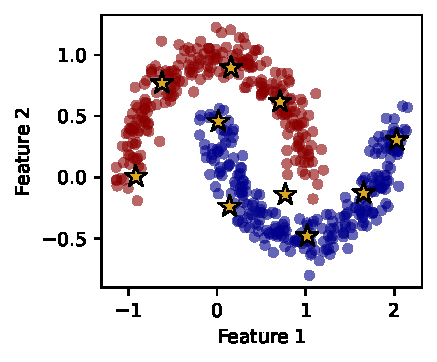
\includegraphics[height=6cm]{images/ssl/moon.pdf} % first figure
    \end{minipage}\hfill
    \begin{minipage}{0.44\textwidth}
        \centering
        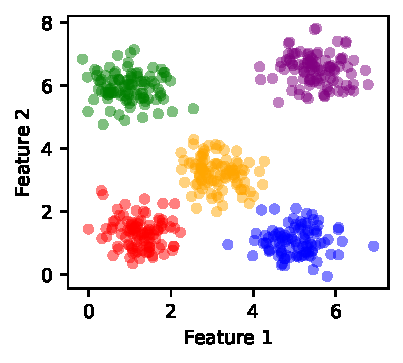
\includegraphics[height=6cm]{images/ssl/clusters.pdf} % second figure
    \end{minipage}
    \caption{Smoothness and cluster assumptions. \textbf{Left}: The moon dataset representing smoothness between 
        data points of each class. \textbf{Right}: The cluster assumption 
        illustrated with a toy example.}
    \label{fig:moon_cluster}
    \end{figure}

\begin{figure}[h]
    \centering
    \begin{minipage}{0.4\textwidth}
        \centering
        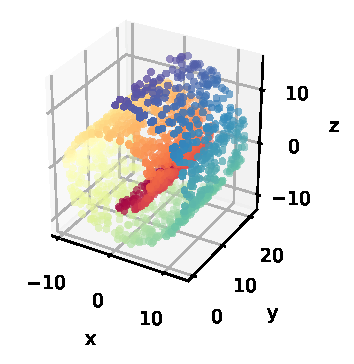
\includegraphics[height=6cm]{images/ssl/swiss_roll_3d.pdf} % first figure
    \end{minipage}\hfill
    \begin{minipage}{0.55\textwidth}
        \centering
        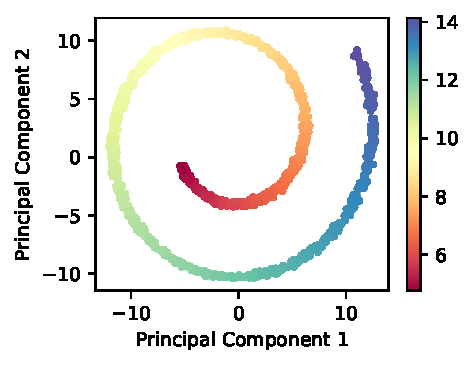
\includegraphics[height=6cm]{images/ssl/swiss_roll_pca.pdf} % second figure
    \end{minipage}
    \caption{Illustration of the manifold assumption. 
        \textbf{Left}: Data points are distributed in a high-dimensional space. 
        \textbf{Right}: The data points lie on a lower-dimensional manifold.}
    \label{fig:swiss_roll}
\end{figure}

\subsection{The Manifold Assumption}
\textbf{Assumption}: The data lies on a low-dimensional manifold embedded in a 
high-dimensional space.

This assumption is based on the idea that the data is not distributed uniformly 
in the input space, but it is concentrated on a lower-dimensional manifold.
It is fundamental to avoid problems related to the curse of dimensionality, 
which can lead to overfitting and poor generalization because of sparse data.

In Figure \ref{fig:swiss_roll}, the manifold assumption is illustrated with the 
Swiss roll dataset. The data points are distributed in a three-dimensional 
space, but they lie on a two-dimensional manifold. In general, the principal 
components analysis (PCA) can be used to reduce the dimensionality of the data, 
and in this specific case principal components are respectivlely the $x$ and $z$ 
axes.


\subsection{The Labeling Algorithm}
Classical pseudo-labeling methods usually train the teacher model on the labeled 
data and then they keep it fixed to predict the labels on the unlabeled data. 
The pseudo-labels are then used to train the student model, which is a copy of 
the teacher model. The student model is finally trained on the pseudo-labelled 
data.

On the other hand, on Meta Pseudo-Labels \cite{pham2021meta}, the teacher is 
trained along with the student model. In particular the student model is trained 
on the pseudo labels generated by the teacher model, and the teacher is trained 
on the performance of the student model on the labeled data. This process is 
repeated until the student model converges reaching a better performance 
with respect to the teacher. Therefore, the teacher model is updated to 
maximize the performance of the student.

In a more formal way, Pseudo Labels aims to optimize the student's 
loss function $CE(T(x_u, \theta_T), S(x_u, \theta_S))$, with the pseudo-labels 
generated from the teacher on the unlabeled data:

\begin{align}
    \theta_S^{PL} &= \arg \min_{\theta_S} \mathbb{E}_{x_u}\left[
        {CE(T(x_u, \theta_T), S(x_u, \theta_S))}\right] 
        \label{eq:pl_student_param}\\
        &:=
        \arg \min_{\theta_S} \mathcal{L}_u(\theta_T, \theta_S) \nonumber
\end{align}

where $T(x_u, \theta_T)$ is the pseudo target generated by the trained teacher 
model with its parameters $\theta_T$ already optimized and fixed. 
Therefore, the final goal of 
Pseudo Labels is to have a lower student loss with respect to the teacher on 
the labelled data:

\begin{align}
    \mathbb{E}_{x_l, y_l}\left[CE(y_l, S(x_l, \theta_S^{PL}))\right]
    &\leq
    \mathbb{E}_{x_l, y_l}\left[CE(y_l, T(x_l, \theta_T))\right]
    \qquad \Longleftrightarrow 
    \label{eq:pl_student_loss}\\
    \mathcal{L}_l(\theta_S^{PL})
    &\leq\
    \mathcal{L}_l(\theta_T) 
    \nonumber
\end{align}

Combining Equations (\ref{eq:pl_student_param}) and (\ref{eq:pl_student_loss}) 
it is possible to notice that the student loss $\mathcal{L}_l(\theta_S^{PL})$ 
depends on the teacher parameters $\theta_T$. Therefore, it could be possible 
get a better optimization of the teacher model to reduce the student loss. 
This is the main idea behind Meta Pseudo-Labels.
The final student loss $\mathcal{L}_l^*(\theta_S^{PL})$ will be the following:

\begin{align}
    \mathcal{L}^*_l(\theta_S^{PL*}) &= \min_{\theta_T} \mathcal{L}_l(\theta_S^{PL}(\theta_T))
    \label{eq:pl_student_loss_final} \\
    \text{where} \qquad \theta_S^{PL}(\theta_T) &= \arg\min_{\theta_S} \mathcal{L}_u(\theta_T, \theta_S)
\end{align}

However, the dependency of
%
\chapter{Methods}
\label{chpt:methods}

\section{Traditional Computer Vision-based Approach}
\label{sec:methods_traditional_cv}

This section is related to all the experiments done on the traditional computer 
vision-based approach. The general scheme of the driver's attention model is 
shown in Figure \ref{fig:driver_attention}. 
The model is divided into four main stages: data synchronization, homography 
projection of the gaze, scene perception, and the driver's behavioral model. 

The data synchronization stage is responsible for aligning the data from the 
different sensors. In particular it is important that gaze data and 
images from the 
eye-tracking glasses are well synchronized each other and with video frames 
from the camera installed on the roof top of the car.

The homography projection of the gaze stage is responsible for projecting the 
gaze of the driver from the ETG camera plane to the roof top camera plane.
In this way we have a wider, more stable and accurate representation of 
the outside environment.
It is possible to 
estimate the homography transformation making the approximation that the matched 
keypoints are far away enough from the vehicle. This is a reasonable 
approximation since the driver is usually looking at the road and the objects 
far away from the vehicle. Moreover, the baseline of the stereo vision system is 
small compared to the depth of the keypoints.
The optimal way to estimate the projection would be through the epipolar 
geometry, estimating the fundamental matrix and the essential matrix. 
However, we have an uncalibrated stereo setup, and the baseline between the two 
cameras is not fixed. Even though it could be possible to integrate GPS data 
to estimate the two matrices, there is a consistent noise error that affects 
accuracy of the estimation.
The homography estimation is then divided in three steps: detection of keypoints 
in the two images through the SIFT algorithm, matching of the keypoints through 
RANSAC, and estimation of the homography matrix through the least squares method.

The scene perception stage is responsible for detecting and tracking the vulnerable 
users in the scene, such as pedestrians and cyclists. The detection is done 
through the YOLOv8 algorithm and the tracking through ByteTrack. In this way 
it is possible to compare the gaze of the driver with the state of the targets, 
including their position.

Finally, on the top, there is the driver's attention model. The responsibility 
of this block is to classify dangerous scenarios given the data from the 
driver and the scene. However, this block is sensitive to the quality of the 
signals of the previous stages.

\begin{figure}
    \centering
    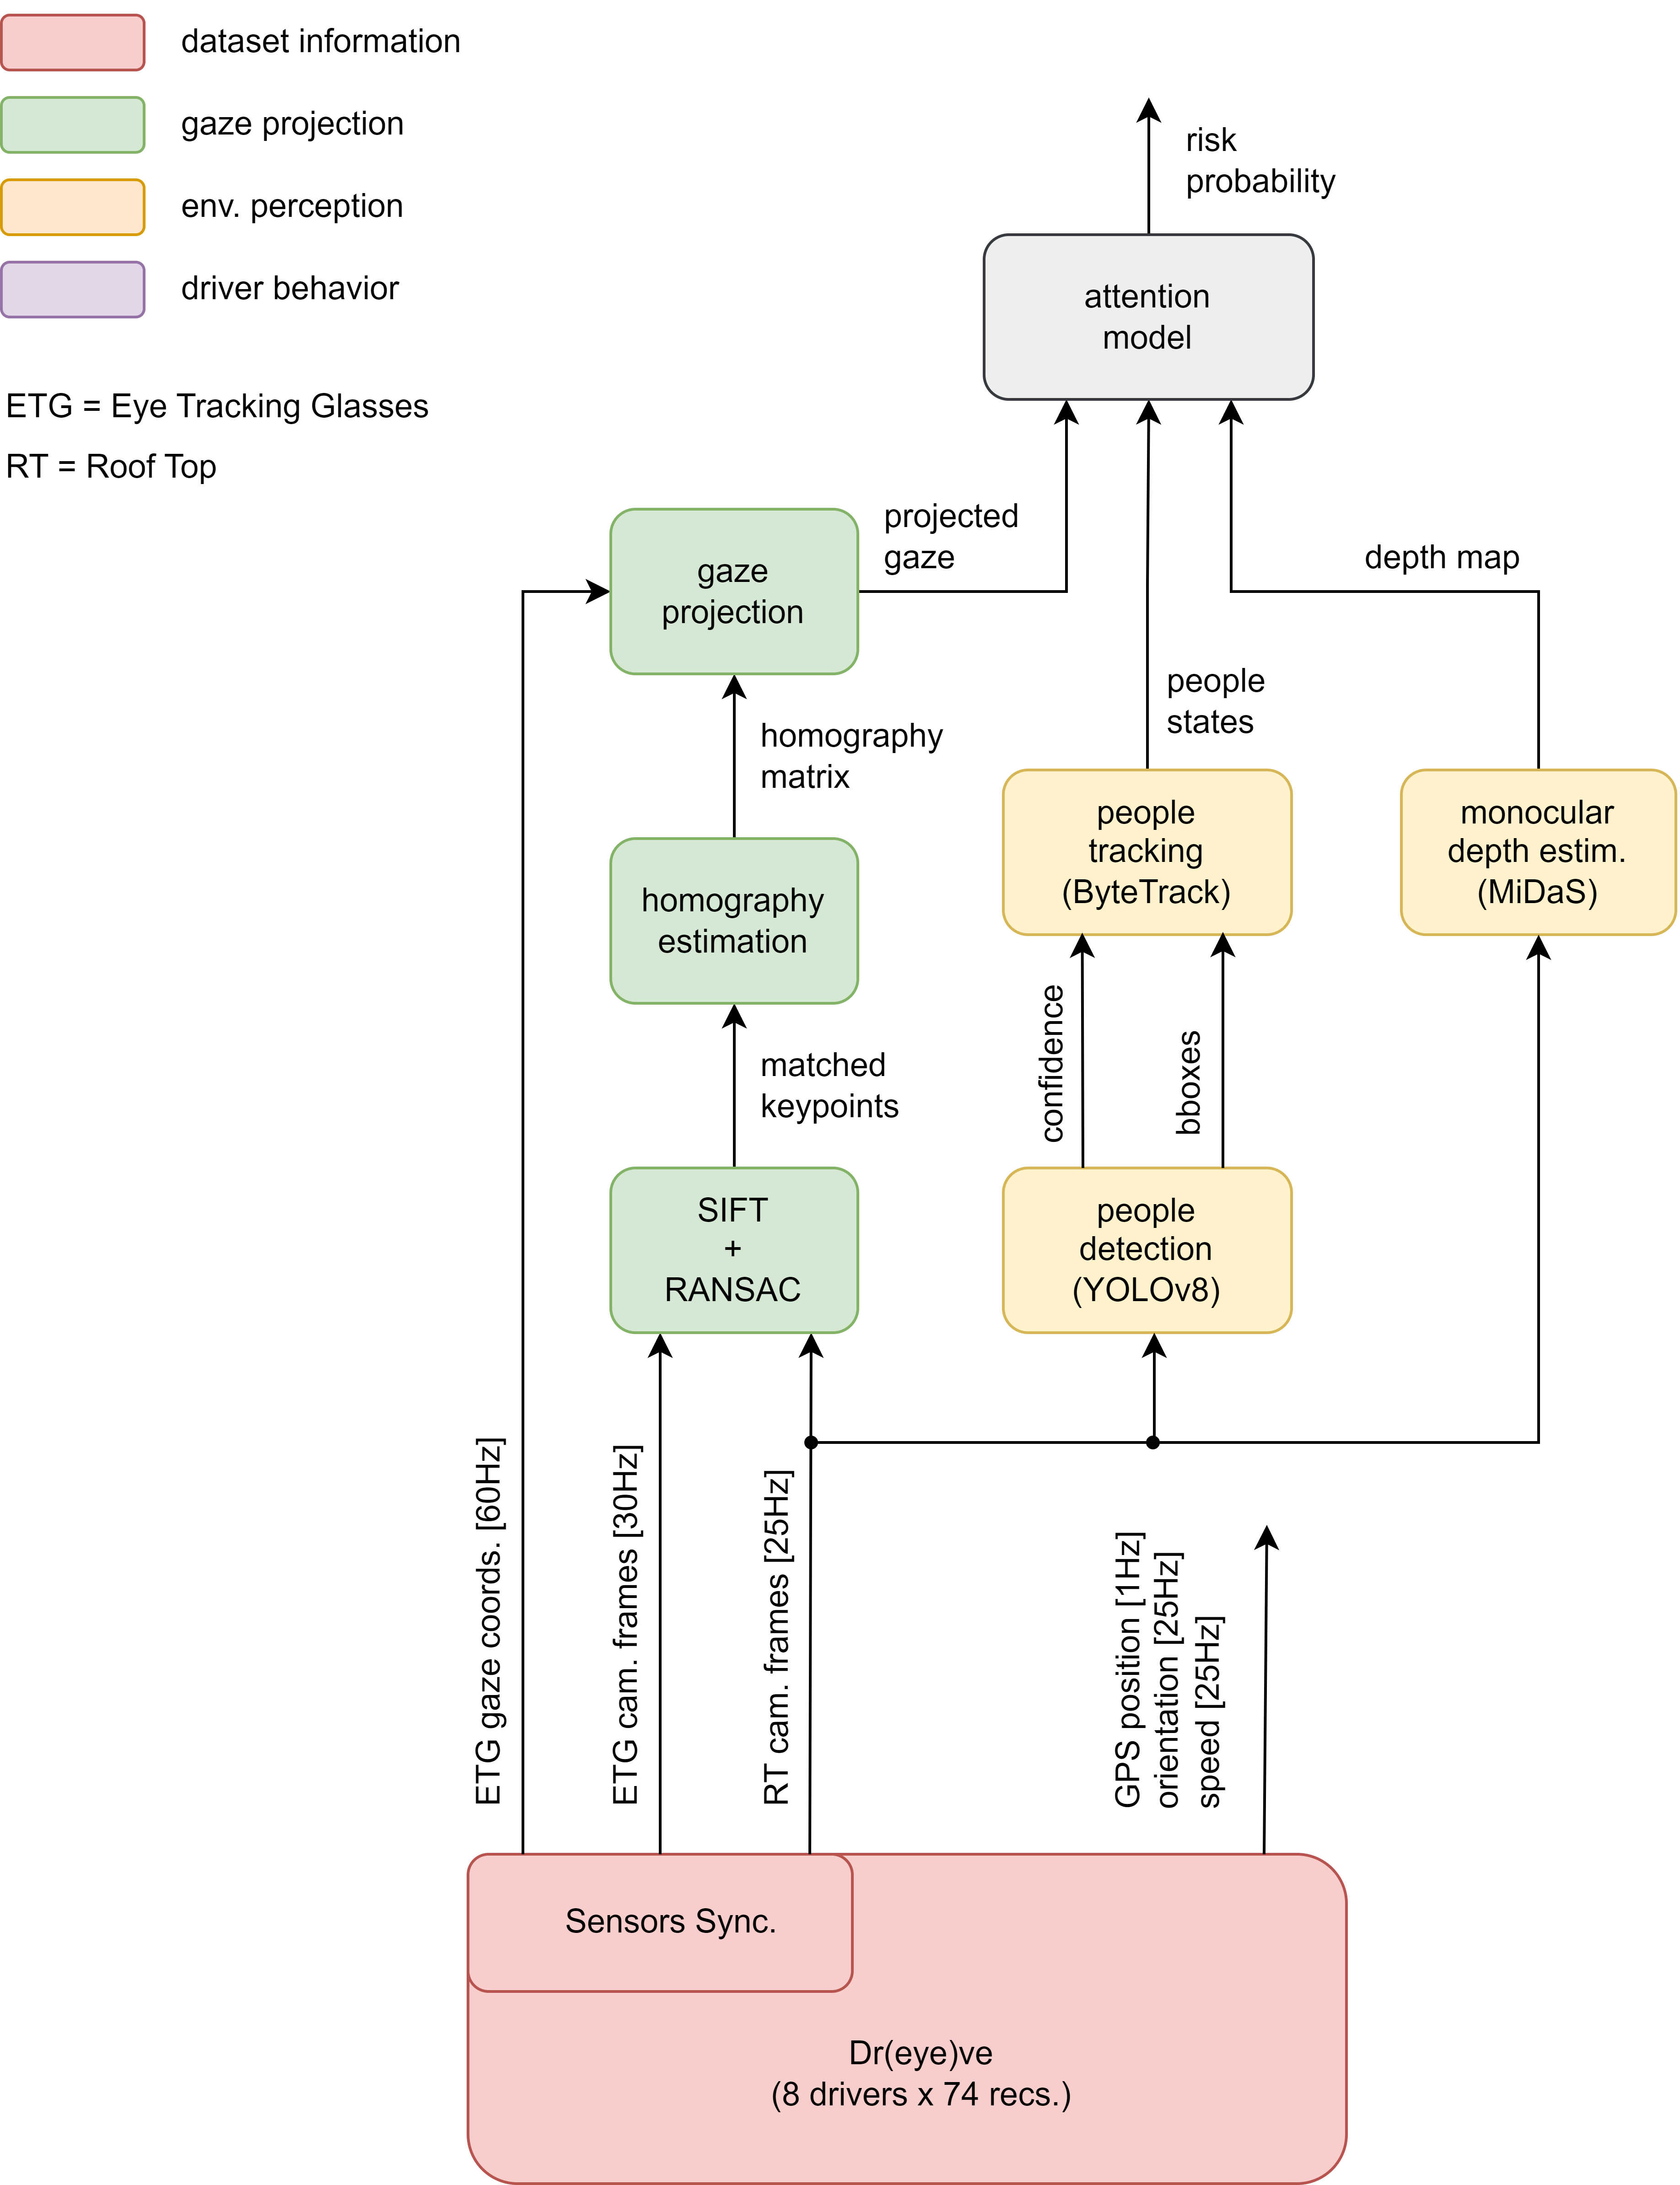
\includegraphics[width=0.9\textwidth]{images/dreyeve/classic_scheme.png}
    \vspace*{0.6cm}
    \caption[Traditional computer vision-based driver's attention model]
    {The overall driver's attention scheme. It is divided into four main 
    stages: data synchronization, homography projection of the gaze, scene 
    perception and the driver's behavioral model.
    }
    \label{fig:driver_attention}
\end{figure}

\subsection{Homography Data Structure}
The Dr(eye)ve dataset is composed of 74 sequences of five minutes each. 
Moreover, the two cameras are not synchronized. 
The ETG camera has a frame rate of 30 fps, while the roof top camera has a 
frame rate of 25 fps. It is also important to notice that there are some videos 
that was recorded at slightly different frame rates. All the synchronization data 
are provided in the dataset.

Therefore, we decided to implement 
an interface to preprocess all the frames and synchronize them.
After the synchronization, we compute all the homographies and store them in a 
file. This file is then used to project the gaze of the driver in the roof top 
camera plane.
Furthermore, we chose to store other informations related to the quality of the 
estimation.
The data structure is described in Figure \ref{fig:homography_data_structure}:
it is a list of lists where each element is a unique sample that has the 
following fields: the gaze coordinates in the ETG and RT camera planes, the 
homography matrix, detected keypoints on the two planes, and the number of 
matchings between them.

\begin{figure}
    \centering
    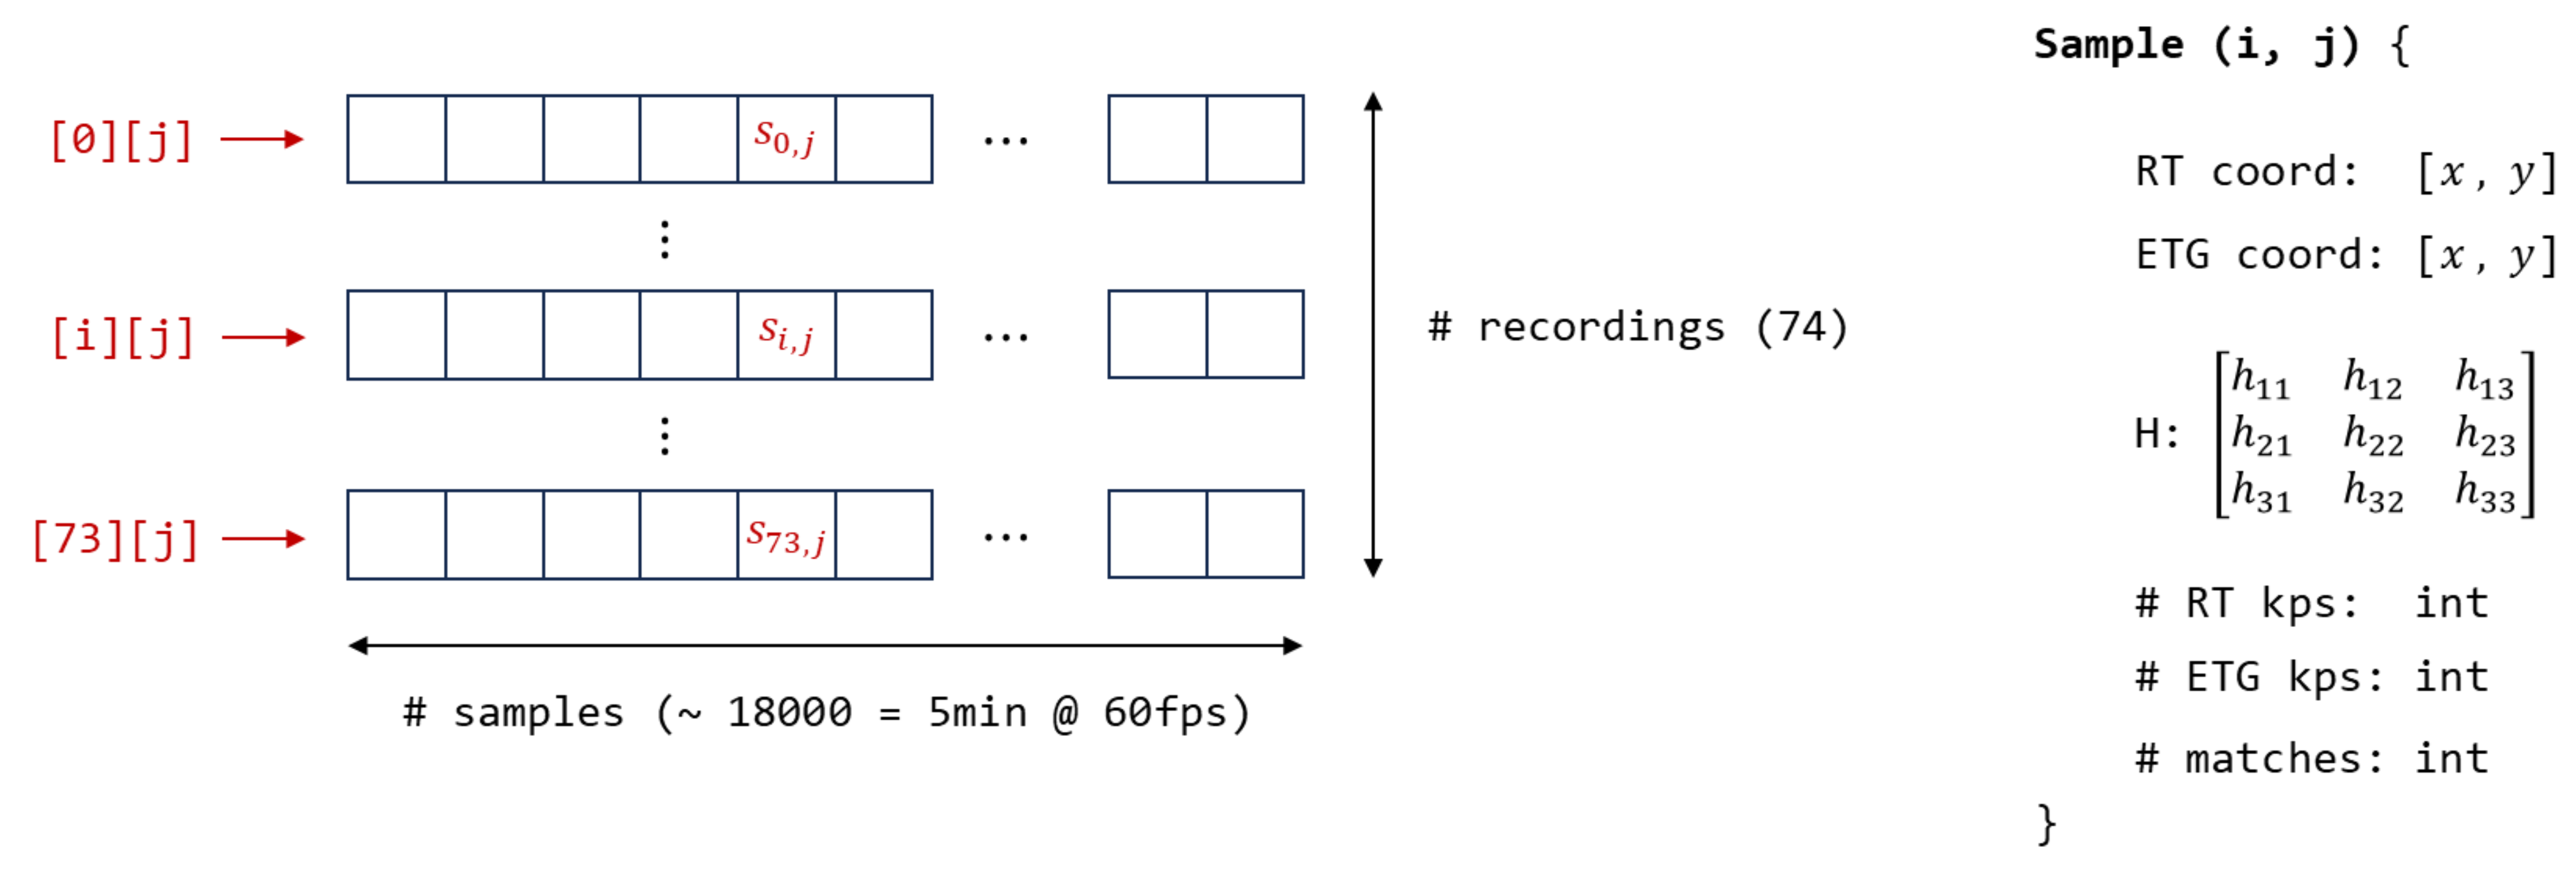
\includegraphics[width=\textwidth]{images/dreyeve/homography_data.png}
    \caption[Data structure to store homographies]
    {The data structure used to store the homographies.
    \textbf{Left}: Each element is a specific sample in the i-th video, at 
    the j-th frame.
    \textbf{Right}: The attributes of each sample.}
    \label{fig:homography_data_structure}
\end{figure}

\subsection{Stereo Camera System Setup}
The cameras recording system can be reconducted to an uncalibrated stereo vision 
setup. In particular, the two cameras are not aligned and the baseline is not 
fixed. However, this is a problem for the projection of 3D world points between 
the two cameras. In fact, homography is a planar transformation, 
and it is possible to estimate the projection matrix if keypoints lie on the 
same plane.
For this reason we decided to make the approximation that the 
keypoints are far away enough from the vehicle. This is a reasonable 
approximation since the driver is usually looking at the road and the objects 
far away from the vehicle. Moreover, the baseline of the stereo vision system is 
small compared to the average depth of the keypoints.

In this way, it is not necessary to know intrinsic and extrinsic parameters of 
the cameras, such as focal length, resolution, and distortion coefficients. 
This approach is also proposed in the Dr(eye)ve paper \cite{dreyeve}.


\subsection{Targets Data Structure}
From the Dr(eye)ve dataset, we extracted the bounding boxes of the vulnerable 
road users, such as pedestrians and cyclists.
Moreover, through ByteTrack \cite{bytetrack}, we tracked the targets to have a 
spatio-temporal representation of the scene. Then, we compare the projected gaze 
of the driver with the location of targets. 

However, it is necessary to consider the quality of the tracking. Even though 
ByteTrack was specifically designed to track also overlapping objects, in driving 
scenarios it is not uncommon to have tracking failures. To partially mitigate 
the problem, we set two different states for each target: a 
\emph{detection} state and an \emph{observation} state.
\begin{itemize}
    \addtolength\itemsep{-2mm}
    \item \textbf{Detection}: the target is being detected and tracked by the algorithms.
    \item \textbf{Observation}: the target is being observed by the driver.
\end{itemize}

\begin{figure}
\centering
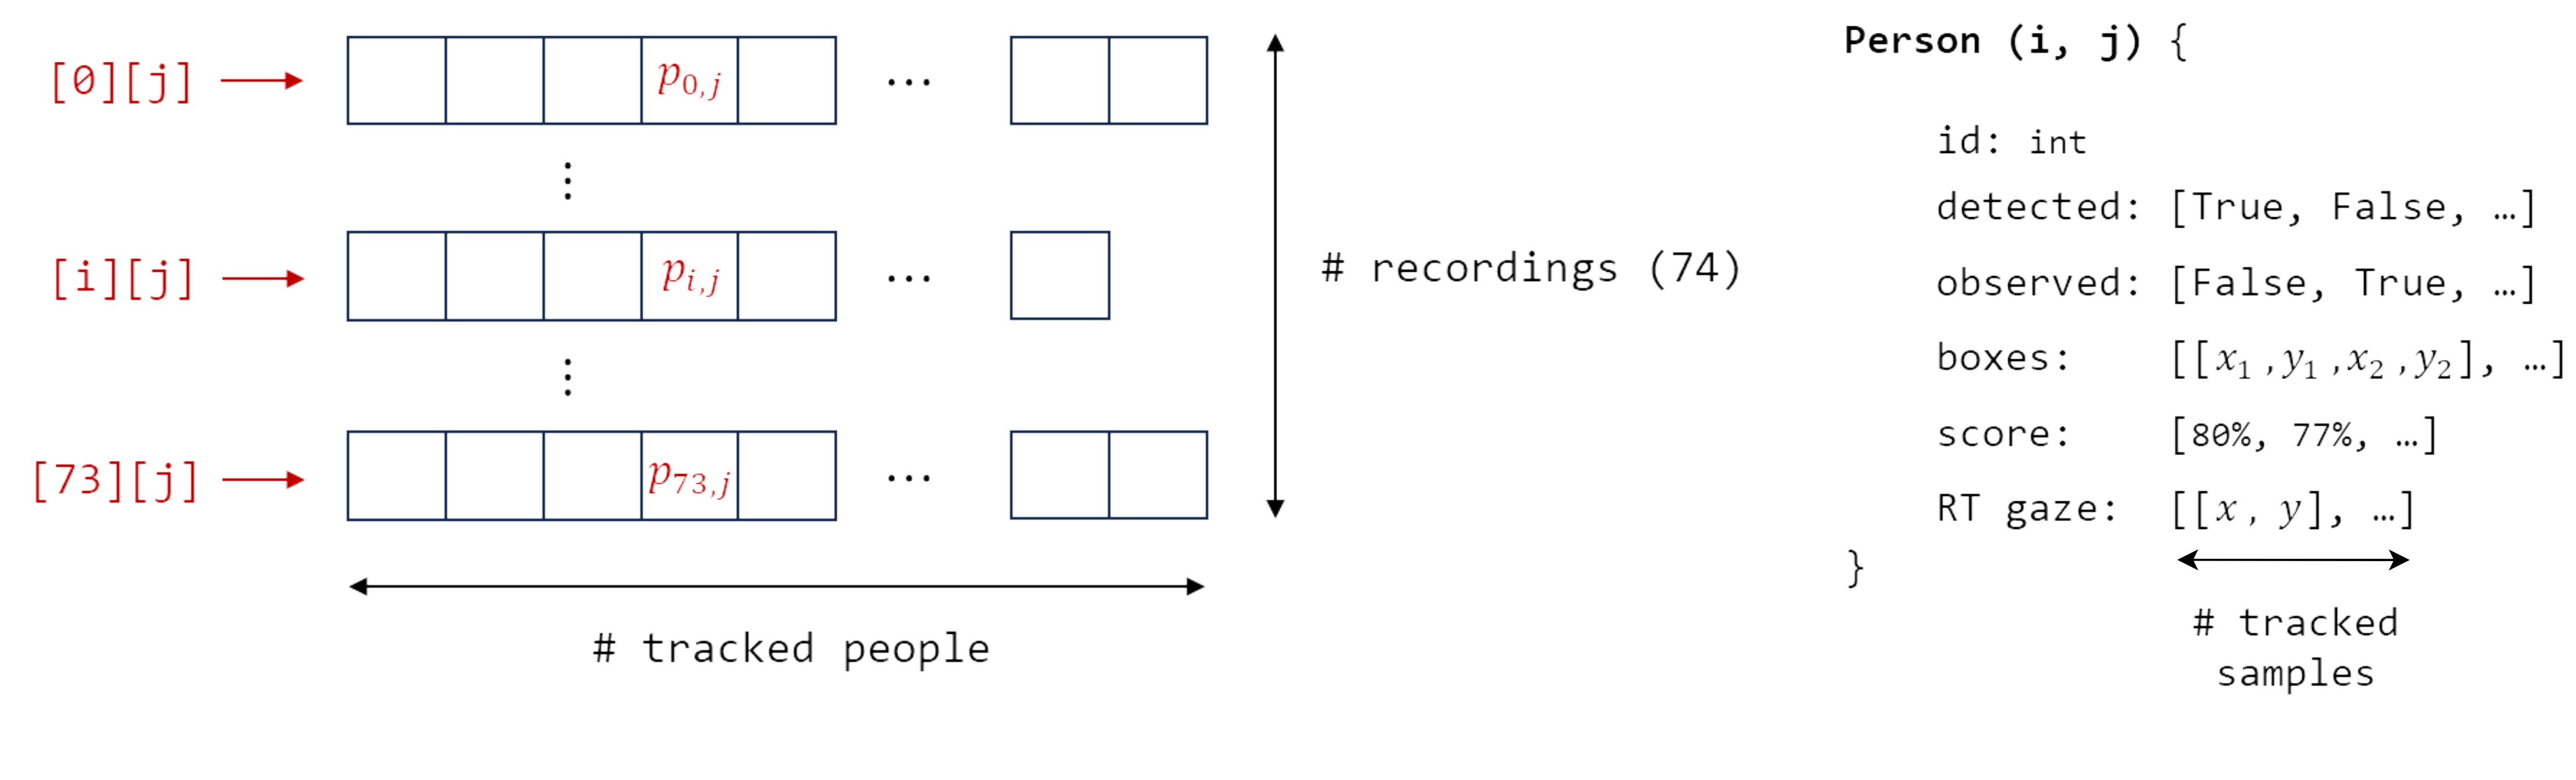
\includegraphics[width=\textwidth]{images/dreyeve/targets_data.png}
\caption[Data structure to store targets' states]
{The data structure used to store targets' states.
\textbf{Left}: Each element is a specific person, which contains the set of 
states during all its tracking.
\textbf{Right}: The attributes of the tracked person during time.
}
\label{fig:targets_data_structure}
\end{figure}
Through this approach, we can make sure if a person is both detected by the 
algorithm and observed by the driver. Without storing the detection data, there 
can be some unclear situations where the driver is looking at a target that is 
partially or completely occluded. That can happen because ByteTrack keeps the 
tracking of occluded targets through a Kalman filter. 
The data structure is represented in details 
in Figure \ref{fig:targets_data_structure}: it is a list of lists where each 
element is a unique person that has been tracked in the respective video.

Each person has the following list of states: a unique tracking ID, the 
detection states, the observation states, the bounding boxes' coordinates with 
the confidence score, and the coordinates of the projected driver's gaze.

\subsection{Adding Depth Information}
Targets' depth information can be very informative for the driver's attention 
model. In fact, the driver is usually more interested in the objects that are 
closer to the vehicle.
Considering the cameras' setup there are three main ways to include depth 
information of the scene: using a neural network to estimate the depth of the 
detected objects from the bounding box dimensions, leveraging the stereo vision 
data and car's location information (GPS and speed) to estimate the depth of 
similar keypoints in consecutive timeframes, or to compute a monocular depth 
map through a pretrained model.

The first approach is the simplest and the fastest, but it is also the less 
accurate. In fact the depth of an object is not only related to its dimensions, 
especially for people. Bounding boxes can vary depending on the target age, pose, 
occlusions and if they are riding a vehicle, like a bicycle. 
Moreover, a custom calibration should be made at least for each camera model, 
with its dedicated lens and image sensor. Image distortion could heavily affect 
the quality of predictions. However, this is not feasible in our case because 
we do not have any ground truth information to fine-tune the model.
Some recent works on targets' depth estimation with stereo vision systems were 
proposed in \cite{li2019stereo}, \cite{Peng_2020_CVPR}. There are also studies 
on retrieving the depth of objects from monocular images \cite{bbox_mde}.

The second approach is the most accurate and robust, but it requires an accurate 
calibration of the stereo vision system to perform well. Moreover, data depth 
is only related to correspondent keypoints. This means that if no matching 
keypoints related to a target are found, it is not possible to estimate its 
depth. Finally, the stereo vision system is not always reliable, especially when 
it is uncalibrated and the baseline is not fixed and relatively small compared to 
the average depth of the keypoints. 
Recently some self-calibration methods have been proposed 
\cite{sfm_self_calibration1}, \cite{sfm_self_calibration2}.
The roof top camera has a wide field of 
view because it uses a wide angle lens, and then an anti-distortion algorithm 
is computed. This affects the quality of the depth estimation.

The third approach is the most versatile and suitable to the specific application.
In fact, the dense depth map computed by the pretrained model is not related to the 
ETG camera and allows to estimate the depth of all the objects in the scene.
The model is trained on a large dataset and is able to generalize well to 
different scenarios. The only drawback is that the depth map is not absolute. 
This means that it is not possible to estimate the distance of objects in meters, 
but through a relative scale depending on the maximum and minimum depths of the 
scene. However, this should not be able to compromise the quality of the 
driver's attention model because that is the same approach we use as humans 
when driving. However, we actually compute a hybrid approach where we use a sort 
of stereo vision system through our eyes and our knowledge and past experience 
to make an approximate estimation of the depth of the objects.
In the experiments section we will show the performance of pretrained MiDaS 
\cite{midas}.

\begin{figure}
\centering
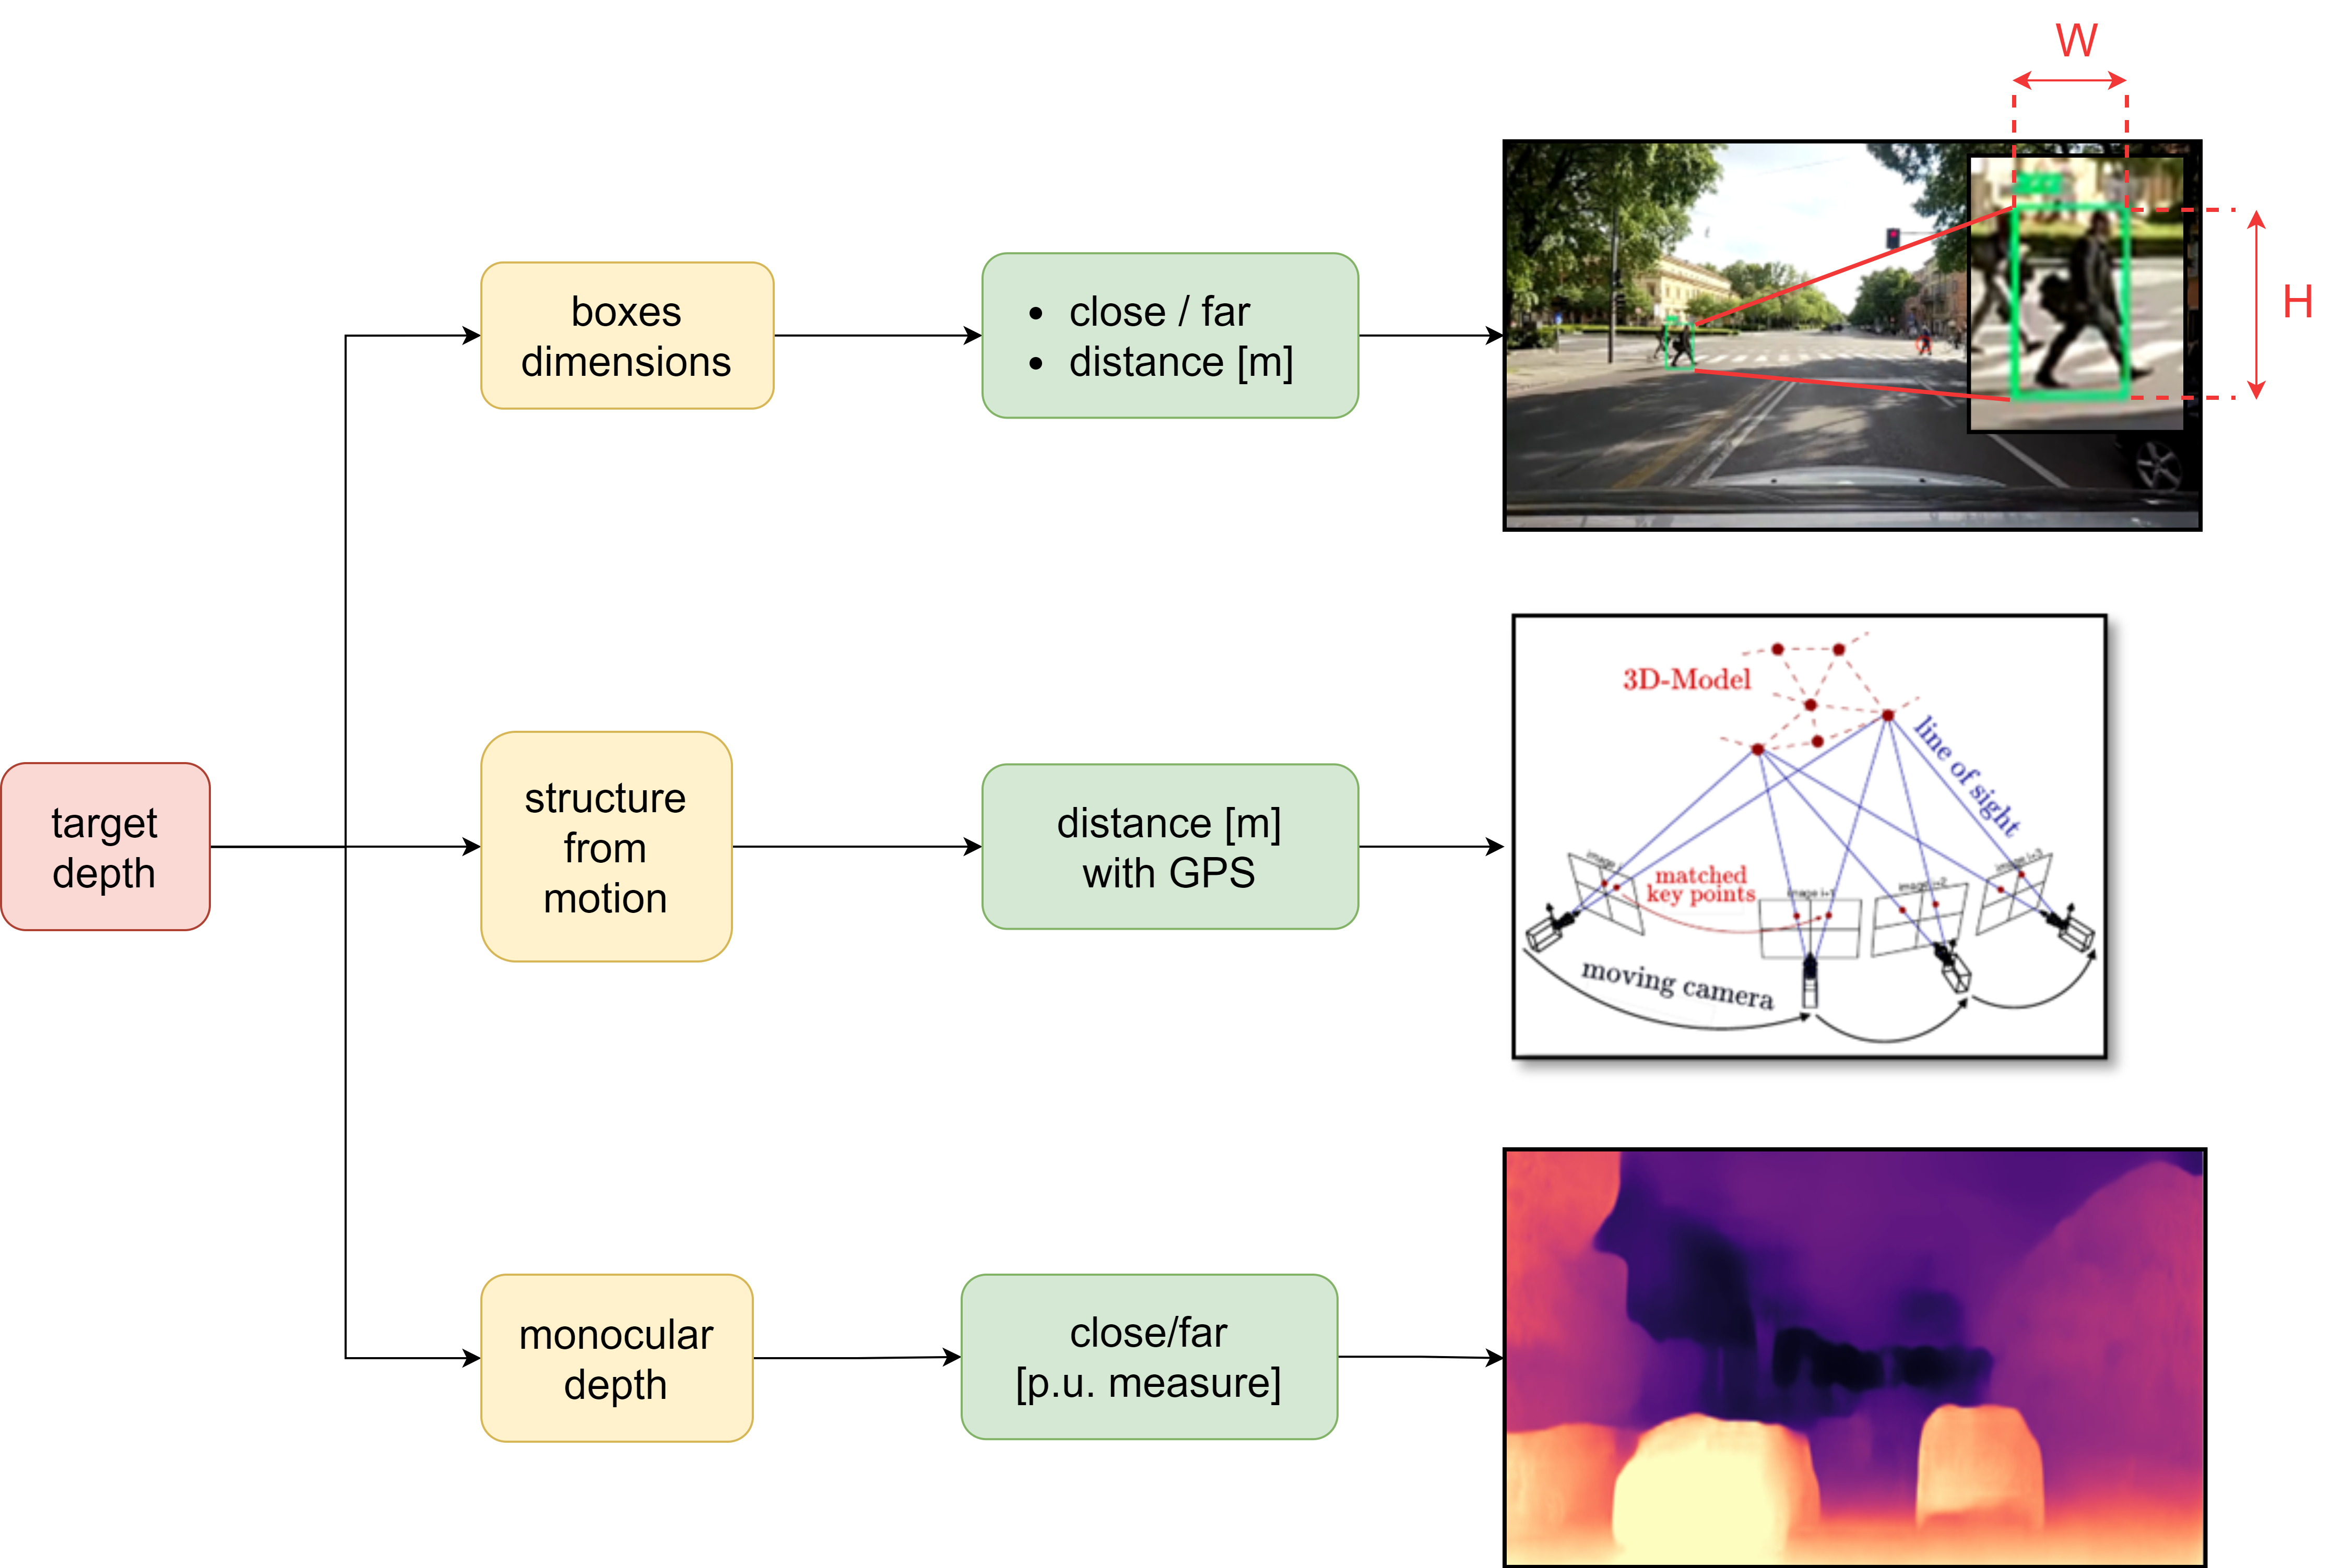
\includegraphics[width=\textwidth]{images/dreyeve/depth_estimation.png}
\caption[Three possible methods to estimate targets' depth]
{Summary of the possible three methods to estimate the depth of targets.}
\label{fig:depth_estimation}
\end{figure}



\subsection{Adding Spatial Information}
Spatial information can be fundamental to analyze the driver's attention 
towards targets in the scene. In fact, the driver usually pays more attention 
to some locations of the field of view, depending on the context (e.g. type of 
road, traffic, weather conditions, crowdness, etc.).
Moreover, the double camera setup allows to have a wider field of view on the 
rooftop camera. This is particularly useful to track the gaze also when the 
driver is moving the head. 

Therefore, an initial approach is to include the spatial information of the 
gaze in the driver's attention model. In particular, we divided the roof top 
camera view in a 3x7 grid, as shown in Figure \ref{fig:rt_camera_grid}. 
This division is made to have a more detailed representation of the scene, in 
fact it is possible to notice that cells from  1 to 7 are out of interest when 
the driver is looking straight ahead. These area are 
located on the top of the image, where the driver is usually not looking at, 
except for some specific situations (e.g. traffic lights, road signs, etc.). 

Cells 8, 9, 13, 14 represent out of field of view areas, where there could be 
potential threats (e.g. a pedestrian crossing the road from the left side, 
a car crossing the road). 

Cells 10, 11, 12 are the center of the field of view, 
where the driver is usually looking at. In particular, considering the city 
center shown in Figure \ref{fig:rt_camera_grid}, area 11 captures front 
vehicles. 
Cells 10, 12, show possible targets interacting 
in the near future with the ego-vehicle 
from the road sides (e.g. the ego-vehicle approaching a crosswalk with a 
pedestrian waiting to cross the road).

Cells 15, 16, 20, 21 represent the left and sie corners out of the field of view 
of the ETG camera. These areas are similar to cells 8, 9, 13, 14, but on with 
closer targets. Therefore they are more dangerous because targets on these 
locations are more challenging to spot and the driver has less time to react.

Cell 17, 18, 19 are at the bottom-center of the field of view.
These areas cover in part the dashboard of the car, and the driver is usually 
looking at them when checking the speed, the fuel, the GPS, etc. 
Depending on the context, these areas could also cover close vehicles on the 
front of the ego-vehicle (e.g. a line of vehicles at a traffic light). 
Therefore, these areas can identify a warning when the driver is not 
looking at the road and there is a potential threat.

In general, we identified different areas of interest in the field of view of 
the driver, depending on the specific context. This is an initial equal division 
that still helps characterize the scene. However, considering the wide view of 
the roof top camera, and the distortion applied to the image, there are better 
solutions to divide the scene. For example, it is possible to make a non-equal 
division, grouping together areas that are more similar to each other.
In summary, spatial information is both informative and complicated to manage 
because it is highly dependent on the context. Therefore, it could be helpful 
to let a model learn the spatial information by itself, through a deep learning 
approach. This mainly motivates the move from the traditional computer 
vision-based approach to the deep learning-based approach.
 
\begin{figure}
\centering
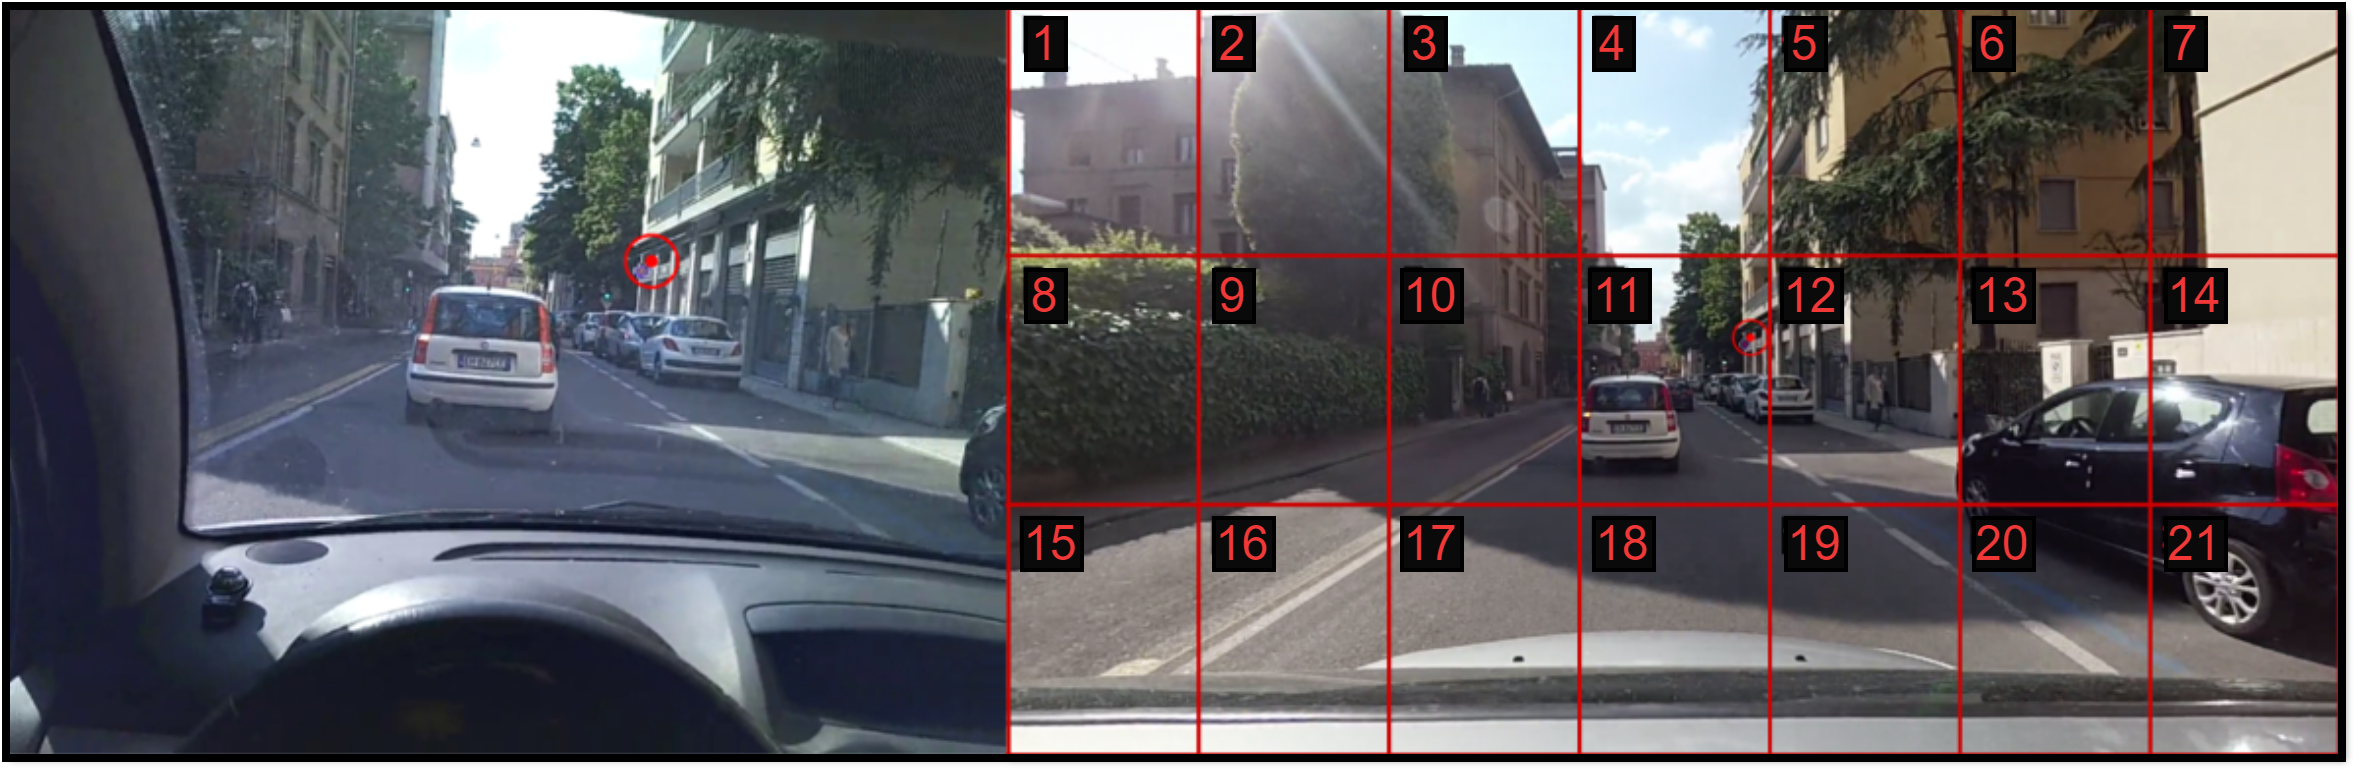
\includegraphics[width=\textwidth]{images/dreyeve/rt_cam_grid.png}
\caption[Grid division of the roof top camera view]
{Division of the roof top camera view in a 3x7 grid.}
\label{fig:rt_camera_grid}
\end{figure}


\section{Deep Learning-based Approach}
\label{sec:methods_deep_learning}
In this section we describe the deep learning-based approach to the driver's 
attention model.
Even though in the previous section we identified the main stages of the 
traditional computer vision-based approach, and many positive aspects were 
highlighted, there are also some drawbacks.
In particular, for each stage there are some simplification hypothesis that 
affect quality of inputs for the driver's attention model.

For example, the homography projection of the gaze is not perfect, and the 
approximation that the matched keypoints are far away enough from the vehicle 
is not always true. Moreover, the quality of homography estimation heavily 
depends on the quality of the keypoints' detection and matching. This can be 
compromised by the quality of the images, presence of occlusions, light and 
weather conditions, etc.

The scene perception stage is also affected by the quality of the detection 
and tracking algorithms. In particular, ByteTrack is not always able to track
overlapping objects, and the quality of the tracking is affected by the 
quality of the detection. Moreover, the detection is not always perfect, and 
there are some false positives and false negatives. 

Depth estimation stage is also affected by the quality of the pretrained 
model of MiDaS. In particular, the model is trained on a large datasets in 
completely different contexts, and it is not always able to generalize well to 
different scenarios. Moreover, the depth map is not absolute, and it is not 
possible to estimate the absoulte distance in meters.

That is why it is better to let a model learn important features automatically, through 
some classification biases used to label a dataset. We decided to use a vision 
transformer model to learn the self-attention map of the scene to detect 
potential threats.
Four main experiments were made: supervised and semi-supervised training on Dr(eye)ve, 
supervised and semi-supervised training on BDD100k.
The general scheme is shown in Figure \ref{fig:dl_approach_scheme}; as it is 
possible to notice, the scheme does not consists of some blocks to extract 
indirect features from the scene, but it is mainly focused on the deep learning 
model to learn the features by itself by camera images. In particular, the 
attention model is represented by two vision transformers: one is the teacher and 
the other is the student. The teacher is in charge of generating pseudo labels 
for the student from the unlabelled dataset. The trained student is then used 
to make the final predictions, and it is supposed to perform better than the
teacher.
\begin{figure}
\centering
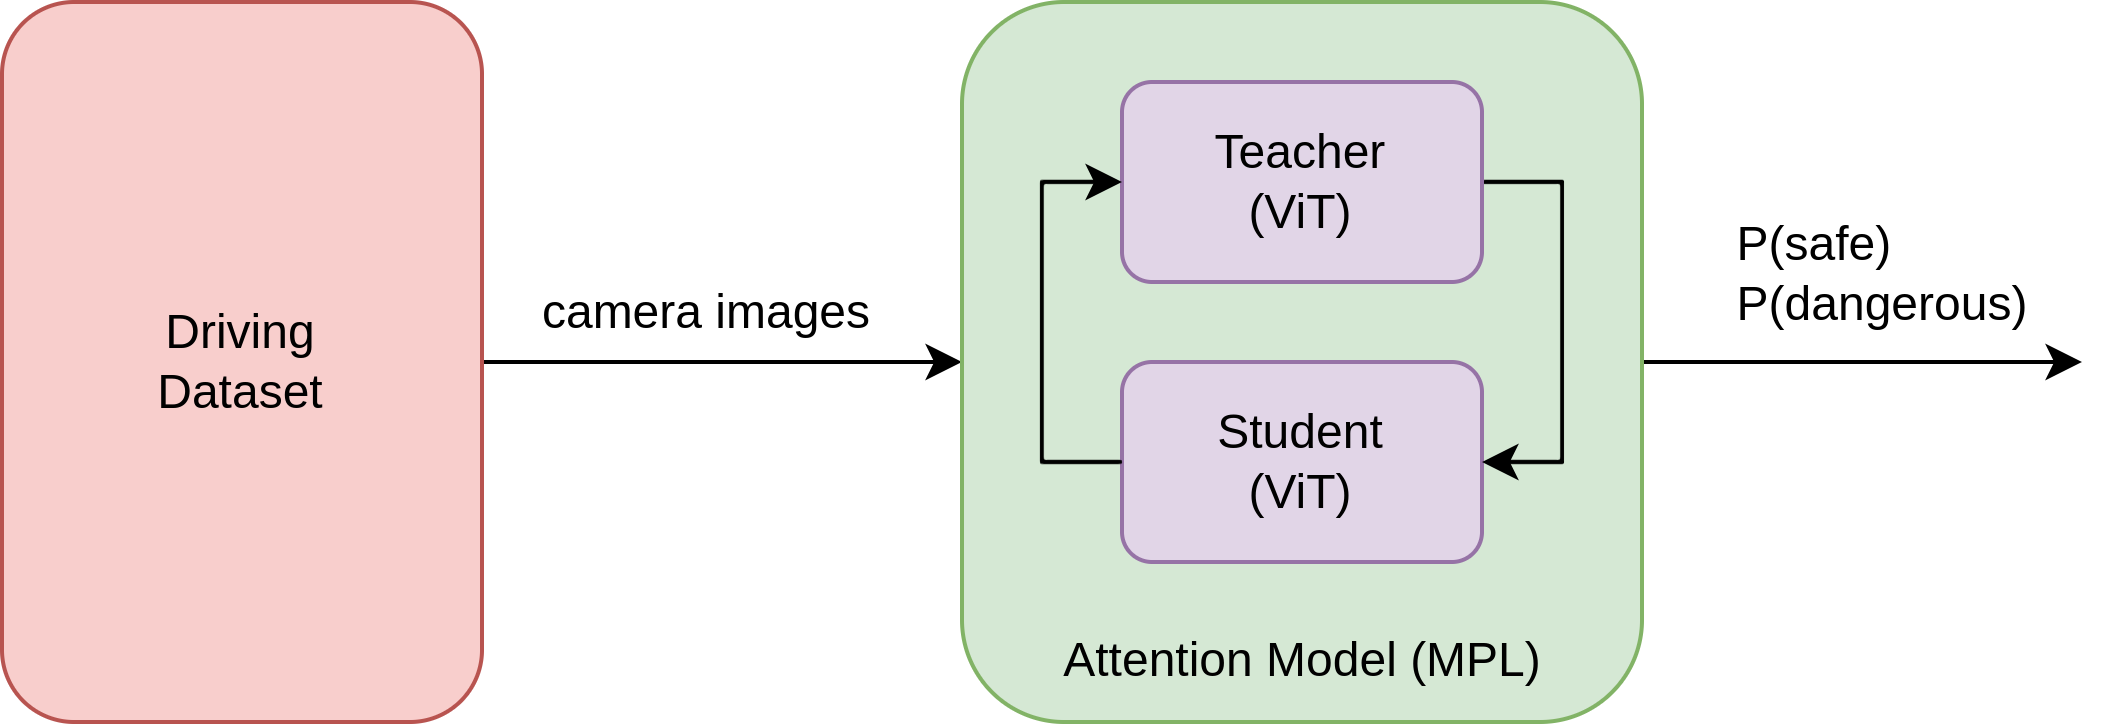
\includegraphics[width=0.85\textwidth]{images/ssl/dl_approach_scheme.png}
\vspace{0.4cm}
\caption[Deep learning-based detection model of dangerous scenarios.]
{General scheme of the deep learning-based approach for detecting
dangerous situations in driving scenarios.}
\label{fig:dl_approach_scheme}
\end{figure}

\subsection{Attention Map for Anomaly Detection}
The vision transformer model is able to learn an attention map of the scene for 
each head. This feature is useful to let the model learn many spatial relations 
between patches. The idea is to have many images labeled by humans to detect 
dangerous situations in a driving dataset. Then, we can use the attention map 
to spot critical areas of the scene that are more likely to be related to 
dangerous situations.
It is also possible to check if attention maps are consistent with the human 
decision bias with a test set.

An example of attention maps for a pre-trained multi-head vision transformer is 
shown in Figure \ref{fig:attention_maps}.
It is possible to notice that each head is focusing on some areas of the 
scene, learning different relations. This is particularly useful to detect 
anomalies in the scene, such as a pedestrian crossing the road, a car approaching 
the ego-vehicle, etc. In this particular case, the model is pre-trained on 
ImageNet, therefore many highlighted areas correspond to the presence of 
people and cars. However, in the fifht head the model extracts more general 
features to combine with the desired targets.

\subsubsection{Artificial Bias}
Labelling an entire dataset with dangerous situations is a very challenging 
task. On one hand, it is not always possible to have a clear definition of what 
is a dangerous situation. In fact, it is highly dependent on the context, the 
person who is labelling and the driving experience. On the other hand, it is 
very time consuming and expensive to label a large dataset.

Therefore, we decided to start using an \emph{artificial bias} to classify 
dangerous situations. In particular, we used two different criterias to label 
Dr(eye)ve and BDD100k datasets. In Dr(eye)ve, we used the following criteria:
a driving scene is considered dangerous if there is at least one vulnerable 
road user (e.g. pedestrian, cyclist) or one car; the scene is condidered safe 
otherwise.

In BDD100k, on the other hand, we used the following criteria: a driving scene 
is considered dangerous if there is at least one vulnerable user (e.g. pedestrian, 
cyclist) or a bicycle; the scene is considered safe otherwise.

The main motivation for the change from Dr(eye)ve to BDD100k is that the former 
dataset does not have any human annotations regarding location of targets. 
Therefore an object detector was used to accomplish the task. However, the 
quality of the detection is not always perfect, and there are some false 
positives and false negatives.
The latter, on the other hand, has high-quality human annotations for many 
classes. Moreover, it is the largest dataset available for driving scenarios, 
because each labelled frame corresponds to the frame at the tenth second of 
a driving video. This is particularly useful to leverage semi-supervised learning 
techniques, like Meta Pseudo Labels \cite{pham2021meta}.

Finally, we used two different labelling rules and two different datasets because 
Dr(eye)ve has many more frames with no other vehicles in the scene (recordings 
during night, in the countryside, etc.), while BDD100k has a high percentage of 
frames containing other vehicles. Therefore, the second labelling method is to 
have a less skewed dataset.
However, the two methods should not affect the model training, since we are 
grouping frames according to the presence of some objects, that the model should 
find out from the training set.
%
\newlength{\subfigwidth}
\setlength{\subfigwidth}{32mm}
\newlength{\horspace}
\setlength{\horspace}{.25\textwidth}
\begin{figure}
    \caption[Attention maps for a pre-trained multi-head ViT.]
    {Attention masks for a pre-trained multi-head ViT \cite{attention_vit}.}
    \centering
    \begin{tabular}{r p{\horspace} p{\horspace} p{\horspace}}
    Original & 
    \begin{subfigure}[b]{\subfigwidth}
        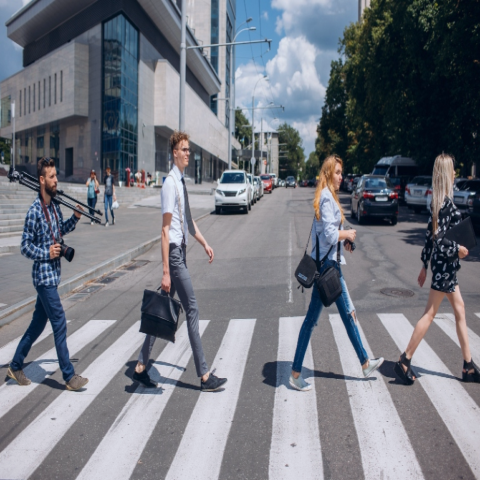
\includegraphics[width=\subfigwidth]{images/vit_attention/1/img.png}
    \end{subfigure}
    \hfill &
    \begin{subfigure}[b]{\subfigwidth}
        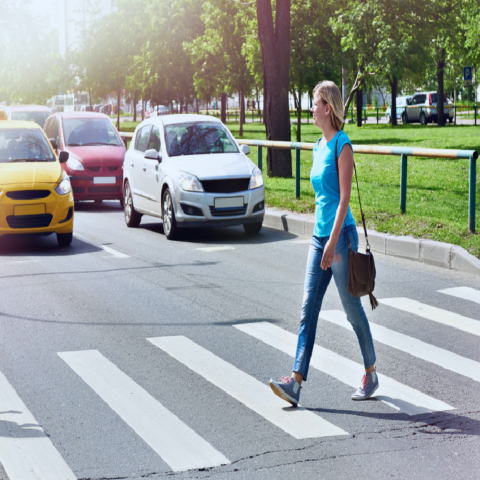
\includegraphics[width=\subfigwidth]{images/vit_attention/2/img.png}
    \end{subfigure} 
    \hfill &
    \begin{subfigure}[b]{\subfigwidth}
        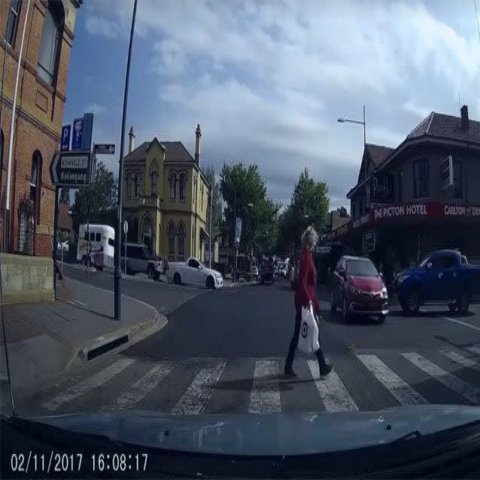
\includegraphics[width=\subfigwidth]{images/vit_attention/4/img.png}
    \end{subfigure} \\
    %
    Head 1 &
    \begin{subfigure}[b]{\subfigwidth}
        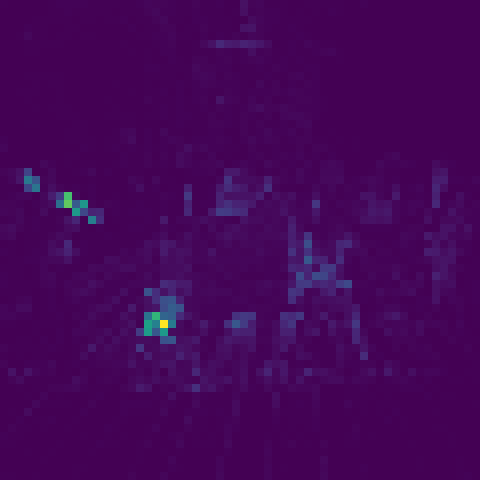
\includegraphics[width=\subfigwidth]{images/vit_attention/1/attn-head0.png}
    \end{subfigure}
    \hfill &
    \begin{subfigure}[b]{\subfigwidth}
        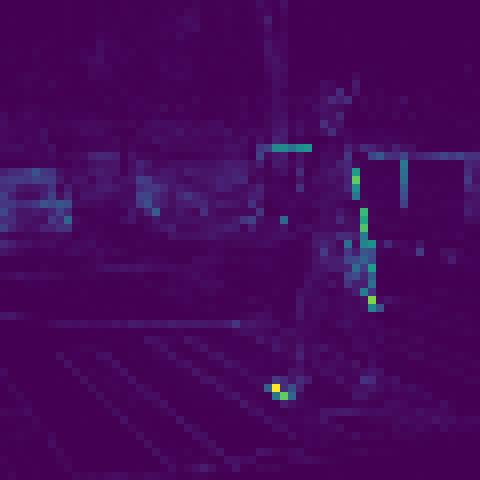
\includegraphics[width=\subfigwidth]{images/vit_attention/2/attn-head0.png}
    \end{subfigure} 
    \hfill &
    \begin{subfigure}[b]{\subfigwidth}
        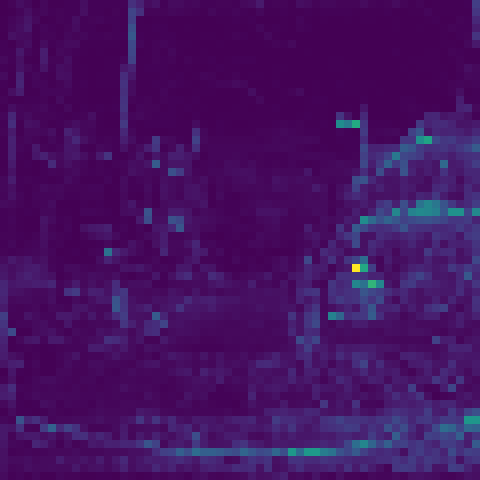
\includegraphics[width=\subfigwidth]{images/vit_attention/4/attn-head0.png}
    \end{subfigure} \\
    %
    Head 2 &
    \begin{subfigure}[b]{\subfigwidth}
        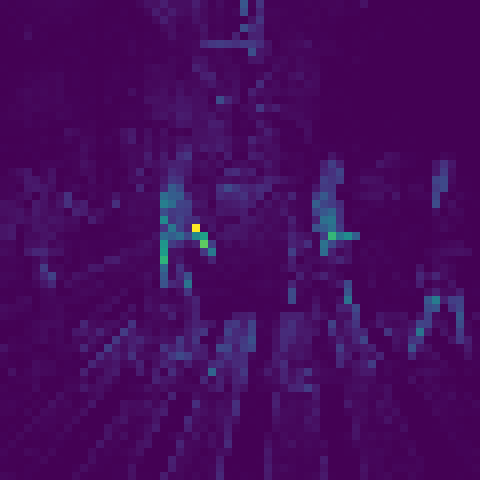
\includegraphics[width=\subfigwidth]{images/vit_attention/1/attn-head1.png}
    \end{subfigure}
    \hfill &
    \begin{subfigure}[b]{\subfigwidth}
        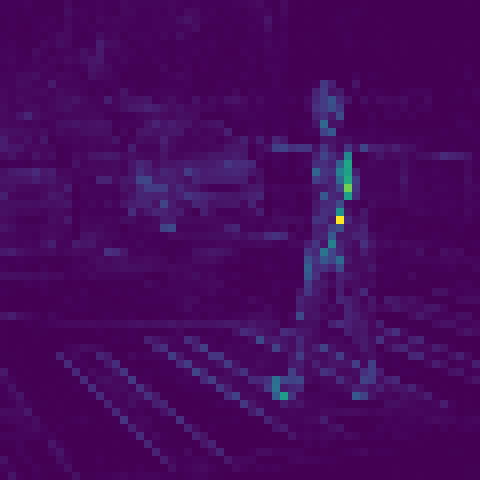
\includegraphics[width=\subfigwidth]{images/vit_attention/2/attn-head1.png}
    \end{subfigure} 
    \hfill &
    \begin{subfigure}[b]{\subfigwidth}
        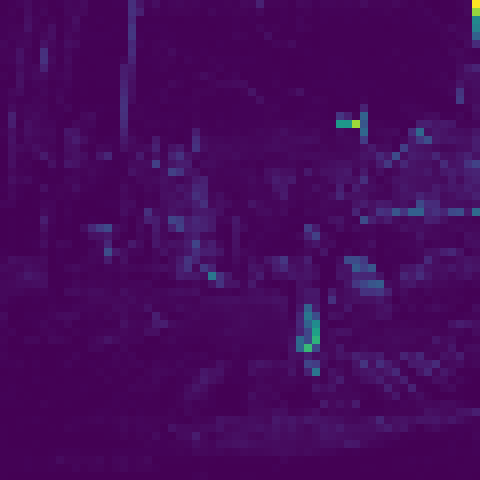
\includegraphics[width=\subfigwidth]{images/vit_attention/4/attn-head1.png}
    \end{subfigure} \\
    Head 3 &
    \begin{subfigure}[b]{\subfigwidth}
        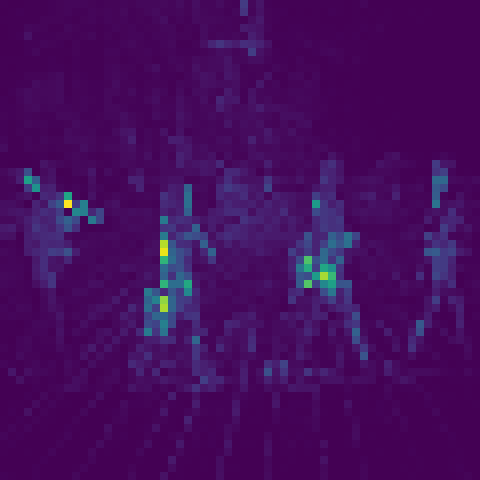
\includegraphics[width=\subfigwidth]{images/vit_attention/1/attn-head2.png}
    \end{subfigure}
    \hfill &
    \begin{subfigure}[b]{\subfigwidth}
        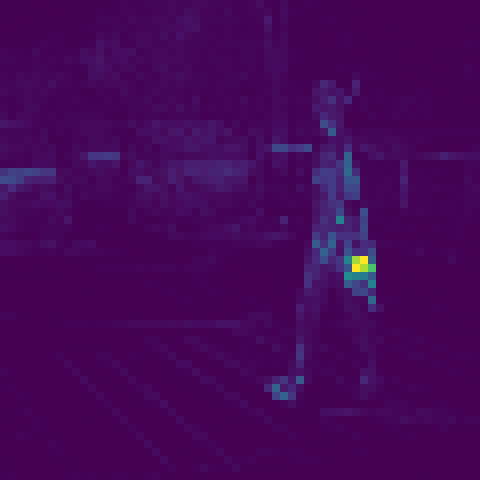
\includegraphics[width=\subfigwidth]{images/vit_attention/2/attn-head2.png}
    \end{subfigure} 
    \hfill &
    \begin{subfigure}[b]{\subfigwidth}
        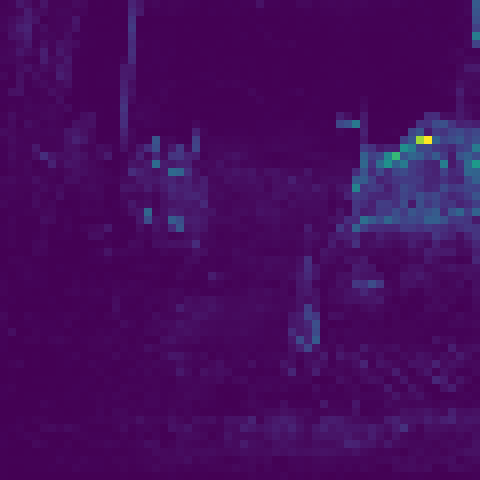
\includegraphics[width=\subfigwidth]{images/vit_attention/4/attn-head2.png}
    \end{subfigure} \\
    Head 4 &
    \begin{subfigure}[b]{\subfigwidth}
        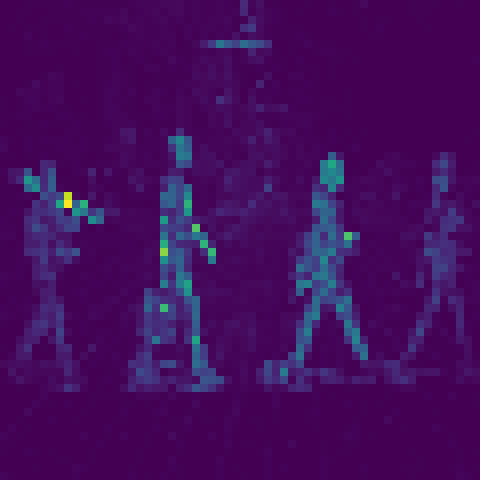
\includegraphics[width=\subfigwidth]{images/vit_attention/1/attn-head3.png}
    \end{subfigure}
    \hfill &
    \begin{subfigure}[b]{\subfigwidth}
        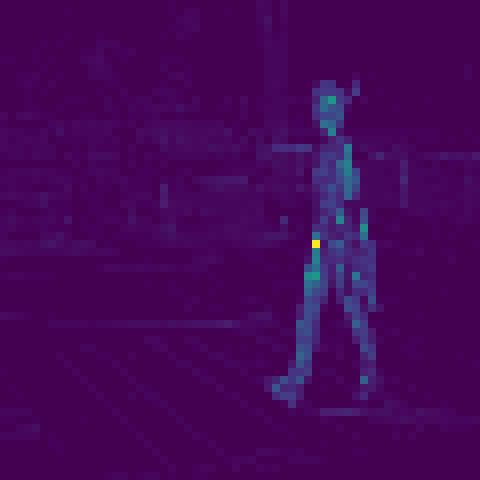
\includegraphics[width=\subfigwidth]{images/vit_attention/2/attn-head3.png}
    \end{subfigure} 
    \hfill &
    \begin{subfigure}[b]{\subfigwidth}
        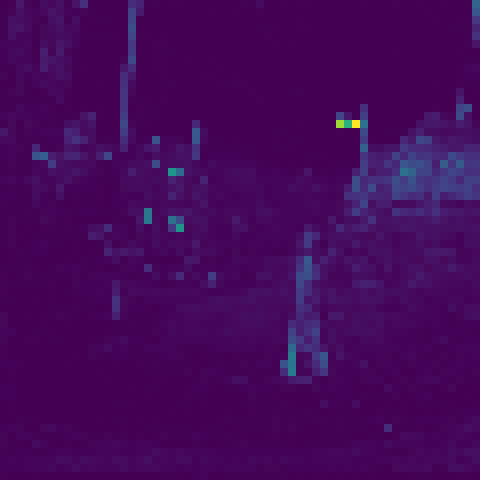
\includegraphics[width=\subfigwidth]{images/vit_attention/4/attn-head3.png}
    \end{subfigure} \\
    Head 5 &
    \begin{subfigure}[b]{\subfigwidth}
        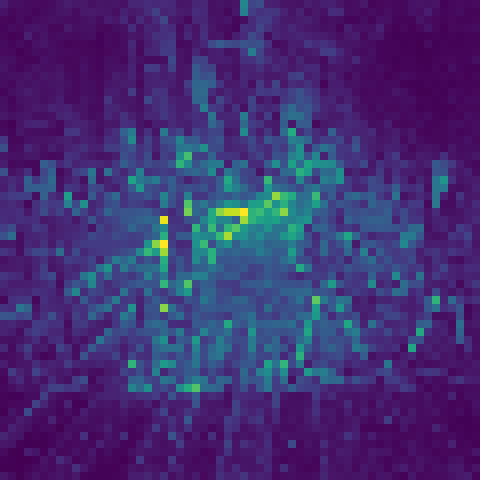
\includegraphics[width=\subfigwidth]{images/vit_attention/1/attn-head4.png}
    \end{subfigure}
    \hfill &
    \begin{subfigure}[b]{\subfigwidth}
        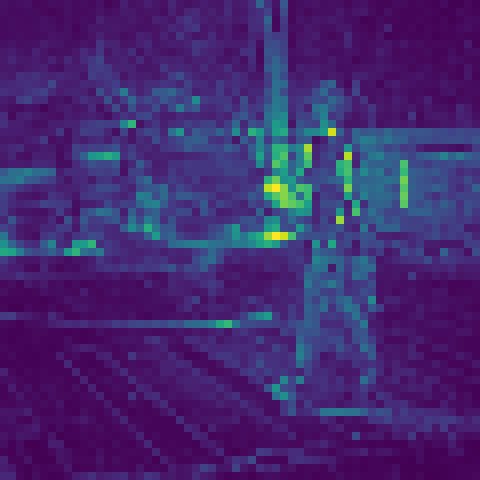
\includegraphics[width=\subfigwidth]{images/vit_attention/2/attn-head4.png}
    \end{subfigure} 
    \hfill &
    \begin{subfigure}[b]{\subfigwidth}
        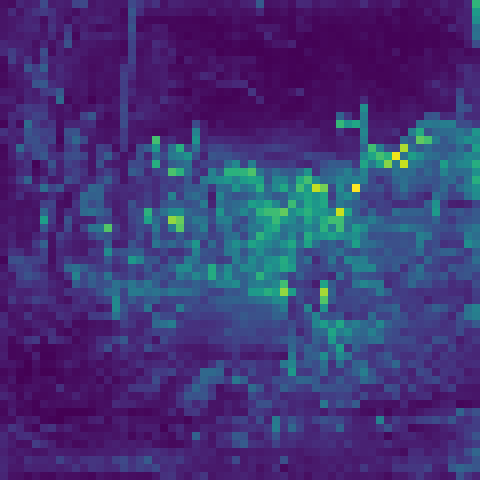
\includegraphics[width=\subfigwidth]{images/vit_attention/4/attn-head4.png}
    \end{subfigure} \\
    Head 6 &
    \begin{subfigure}[b]{\subfigwidth}
        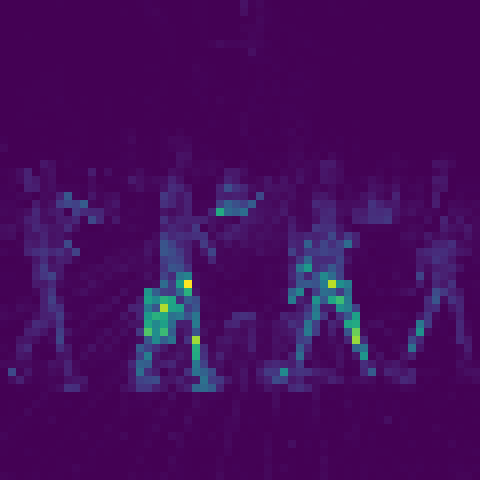
\includegraphics[width=\subfigwidth]{images/vit_attention/1/attn-head5.png}
    \end{subfigure}
    \hfill &
    \begin{subfigure}[b]{\subfigwidth}
        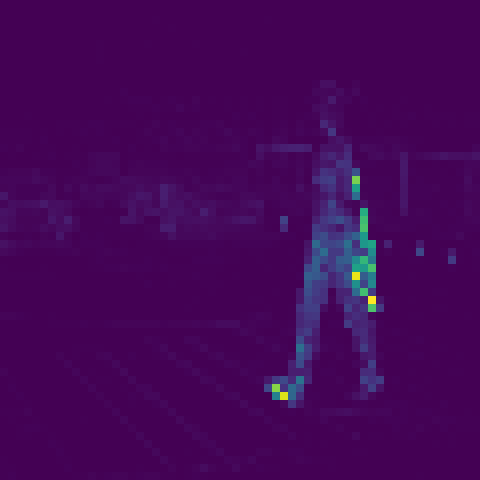
\includegraphics[width=\subfigwidth]{images/vit_attention/2/attn-head5.png}
    \end{subfigure} 
    \hfill &
    \begin{subfigure}[b]{\subfigwidth}
        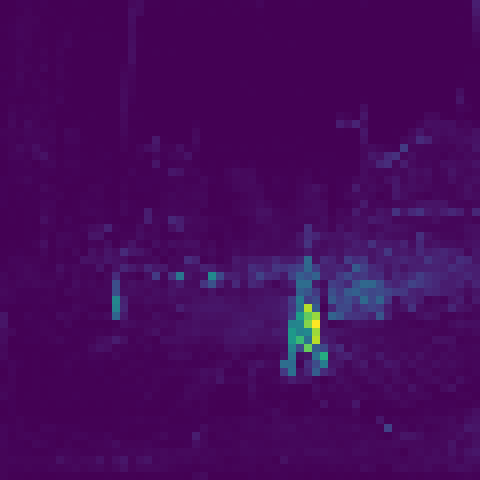
\includegraphics[width=\subfigwidth]{images/vit_attention/4/attn-head5.png}
    \end{subfigure} \\
\label{fig:attention_maps}
\end{tabular}
\end{figure}

\subsection{Data Preprocessing of Dr(eye)ve}
The Dr(eye)ve dataset is composed of 74 video sequences of five minutes each.
To reduce redundancy of images it was downsampled at 4 fps and resized and 
stretched to 300x300 pixels. Then RetinaNet \cite{retinanet} was used to detect 
the desired targets, 
and the label was assigned to the frame if at least one of the targets was detected.

Then we divided the dataset in training, validation and test sets. In particular,
the validation set is based on 1000 images, 
equally balanced between dangerous and safe situations.
The test set is based on 200 images, also equally balanced between dangerous 
and safe cases.
Both the validation and test sets are always kept fixed, with the same ratio.

On the other hand, the training set has different sizes, because we made some 
experiments in both supervised and semi-supervised learning, changing the 
labelled training size to figure out how it affected the predictions.
Therefore, we started with 500 labels, then 1000, 2500, 5000 and 10000.
The initial training set is not equally distributed between dangerous and safe 
cases (around 63\% of safe cases and 37\% of dangerous cases).
A further training set with 40000 labels was also made to better understand the 
model's behavior with a large amount of labelled data.

\subsection{Training Pipeline on Dr(eye)ve}
Starting from the smallest training set, when increasing labels after each 
experiment, we still use RetinaNet to classify new images. However, the criteria 
to augment the training set is based on the model's predictions. In particular, 
we used the object detector as a \emph{validator} to correct wrong predictions.
In summary, the training pipeline can be described in the following way:
%
\begin{algorithm}
    \nextfloat{\caption{Iterative training on the DR(eye)VE dataset}
    \label{alg:train_pipeline_dreyeve}}
    \vspace{0.2cm}
    \DontPrintSemicolon
    \text{Initialize training, validation and test sets} (\textbf{Algorithm \ref{alg:preprocessing}})\;
    \While{True}{
        \text{Train model in supervised or semi-supervised mode} (\textbf{Algorithm \ref{alg:pseudo_labelling}})\;
        \text{Update training set with $N$ wrong predictions} (\textbf{Algorithm \ref{alg:dataset_update}})\;
        }
\end{algorithm}
In particular, when increasing the training set, we compensate the unbalance 
between dangerous and safe cases by picking the same number of wrong predictions 
between the two classes. This is particularly useful to avoid the model to 
overfit on the majority class.
However, we also weight the loss function to give more importance to the 
minority class.

The same pipeline is used for training models with Meta Pseudo Labels, but in 
this case the unlabeled set is both used to train the model and to pick new 
samples to label. Moreover, we stopped the training when reaching the maximum 
validation accuracy of the student. 

\subsection{Data Preprocessing of BDD100k}
The BDD100K dataset is a large and diverse driving video database designed for 
the development and evaluation of automated driving technologies. It includes 
100,000 videos captured from various geographic, environmental, and weather 
conditions.
Each video in the BDD100K dataset is typically about 40 seconds long, recorded 
at 30 frames per second, resulting in approximately 1,200 frames per video. 
However, only 100,000 frames are completely labelled by humans, and each frame 
corresponds to the tenth second of a video.

Therefore, we used all the labelled frames and downsampled the unlabeled set (the 
videos) at 3fps. This is to reduce redundancy of data in semi-supervised 
learning and speeding-up the training process.
We also resized and stretched all frames to 600x600 pixels. We chose this 
resolution because it is a good trade-off between details of the scene and 
computational cost.

In this case it not required to use any validator because we only used 
human-labelled frames for the labelled training set. In particular, we labelled 
a frame as dangerous if there is at least one vulnerable target, including 
pedestrians, riders, bicycles. The scene is considered safe otherwise.
However, considering the trade-off between resolution and details described above, 
we choose to set a minimum threshold of the area occupied by the bounding box 
of the target to consider the scene as dangerous. This is particularly useful 
to have more reliable data, to make sure that the model is able to extract 
enough useful feature from.
The minimum threshold area is set to 5000 pixels for each target in the original 
image resolution of 1280x720 pixels.

\subsection{Handling Unbalanced Data}
Managing unbalanced datasets in binary classification poses significant challenges 
due to the disproportionate distribution of the classes. In such scenarios, 
models trained on these datasets might exhibit a bias toward the majority class, 
often at the expense of the minority class. This can lead to a situation where 
the model performs well statistically in terms of overall accuracy but fails to 
correctly identify instances of the less frequent class.

The complexity arises because the usual evaluation metric, accuracy, does not 
reflect the model's performance on the minority class effectively. 
This misrepresentation can lead to misleading conclusions about the model's true 
effectiveness, especially in the BDD100k dataset, where there is a proportion 
of 90\% of safe cases and 10\% of dangerous cases.

To address these challenges, it's crucial to employ a suite of metrics that 
provide a more comprehensive view of the model’s performance across both classes. 
Metrics such as precision, recall, F1-score, and others allow for a more detailed 
assessment of how well the model identifies and classifies instances from both the 
majority and minority classes. Each metric highlights different aspects of the 
model's behavior, such as its ability to correctly predict positive cases, avoid 
false positives, or balance these factors through a combined score. 
By considering these metrics, we can better understand 
and mitigate the biases inherent in models trained on unbalanced datasets.

\subsubsection{Evaluation Metrics}
In the context of unbalanced datasets like Dr(eye)ve and BDD100k, traditional 
accuracy, which simply measures the proportion of total correct predictions 
relative to the total dataset size, can be misleading. For instance, in BDD100k 
dataset, where 90\% of the data are of one class, a naive model predicting only 
that class would achieve 90\% accuracy, despite not having learned to identify 
the rarer class effectively.

Instead, more nuanced metrics such as precision, recall, and F1-score are used. 
Precision is the ratio of correctly predicted positive observations to the total 
predicted positives. It is defined as:
\begin{equation*}
    \text{Precision} = \frac{TP}{TP + FP}
\end{equation*}
where TP is the number of true positives and FP is the number of false positives. 
This metric helps to understand the accuracy of the positive predictions.

Recall (or sensitivity) measures the ability of a model to find all the relevant 
cases within a dataset. It is calculated by:
\begin{equation*}
    \text{Recall} = \text{Sensitivity} = \frac{TP}{TP + FN}
\end{equation*}
where FN is the number of false negatives. This metric is crucial for cases where 
missing a positive instance is significantly worse than falsely labeling negative 
instances as positive.

The F1-score is the harmonic mean of precision and recall, and is calculated by:
\begin{equation*}
    \text{F1-score} = 2 \times \frac{\text{Precision} \times \text{Recall}}{\text{Precision} + \text{Recall}}
\end{equation*}
This score is particularly useful for unbalanced datasets because it takes both 
false positives and false negatives into account, providing a more realistic 
measure of a model’s performance, especially when the classes are unevenly 
distributed.

In case of Dr(eye)ve this problem does not affect the validation set because it 
is forced to be balanced. However, the training set is unbalanced, and the model 
could overfit on the majority class, even though we also weighted the loss 
function. In this case, we used the F1-score as the main metric to evaluate the 
model's performance.

In case of BDD100k, on the other hand, the problem affects both the training 
and validation sets. In this case, we used the F1-score as the main metric to 
evaluate the model's performance. However, we also considered recall as an 
important metric to evaluate the model's ability to find all the relevant cases 
within the dataset, even though it could lead to more false positives.

\subsubsection{\ac{roc} Curve}
The Receiver Operating Characteristic (\ac{roc}) curve is a crucial tool for 
evaluating binary classification models, particularly in scenarios like detecting 
dangerous scenes in driving datasets, where the data is highly unbalanced. 
The ROC curve plots the true positive rate (sensitivity) against the false positive 
rate (1 - specificity) at various threshold settings. 
Sensitivity, as described above is also called recall, and specificity is 
defined as the true negative rate, or the proportion of negative instances 
correctly identified as such:
\begin{equation*}
    \text{Specificity} = \frac{TN}{TN + FP}
\end{equation*}


\begin{figure}
    \centering
    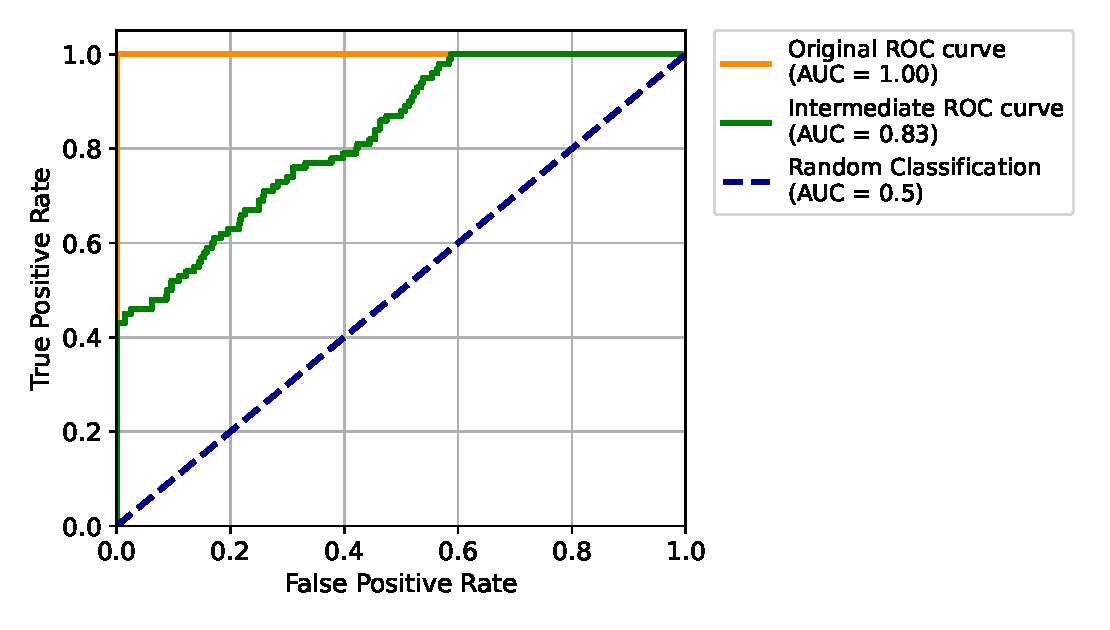
\includegraphics[width=0.95\textwidth]{images/roc/roc_curve.pdf}
    \caption
    {Example of ROC curve for a binary classification model.}
    \label{fig:roc_curve}
\end{figure}
This curve helps to 
visualize the trade-off between sensitivity and specificity from the two extreme 
operation points (with a threshold of 0.0 and 1.0).
In fact, it is possible to notice that setting a threshold of 0.0, the model 
will output all positive cases, then the sensitivity will be 1.0, but the 
specificity will be 0.0. On the other hand, setting a threshold of 1.0, the model 
will output all negative cases, then the specificity will be 1.0, but the 
sensitivity will be 0.0. An example of ROC curve is shown in Figure 
\ref{fig:roc_curve}.

Setting the operation point on the ROC curve involves choosing a specific 
threshold that defines how the binary classifier will categorize positive and 
negative classes. This threshold setting is crucial in unbalanced datasets 
because it helps balance the sensitivity and specificity according to the 
specific needs of the application. For instance, in detecting dangerous driving 
scenes, missing a dangerous scene (low sensitivity) might be more critical than 
incorrectly labeling a safe scene as dangerous (high specificity). Therefore, 
we choose a threshold that prioritizes sensitivity.

The optimal solution often depends on the specific costs associated with false 
positives and false negatives. These can be explicitly defined through a cost 
function, which quantifies the impact of these errors. For instance, a cost 
function could be constructed such that the cost of missing a dangerous scene 
(false negative) is set higher than incorrectly identifying a scene as dangerous 
(false positive). By minimizing this cost function across possible thresholds, 
we can determine the most cost-effective operation point on the ROC curve.

\subsubsection{\ac{mcc}}
The Matthews Correlation Coefficient (\ac{mcc}) is a metric used to evaluate the 
quality of binary classifications. It is especially useful in scenarios where 
the dataset is unbalanced. The MCC takes into account true and false positives 
and negatives and is generally regarded as a balanced measure that can be used 
even if the classes are of very different sizes. 
The coefficient returns a value between -1 and +1. An \ac{mcc} of +1 indicates a 
perfect prediction, 0 indicates a random prediction, and -1 indicates total 
disagreement between prediction and observation.
The formula for \ac{mcc} is:
\begin{equation*}
    \text{MCC} = \frac{TP \times TN - FP \times FN}{\sqrt{(TP + FP)(TP + FN)(TN + FP)(TN + FN)}}
\end{equation*}
When any of the sums in the denominator is zero, the denominator can be 
arbitrarily set to 1, leading to a \ac{mcc} of zero if both classes are absent 
from the dataset.

In unbalanced datasets, where the number of instances in each class is not equal, 
common metrics like accuracy can be misleading. For example, in a dataset where 
95\% of instances belong to one class, a model that always predicts the majority 
class will have high accuracy but will perform poorly on the minority class. 
The F1 score, which considers both precision and recall, improves on this by 
focusing on the performance related to the minority class but still can be skewed 
depending on the ratio of the classes.
\ac{mcc}, on the other hand, provides a more comprehensive evaluation as it 
considers all four confusion matrix categories, making it more reliable in 
assessing the performance of classifiers on unbalanced datasets.

Therefore, when evaluating the performance of supervised and semi-supervised 
learning on BDD100K, we combine multiple metrics, including \ac{roc} curve, 
\ac{auc}, F1-score and \ac{mcc}, to provide a comprehensive view of the model's 
effectiveness in detecting dangerous driving scenarios.
%
\chapter{Experiments}

\section{Traditional Computer Vision-based Approach}

\subsection{Glances to Vulnerable Users}
\begin{figure}
    \centering
    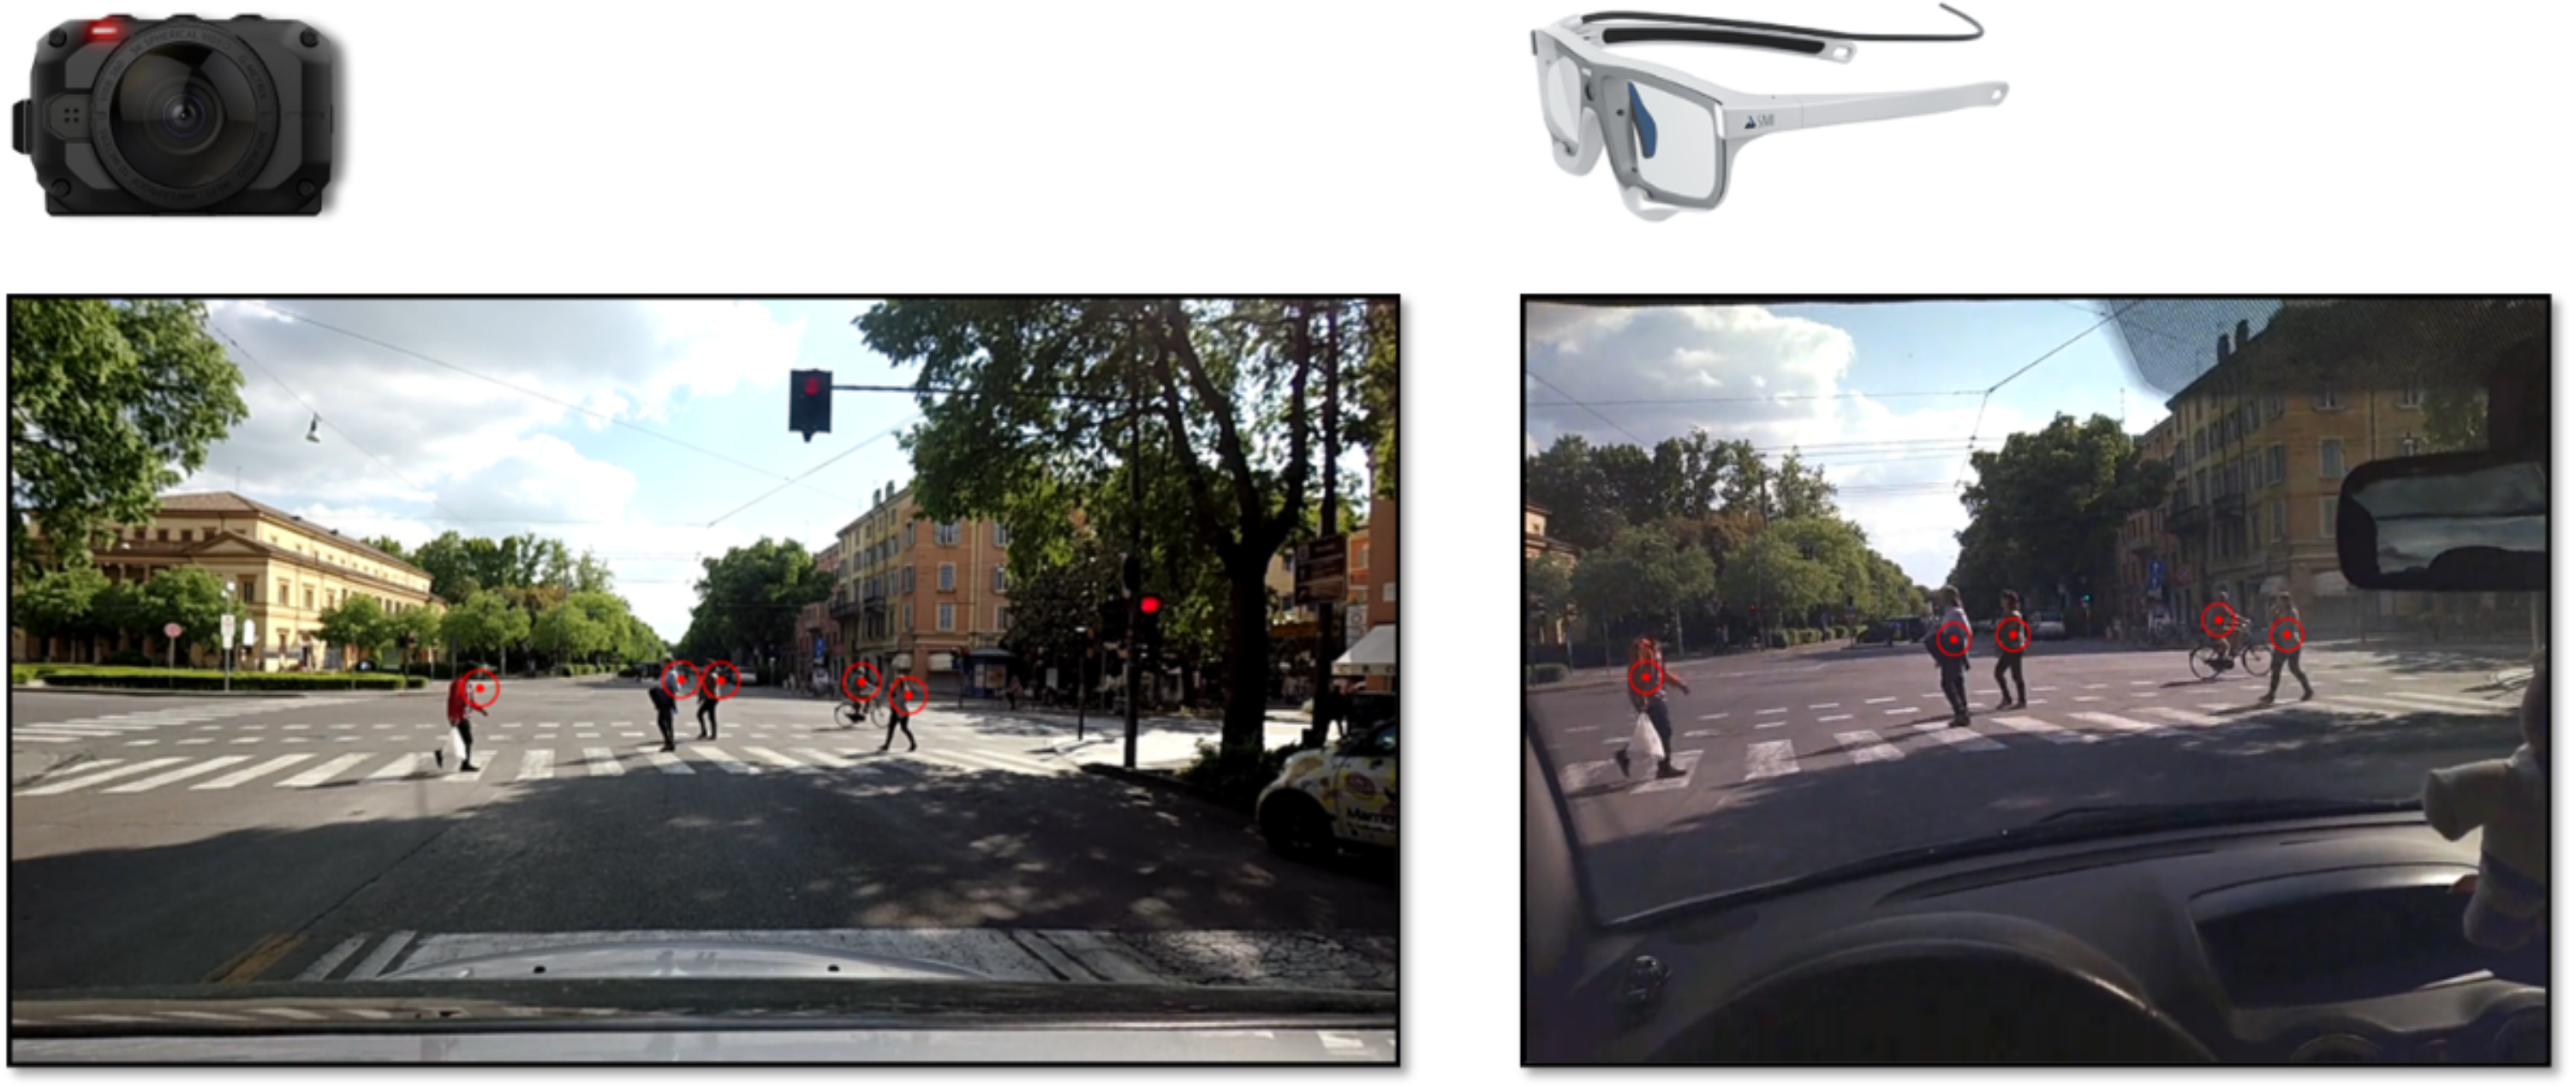
\includegraphics[width=\textwidth]{images/dreyeve/gaze_projection.png}
    \caption{Projection of the gaze from the ETG camera to the RT camera. 
    All the gaze points are manually set.
    \textbf{Left}: Roof top camera view.
    \textbf{Right}: ETG camera view.}
    \label{fig:gaze_projection}
\end{figure}
\begin{figure}
    \centering
    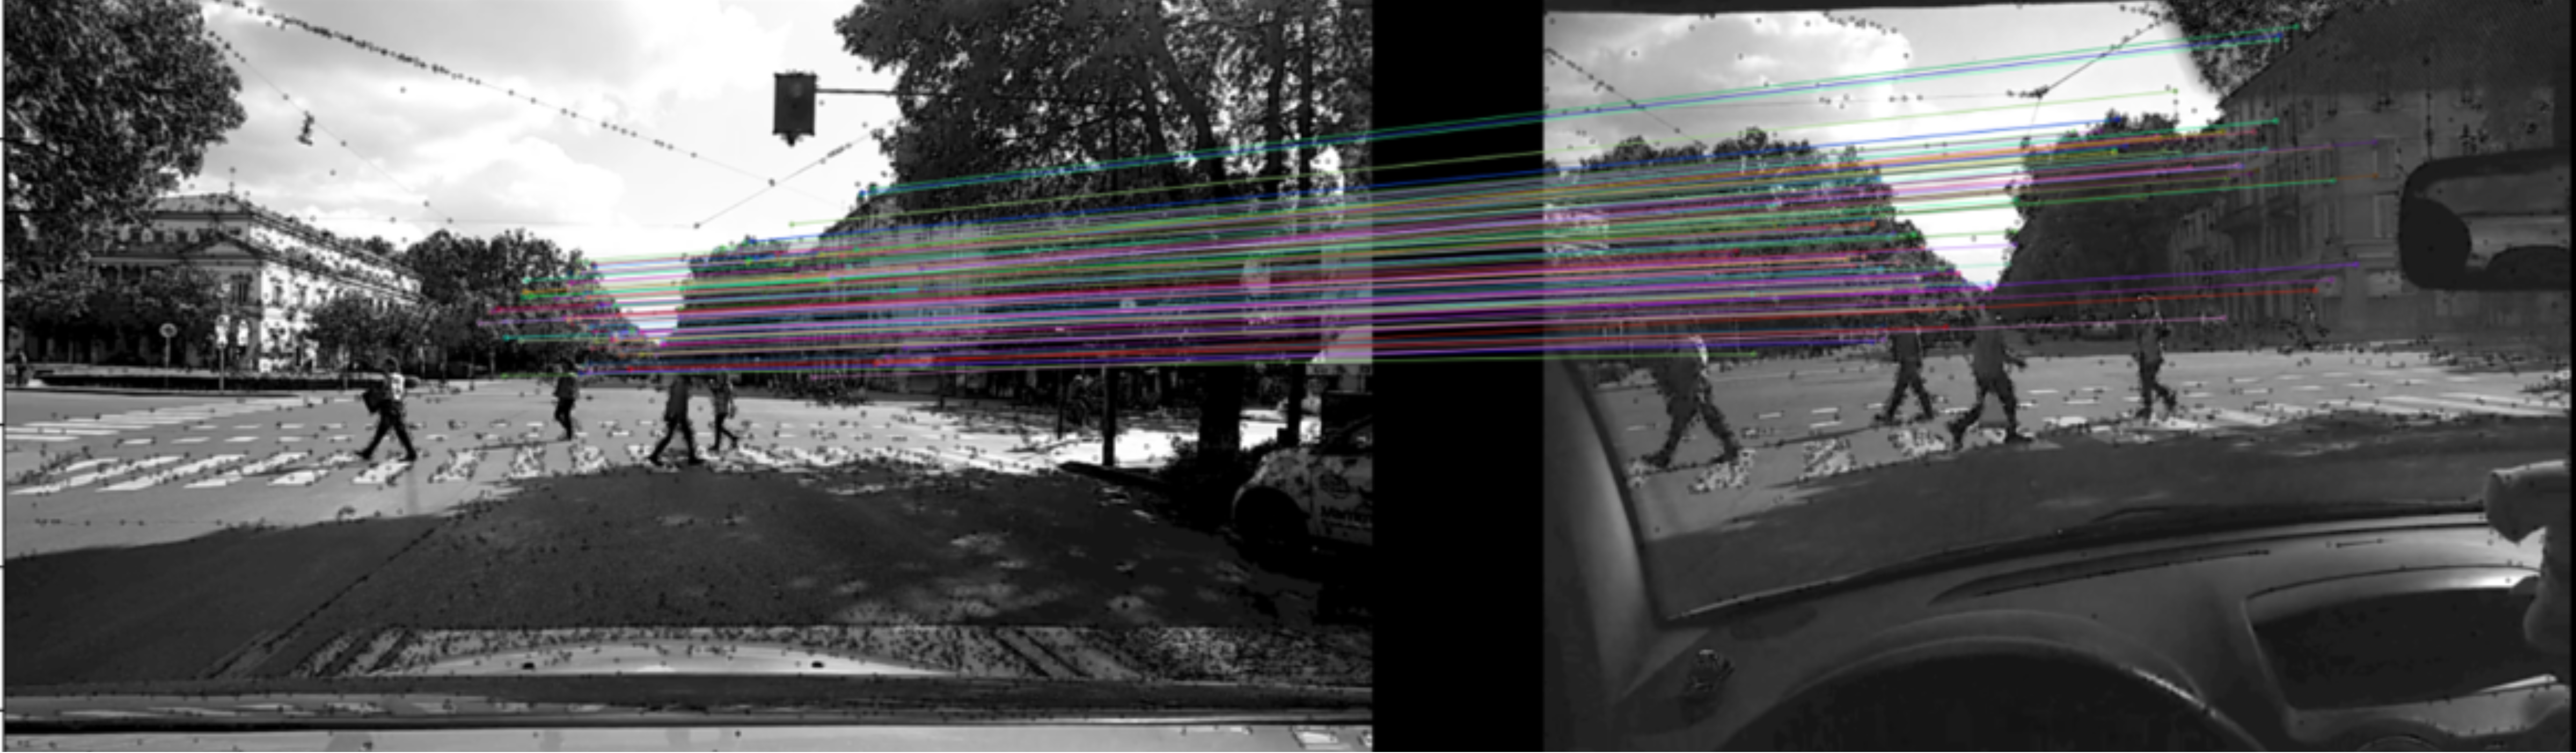
\includegraphics[width=\textwidth]{images/dreyeve/gaze_matchings.png}
    \caption{Projection of the gaze from the ETG camera to the RT camera. 
    All the gaze points are manually set.
    \textbf{Left}: Roof top camera view.
    \textbf{Right}: ETG camera view.}
    \label{fig:gaze_matchings}
\end{figure}
The projection of the gaze from the ETG camera to the RT camera is shown in 
Figure \ref{fig:gaze_projection}. We manually set some gaze points on the 
ETG camera such that they overlap with the vulnerable users. In this way, 
we are setting some operation points that we can use to evaluate the quality 
of the homography estimation. From the figure it is possible to see that the 
projection is not perfect, but it is a good approximation of the gaze in the 
RT camera plane. The small errors are due to the fact that the scene is not 
flat and the homography is a planar transformation. However, most pixels with 
high contrast correspond to objects that are far away from the vehicle, 
therefore the approximation is reasonable.

In Figure \ref{fig:gaze_matchings} we show keypoints' matchings between the 
two images. The keypoints are extracted using the SIFT algorithm.
In a first instance, matchings are computed according to the Lowe's ratio test, 
with a threshold of 0.7. This is to make sure that there is enough Euclidean 
distance from the best matching to the second best matching. Then, we apply 
the RANSAC algorithm, with a threshold of 5 pixels for the reprojection error.
Finally, we compute the homography matrix using the inliers from the RANSAC 
algorithm. To optimize the estimation problem, we set the maximum number of 
iterations to 2000 and a confidence of 99.5\%.

As it is possible to see from Figure \ref{fig:gaze_matchings}, the matchings 
are accurate enough to compute homography. The dark points are all the keypoints 
extracted with SIFT, and the colored lines are the correspondent matchings 
obtained through RANSAC. 
As expected, in a scenario wehre there is a high contrast between the road 
evironment and the sky, the matchings are related to those loactions. 
However, many other keypoints where there is high contrast are detected, for 
example on crosswalks, pedestrians and buildings. They are probably not matched 
beacuse they are not unique enough to satisfy the Lowe's ratio test.

This is a fundamental aspect to consider when designing a system that should be 
used in many different scenarios, during the day and night, in different weather 
conditions, etc. Moreover, in Figure \ref{fig:gaze_projection} and 
\ref{fig:gaze_matchings} we show the results of an especially favorable scenario, 
where there are good conditions of light and contrast, and the driver is looking 
straight ahead.

\subsection{Data Distribution of Dr(eye)ve}
After computing all the projected gaze points, we can focus on the interaction 
of the driver with the vulnerable users. Therefore, it is important to have 
a general overview of the distribution of people in the Dr(eye)ve dataset.
However, considering that the focus is on the interaction \emph{during time},
it is also important to embed poeple's tracking information in the analysis.

Therefore, in Figure \ref{fig:tracking_distribution} we count the number of 
different people that are tracked by the driver. In particular, on the lower 
x-axis there is the total observation time of the person in seconds. On the 
upper x-axis there is the number of frames where the person is tracked, this is 
just to have a different representation of the same data that considers 
preprocessing. On the y-axis there is the number of people observed by the driver 
for the specific amount of time. The distribution is shown in a logarithmic scale 
to better compare the values.
The plots also compare the downtown with all other scenarios. Green bars 
represent the downtown scenarios, while red bars represent the sum of all 
the scenarios in the dataset (therefore including the downtown).

The distribution is right-skewed, with a long tail of people that are observed 
for a short amount of time.
On one hand, this is expected, considering that the driver is usually looking 
straight ahead when driving. On the other hand, it is important to consider 
that some missing data could be due to tracking losses or occlusions with 
ByteTrack, or some non-accurate gaze projections that do not overlap with the 
bounding boxes of the people.

In Figure \ref{fig:tracking_cum_distribution} we show the cumulative distribution 
of the tracking counts. This is a useful representation to understand the number 
of people that are observed, and so tracked, for at least a certain amount of time. 
In this case, the y-axis is linear to better understand the variation of counts 
with respect to the time.

From the cumulative distribution it is possible to see that the total number of 
different observed people is around 110. However, considering a minimum observation 
threshold of 0.3s, which consists of 9 frames, the number of people is reduced 
to 40.
This is a relative small number to consider such a complex interaction betweeen 
humans, in many different scenarios. Moreover, as described in one of the next 
sections, ByteTrack suffers from some tracking losses and mismatching, 
compromising the quality of the data.

It is also important to consider the distribution of recordings with respect to 
time, weather and areas for each driver. In fact the Dr(eye)ve dataset is 
composed of 8 different drivers, each one with a different driving style and 
preferences. In Figure \ref{fig:dreyeve_rec_distrib} we 
show the mentioned plots. Data is enough equally distributed among the drivers, 
with a slight preference for some of them. This means that the behavioral 
information embedded in the dataset can generalize well.

\begin{figure}
    \centering
    \begin{minipage}{0.49\textwidth}
        \centering
        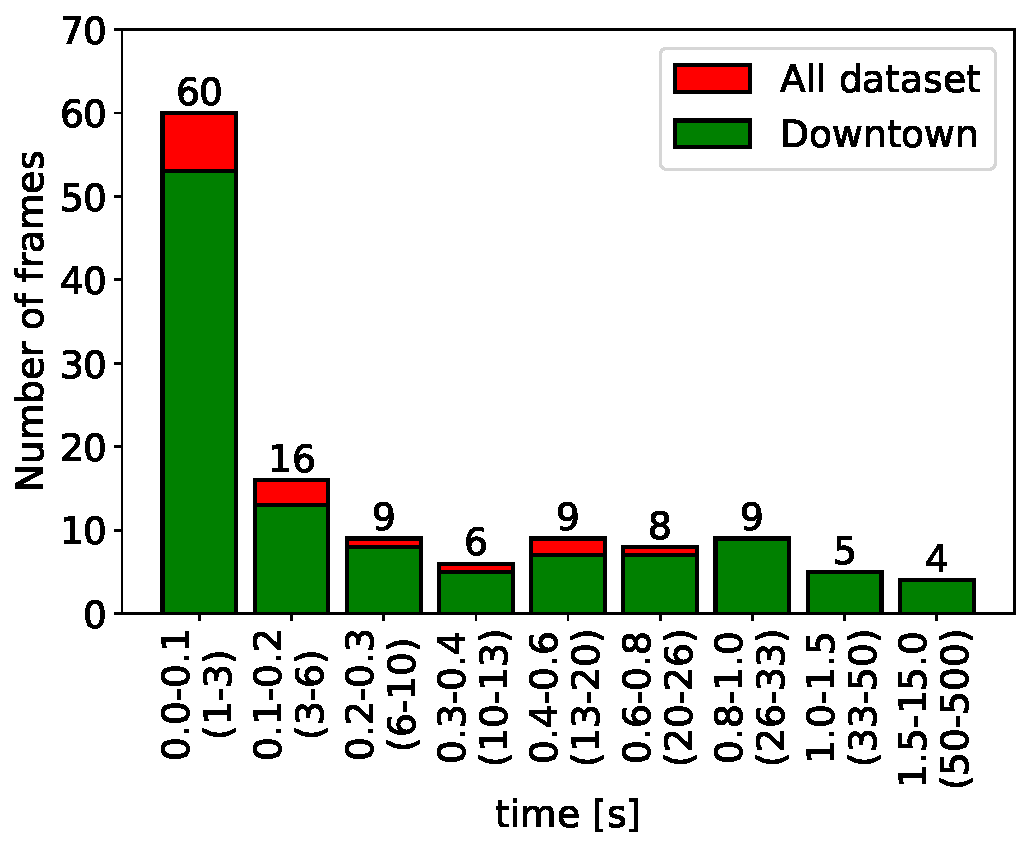
\includegraphics[width=\textwidth]{images/dreyeve/tracking_distrib.pdf}
        \caption{Observation time counts.}
        \label{fig:tracking_distribution}
    \end{minipage}\hfill
    \begin{minipage}{0.49\textwidth}
        \centering
        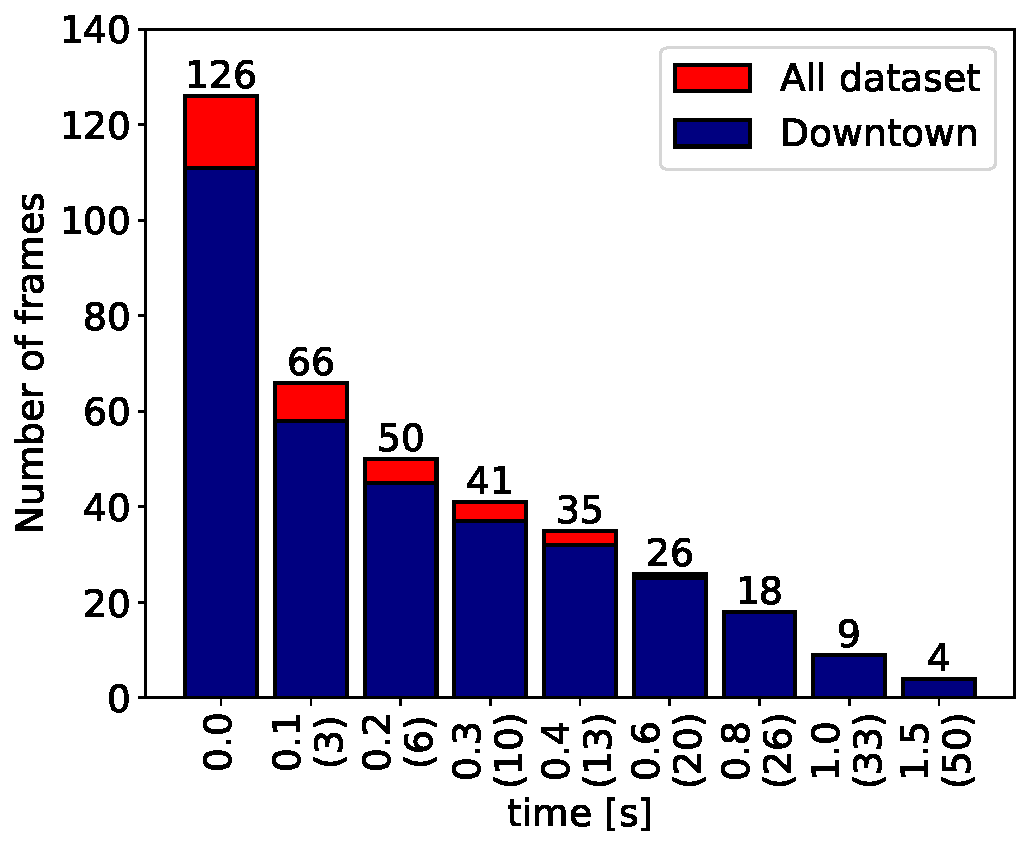
\includegraphics[width=\textwidth]{images/dreyeve/tracking_distrib_cum.pdf}
        \caption{Cumulative of the counts.}
        \label{fig:tracking_cum_distribution}
    \end{minipage}
\end{figure}


\begin{figure}[h]
    \centering
    \begin{minipage}{0.33\textwidth}
        \centering
        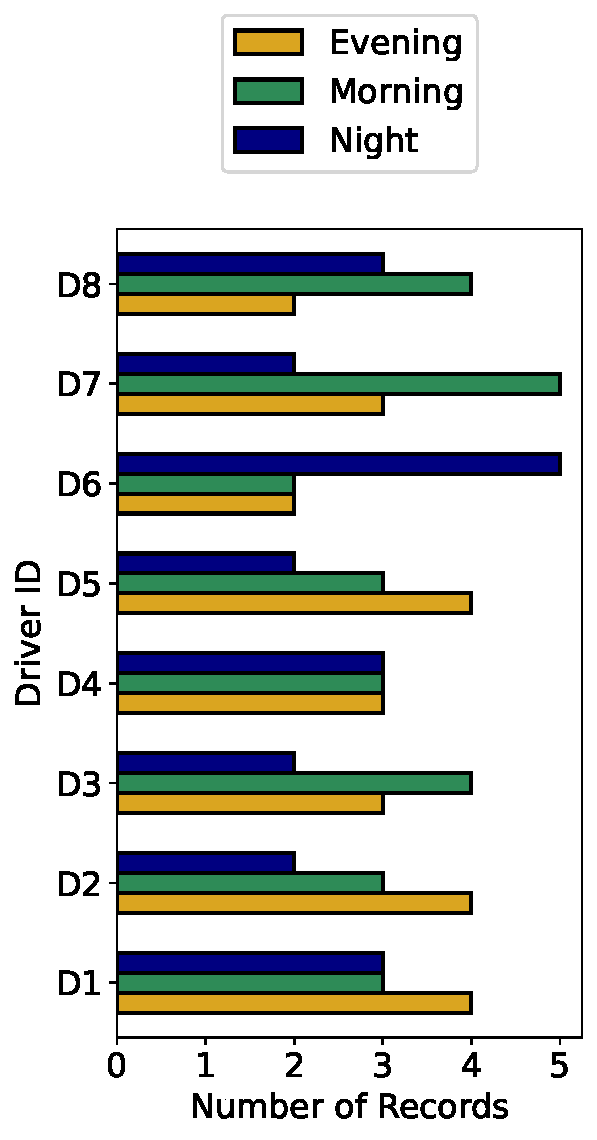
\includegraphics[width=\textwidth]{images/dreyeve/time_distrib.pdf}
    \end{minipage}\hfill
    \begin{minipage}{0.33\textwidth}
        \centering
        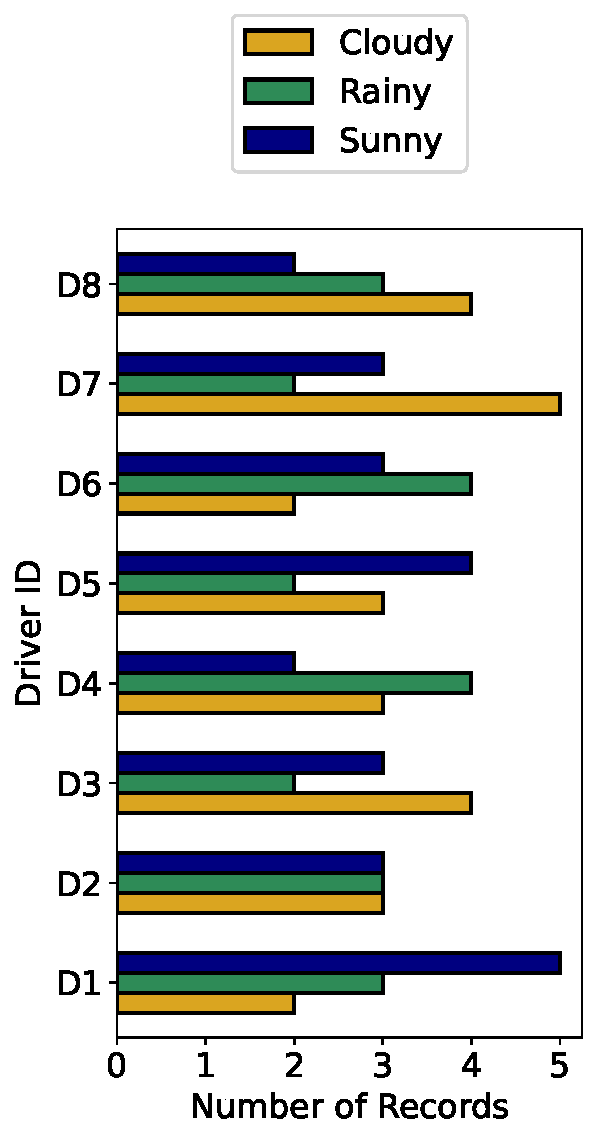
\includegraphics[width=\textwidth]{images/dreyeve/weather_distrib.pdf}
    \end{minipage}\hfill
    \begin{minipage}{0.33\textwidth}
        \centering
        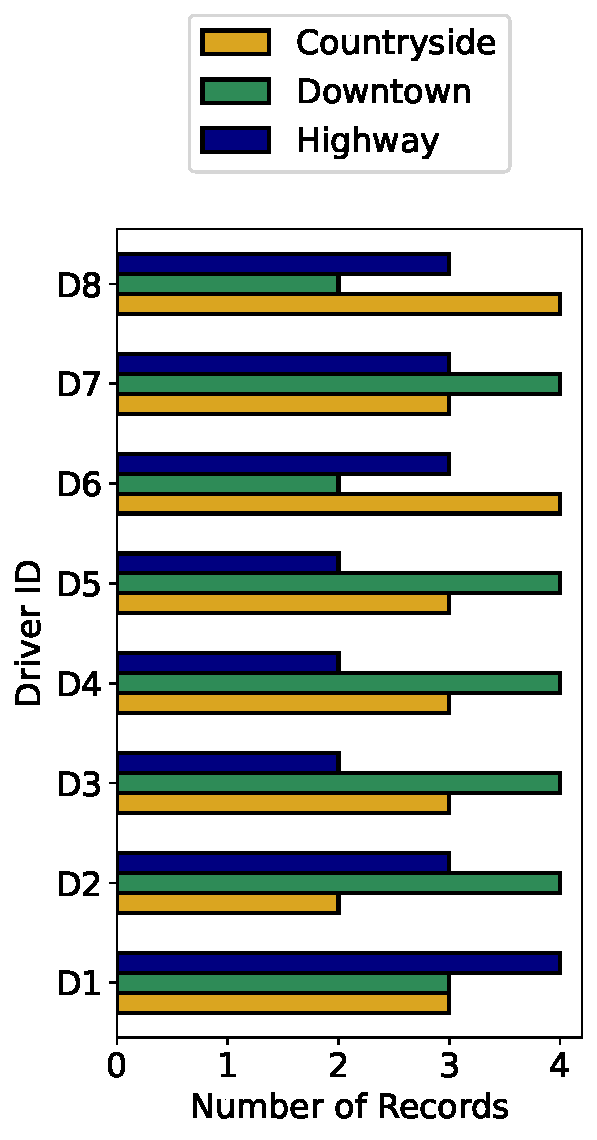
\includegraphics[width=\textwidth]{images/dreyeve/area_distrib.pdf}
    \end{minipage}\hfill
    \caption{Distribution of recordings in Dr(eye)ve dataset. 
    \textbf{Left}: Distribution of recordings with respect to time.
    \textbf{Center}: Distribution of recordings with respect to weather.
    \textbf{Right}: Distribution of recordings with respect to driving areas.}
    \label{fig:dreyeve_rec_distrib}
\end{figure}

\subsection{Gaze Interaction with Targets}
In Figure \ref{fig:glances} there are six different people that the driver 
observed for at least 0.5 seconds. This minimum threshold is considered a good 
compromise between the time needed to understand the context and the quantity 
of data available, as shown in Figure \ref{fig:tracking_cum_distribution}.
Each plot is referred to a unique person, tracked during the whole sequence.
In particular, it is possible to notice that two different functions overlapped
for each plot:
the observation signal (blue) and the detection signal (red).
Both functions can assume two different states: True or False.

The observation signal is set to True when the driver is looking at the person, 
and False otherwise. The detection signal is set to True when the person is 
correctly detected and tracked by ByteTrack; otherwise it is set to False.
Therefore we can have three different states:
\begin{itemize}
    \addtolength\itemsep{-2mm}
    \item \textbf{D=True, O=True}:\\
    Driver is looking at a visible and detected person.
    \item \textbf{D=True, O=False}:\\
    The person is visible and detected, but the driver is not looking at it.
    \item{\textbf{D=False, O=False}}:\\
    Tracking of person is lost (possible overlapping, occlusion or missed detection).
\end{itemize}
It is important to emphasize that it is not possible to also have the fourth state 
with D=False and O=True, even though the driver could be looking at a person that 
is not detected by ByteTrack at the moment. Therefore, when there are high 
variations of both the observation and detection signals at the same states, 
it is possible that the person is occluded or overlapped, and the driver is 
looking at it. If the frequency is very high, probably the detection algorithm 
is missing some detections between time frames (e.g. there is a variation of 
light conditions, some quick movements, etc.). An example of this case is shown 
in Figure \ref{fig:glances}.d), between 11s and 13s.

Another case is when the person is continuously detected and the driver is looking 
at it only for a short period of time. There can be oscillations of the observation 
during this period, probably due to a small projection error when the case is close 
to some corners of the bounding boxes. This can be amplified in quick movements' 
scenarios. An example of this case is shown in all the figures in different 
periods of time.

If the person is detected continuously and the observation signal varies slowly 
and periodically, like in Figure \ref{fig:glances}.b-e), it is possible that the 
driver is looking at different parts of the scene keeping updating the attention 
towards them.

Finally, in Figure \ref{fig:glances}.c-f) there are some cases where the person 
is not glanced at by the driver, and the detection signal varies at high 
frequency. This is the case when the person is visible and tracked, but the driver 
is not paying attention to it. 

This is a good example of the importance of contextualizing the scene through 
perception and driver's data. However, there are many complex cases that are 
difficult to explain with just these two signals, especially when it is 
fundamental to consider possible tracking losses or mismatchings.

\begin{figure}
    \raggedright
    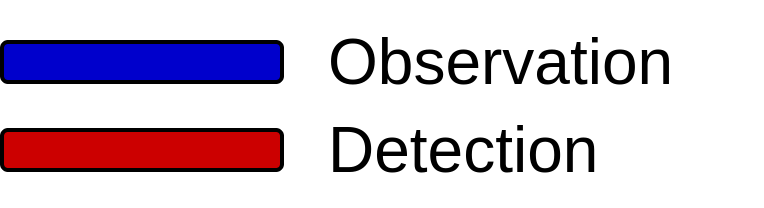
\includegraphics[width=0.23\textwidth]{images/dreyeve/gazes/glances_legend.png}\\
    \centering
    \begin{minipage}{0.5\textwidth}
        \centering
        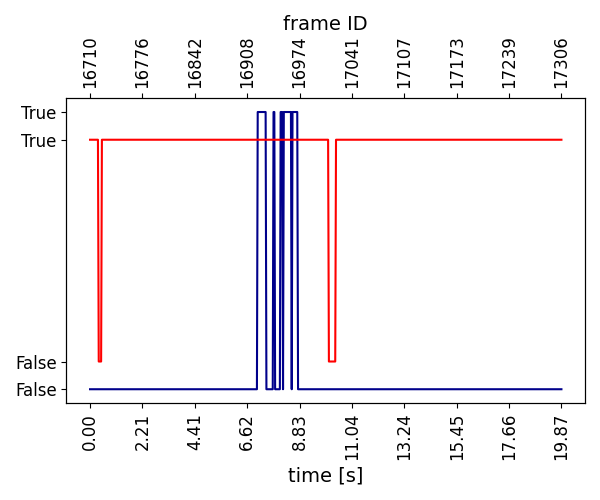
\includegraphics[width=\textwidth]{images/dreyeve/gazes/1.png}
        \textbf{a)}
    \end{minipage}\hfill
    \begin{minipage}{0.5\textwidth}
        \centering
        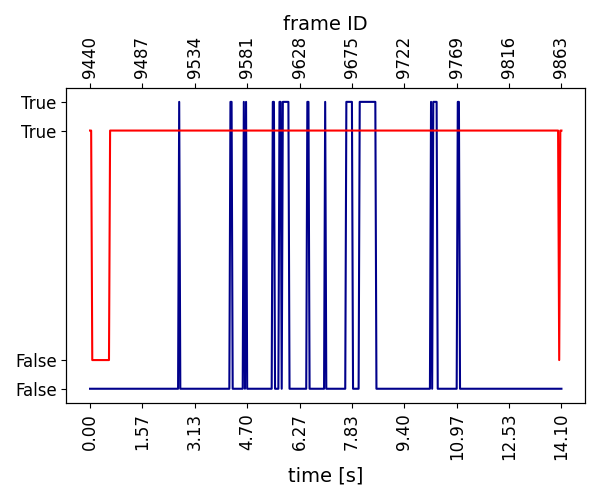
\includegraphics[width=\textwidth]{images/dreyeve/gazes/2.png}
        \textbf{b)}
    \end{minipage}\hfill \\\vspace{0.2cm}
    \begin{minipage}{0.5\textwidth}
        \centering
        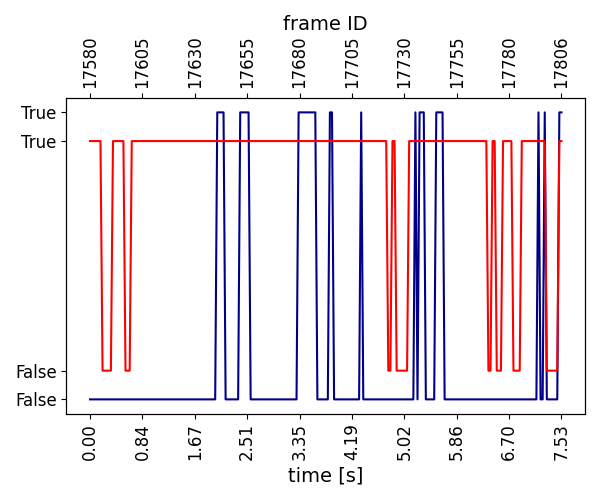
\includegraphics[width=\textwidth]{images/dreyeve/gazes/3.png}
        \textbf{c)}
    \end{minipage}\hfill
    \begin{minipage}{0.5\textwidth}
        \centering
        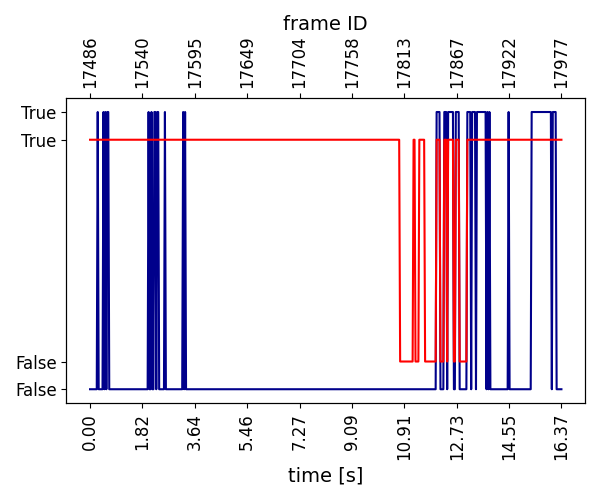
\includegraphics[width=\textwidth]{images/dreyeve/gazes/4.png}
        \textbf{d)}
    \end{minipage}\hfill\\\vspace{0.2cm}
    \begin{minipage}{0.5\textwidth}
        \centering
        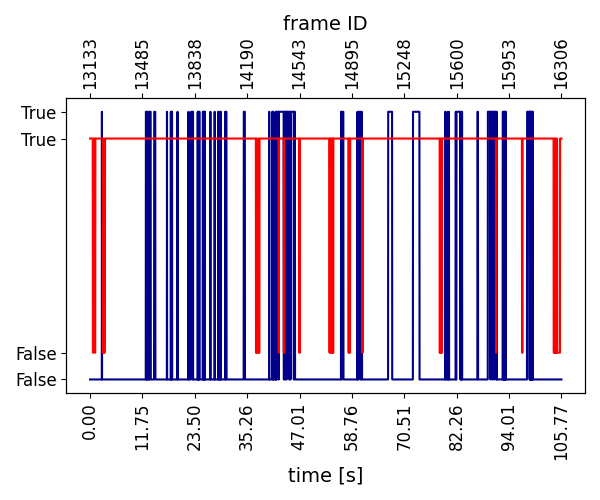
\includegraphics[width=\textwidth]{images/dreyeve/gazes/5.png}
        \textbf{e)}
    \end{minipage}\hfill
    \begin{minipage}{0.5\textwidth}
        \centering
        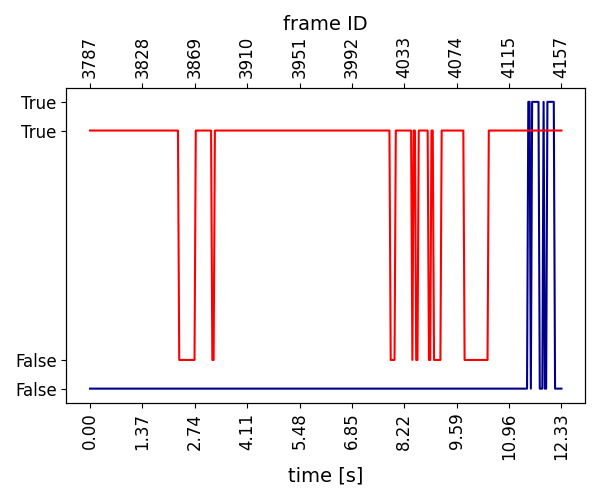
\includegraphics[width=\textwidth]{images/dreyeve/gazes/6.png}
        \textbf{f)}
    \end{minipage}
    \caption{Driver glances towards people in the Dr(eye)ve dataset 
    (minimum glance threshold is set to 0.5s).}
    \label{fig:glances}
\end{figure}

\subsection{Tracking Performance}
As mentioned before, analyzing driving interatctions between the driver and 
vulnerable users is a complex task that can be compromised by tracking errors.
Even though ByteTrack is a state-of-the-art tracking algorithm, especially 
designed for scenarios with occlusions and overlapping, it can still suffer 
from some mismatches and tracking losses.
It is complicated to find out when the tracking is lost, from the output of 
the algorithm. Even worse, if there is a tracking mismatch, driver's gaze 
information can be compromised, leading to wrong conclusions about the interaction 
between the driver and the other targets.

In Figure \ref{fig:tracking_mismatch} we show some examples of tracking mismatches
in a driving scenario of Dr(eye)ve.
In particular, four different frames from the roof top camera are shown. 
We decided to show the frames where there are overlapping or occluded people, 
to emphasize the complexity of the tracking task.

From Figure \ref{fig:tracking_mismatch}.a) to Figure \ref{fig:tracking_mismatch}.b)
the tracked person (with ID 342) overlaps with another person that is walking on 
the crosswalks. In this case the tracking is not lost, and the person is correctly 
tracked.

From Figure \ref{fig:tracking_mismatch}.b) to Figure \ref{fig:tracking_mismatch}.c)
the same tracked person overlaps with another target, but this time there is 
a tracking mismatch. The bounding box is now assigned to the incoming person, 
and the tracked person is lost.

A similar case is shown from Figure \ref{fig:tracking_mismatch}.c) to 
Figure \ref{fig:tracking_mismatch}.d). The tracked person is mismatched with 
another incoming person.

Even though lighting conditions are optimal, and people are not occluded by 
other objects, tracking mismatches can still happen. This is a fundamental 
aspect to consider when designing a feature for an ADAS system. 
Another aspect is that, despite the presence of other objects in the background 
like cars, the tracking algorithm is able to correctly keep the right tracking, 
considering that the backbone model is not specifically trained on detecting 
people in driving scenarios. This is a good sign of the robustness of the 
algorithm with respect to the background environment, and could be enhanced 
through an ad-hoc fine-tuning of the detection stage on driving scenarios.
\begin{figure}
\centering
\includegraphics[width=0.85\textwidth]{images/dreyeve/tracking_mismatch.png}
\vspace{0.4cm}
\caption{ByteTrack's tracking mismatches in a driving scenario.}
\label{fig:tracking_mismatch}
\end{figure}

\subsection{Monocular Depth Estimation with MiDaS}
In this section we show and evaluate the results of the monocular depth estimation 
computed by MiDaS \cite{midas}. To evaluate the quality of the estimation it 
is necessary to have a ground-truth information to compare with. In this case, 
Dr(eye)ve dataset does not provide any depth information by default, because no 
depth sensors are used. 
Therefore, the idea is to validate the model on another 
dataset that provides depth information and a good variety of scenarios, from 
downtowns to highways, with different weather conditions, etc. 
We decided to use the NuScenes dataset \cite{nuscenes}, that provides both 
LiDAR and camera data.

\subsubsection{Evaluation on NuScenes}
In Figure \ref{fig:mde} we show the results of the monocular depth estimation 
for an entire scene of the NuScenes dataset. The left image is an heatmap of 
the relative inverse depth estimated by MiDaS, and compared with the ground-truth 
pointclouds taken from the front LiDAR. In particular, it is necessary to mention 
that MiDaS provides a \emph{relative} inverse depth that depends on the specific 
image, depending on the distance of closer and farther objects.
Considering that the comparison is not straightforward for the entire dataset, 
we decided to show the results for one entire scene, where at least the same 
environment is present in all the frames. Then the relative inverse depth is 
normalized to be in the range $[0, 1]$, and compared with the absolute depth 
of correspondent points in the LiDAR pointcloud. This means that non-correspondent 
pixels in the dense depth map are masked out.
Finally, we decided to use an heatmap to not only show the distribution of points, 
but also find how frequently the model makes some errors in the estimation.
Considering the preprocessing of the data, a reference curve is also shown. 
It spans from 4m to 60m on the x-axis and from the 
minimum to the maximum of the relative inverse depth on the y-axis. This is to have 
a unique function that is able to map all values in the two domains.
To be precise, the reference curve should not span only up to the maximum 
value of the pointcloud, but it should consider the maximum distance in the 
entire scene. However, this is a good approximation to have a general idea 
of the quality of the estimation, leveraging ground-truth data. In fact, 
from the experiments we realized that the model is more accurate in estimating 
high relative distances between objects in the scene, and this is usually related 
to closer-to-the-ego-vehicle objects. Moreover, LiDAR pointclouds can reach 
up to 100m, but the further points are, the more sparcely they are distributed
in the 3D space.

Another important aspect to consider is the output of MiDaS, that is the relative 
inverse depth. This means that the closer the object is, the higher the output 
of the model is. This is the opposite of the LiDAR pointcloud, where the closer 
the object is, the lower the depth value is. However, we decided not to invert 
one of the two signals to have a better comparison at closer distances, but also 
including farther estimations, with the output tending to zero for the farther objects.

From the results in the heatmap it is possible to notice that the model is able 
to estimate the depth of closer objects with a good approximation, but it is 
much less accurate for farther objects. Regarding closer objects, there 
are many point clouds related to the road that, considering its shapes, it is 
probably easier to estimate. On the other hand, farther objects are usually 
less visible in the image, and the model is not able to estimate them correctly. 
Moreover, there are some close pointclouds that are estimated far from the ego-vehicle,
and it adds a consistent error for the evaluation.

\subsubsection{Relative Evaluation Metrics}
Considering the problems to evaluate the accuracy of the model with respect to 
the ground-truth data, we decided to report two error metrics: the root mean 
squared error (RMSE) and the relative root mean squared error (RRMSE). 
They are calculated as follows:
\begin{align}
    \text{RMSE} = \sqrt{\frac{1}{n} \sum_{i=1}^{n} \left(d_i - \hat{d}_i\right)^2} \qquad\qquad
    \text{RRMSE} = \sqrt{\frac{1}{n} \frac{\sum_{i=1}^{n}{\left(d_i - \hat{d}_i\right)^2}}{\sum_{i=1}^{n}d_i^2}} \nonumber
\end{align}
where $d_i$ is the normalized depth of the i-th point in the LiDAR pointcloud, 
and $\hat{d}_i$ is the relative depth estimated by MiDaS. In total 
there are $n$ point clouds visible in the scene. As it possible to notice from the 
definition of the metrics, the RRMSE is a normalized version of the RMSE with 
respect to the average depth of the scene. This is useful to understand the 
quality of the estimation in all the dataset. However, we have inverted the 
relative depth obtained from MiDaS, therefore small values in the dense depth 
map heavily affect the RRMSE.

The right image, on the other hand, 
shows the projection of the LiDAR pointcloud on the image plane, through the 
camera calibration matrix. Each point is colored according to the depth value 
in the LiDAR pointcloud. This is to have a visual understanding of the distribution 
of pointclouds in one frame of the scene. As shown in the picture, the scenario 
corresponds to a downtown environment, with many buildings and cars. 
Closer point clouds can be related to the road, parked vehicles on the sides, 
road obstacles, etc. Farther point clouds are usually related to buildings, 
trees, and other objects that are not directly on the road.
\begin{figure}
    \centering
    \begin{minipage}{0.52\textwidth}
        \centering
        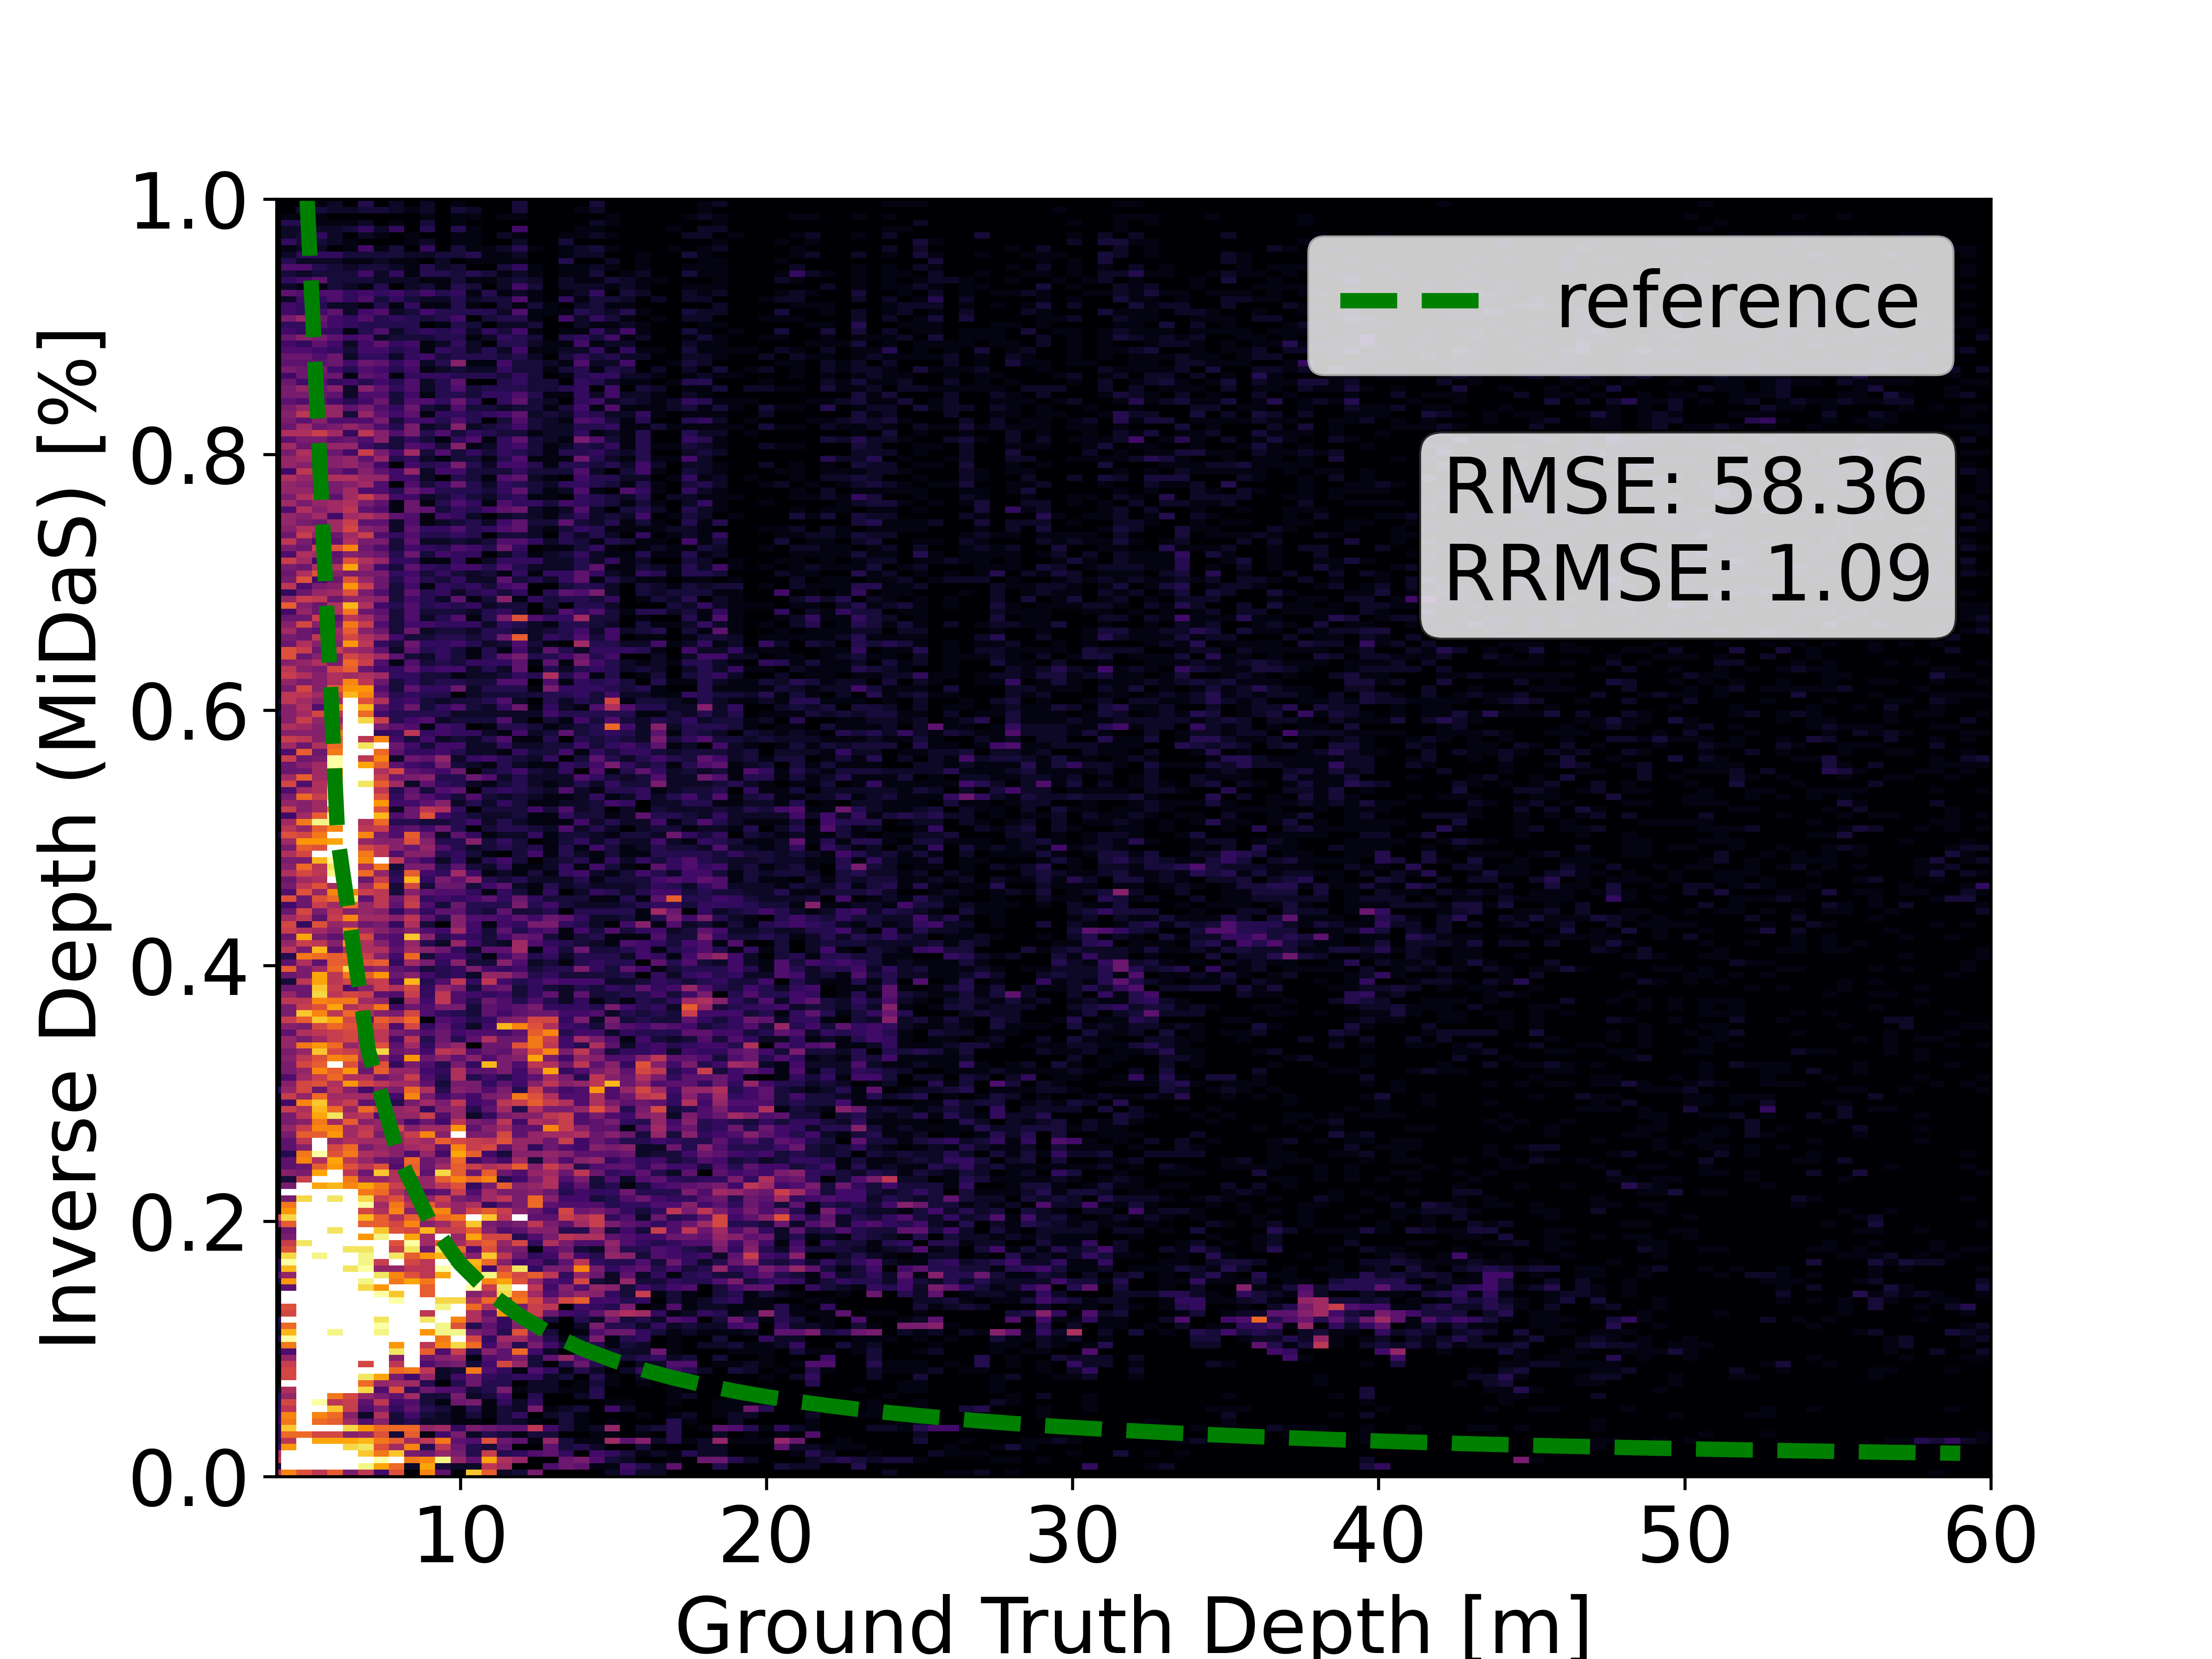
\includegraphics[width=\textwidth]{images/nuscenes/depth_0.png} % first figure itself
    \end{minipage}\hfill
    \begin{minipage}{0.47\textwidth}
        \centering
        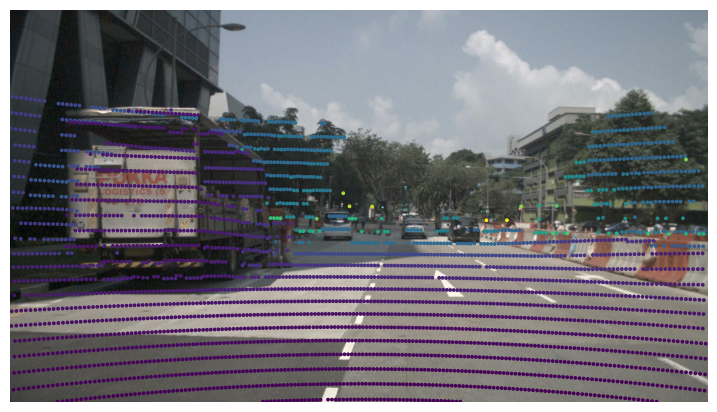
\includegraphics[width=\textwidth, height=4.8cm]{images/nuscenes/lidar_over_img.png} % second figure itself
    \end{minipage}
    \caption{Monocular depth estimation with MiDaS on NuScenes dataset \cite{nuscenes}.
    \textbf{Left}: Relative inverse depth estimated from the model compared to 
    the ground-truth information taken from the front LiDAR for an entire scene.
    \textbf{Right}: Projection of the LiDAR point cloud on the image plane for
    one sample of the same scene.} 
    \label{fig:mde}
\end{figure}

After having introduced the relative metric, the RRMSE, we evaluated the model 
on other five scenes of the dataset. Results for camparing the metrics are reported in 
Table \ref{tab:mde_metrics}.
\begin{table}[h]
    \vspace{0.3cm}
    \centering
    \begin{tabular}{ccc}
    \hline
    \textbf{Scene} & \textbf{RMSE} & \textbf{RRMSE} \\ \hline\hline
    Scene 1 & 58.36 & 1.09 \\ \hline
    Scene 2 & 29.09 & 0.52 \\ \hline
    Scene 3 & 26.50 & 0.53 \\ \hline
    Scene 4 & 21.96 & 0.40 \\ \hline
    Scene 5 & 24.54 & 0.99 \\ \hline
    \end{tabular}
    \caption{Evaluation of MiDaS on five scenes.}
    \label{tab:mde_metrics}
\end{table}



\section {Deep Learning-based Approach}
\subsection{Training on Dr(eye)ve}
To compare supervised and semi-supervised training of ViTs on Dr(eye)ve, we 
trained different models with different number of labels. In particular, we 
used the method with the validator explained in the methods section.
The reason behind using two different vision transformer models is to also 
understand if and when more parameters are necessary to better generalize the 
validation set.

In Table \ref{tab:dreyeve_training} we show the results obtained with the 
training method for both supervised and semi-supervised training.
Relevant information to track is reported in the columns, and they are:
\begin{itemize}
    \addtolength\itemsep{-2mm}
    \item \textbf{Mode}: the training method used, supervised or semi-supervised
    (MPL).
    \item \textbf{Model}: the vision transformer model used, MViT or LViT.
    \item \textbf{Labels}: the number of labels used in the training.
    \item \textbf{Safe [\%]}: the percentage of safe frames in the training set.
    \item \textbf{Dang. [\%]}: the percentage of dangerous frames in the training set.
    \item \textbf{top-acc.}: the best accuracy of the model on the validation set.
    \item \textbf{Biters @top-acc.}: the number of batches seen by the model when 
    it reaches the top accuracy.
    \item \textbf{max. Biters}: the maximum number of batches seen by the model 
    during the entire training.
\end{itemize}
In Table \ref{tab:models_dreyeve} the two models, MViT and LViT, are described 
in details through their fundamental hyperparameters. In order, they are:
\begin{itemize}
    \addtolength\itemsep{-2mm}
    \item \textbf{Patch size}: the dimension of each patch in pixels.
    \item \textbf{Emb. size}: the size of the embedding layer.
    \item \textbf{Depth}: the number of layers in the model.
    \item \textbf{Heads}: the number of heads in the multi-head attention mechanism.
    \item \textbf{MLP size}: the size of the multi-layer perceptron of the model.
\end{itemize}

\subsubsection{Training Setups}
Regarding the trainings, we used a learning rate of 0.001, a seed of 42, and 
two GPUs' setups: one with two NVIDIA Tesla A100 of 40GB each, and the other with 
one NVIDIA RTX 3080 of 10GB. The semi-supervised learning was performed in the 
first setup, in distributed training. The supervised learning, on the other hand, 
was performed in the second setup. 

Considering different models, different setups and different 
training methods, we introduce a custom metric, \emph{Biter}, that allows to 
compare the results in all the experiments. The metric defines the number of 
batches that the model has seen during training, therefore it is calculated as 
the batch size multiplied by the number of iterations. This is a good metric 
for comparing supervised and semi-supervised training because it is independent 
from the number of labels used. This is important, considering that while Meta 
Pseudo Labels iterates through the labelled dataset it also add new information 
from the unlabelled dataset. Therefore, the number of epochs has a different 
meaning in the two training methods.

\subsubsection{Training Results}
From the results in Table \ref{tab:dreyeve_training} it is possible to notice 
that in supervised learning mode the model asymptotically increases the best 
accuracy with the number of labels. This is expected, considering that the 
model is able to generalize better with more information. However, the model 
does not always increase the accuracy with the number of labels, as shown in 
the case of MViT-1k and MViT-5k. This is probably due to the fact that adding 
more labels does not always mean better generalization. In fact, some new labels 
could just be already seen samples, contributing to unbalancing the dataset with 
respect to the validation set. 

For the supervised training, from 500 to 5,000 labels, Biters to reach the top
accuracy increase exponentially, until 100,000 Biters for the last case, 
due to the increasing size of the labelled set.
However, with many more labels, the case with 40,000 labels, just 36,000 Biters 
are required to reach the optimal training. This is probably due to the redundancy 
of the labels that comes when substantially enlarging the dataset.


The experiment with 40,000 labels was specifically design to understand the model 
behavior with a large amount of labels. What we noticed is that the model 
overfits the training set in all the cases except for the last one. This is 
why we also decided to train the LViT model with 500 and 10,000 labels.
In the former case, it is possible to notice that with more parameters the model 
reaches better generalization with respect to the MViT model with the same number 
of labels. In the latter case, the model still increases the best accuracy with 
respect to both the MViT and LViT models with less labels. This implies that 
increasing the model is beneficial also with few labels.

Regarding the semi-supervised training with 500 labels, the model is able to 
outperform all the supervised epxeriments up to 5,000 labels. This is a good 
result, considering that the smaller model in semi-supervised learning performs 
similarly to the larger model with 20 times more labels. This means that 
unlabelled data carries a lot of information that can be used to improve the 
generalization of the model.
However, when training in semi-supervised learning mode, it is complicated 
to understand when the model is overfitting the labelled set. This is because 
training is done in two stages for each iteration, through the teacher and the 
student. Therefore, for a range of Biters, the teacher is learning the training 
set to better supervise the student. During the second phase, the student 
starts learning from the "right" pseudo-labels, better performing the teacher 
on validation data.
This process takes many more Biters than the supervised learning, as it is 
possible to notice in the last column of Table \ref{tab:dreyeve_training}.
However, a validation accuracy of 0.77 is reached with just 180,000 Biters.

\subsubsection{Models Description}
The patch size is kept at 6 pixels, considering that the dataset is based on 
images with a resolution of 300x300 pixels. This means that each image is 
divided in 50x50 patches; this seems a good compromise to both have a general 
overview of the scene and to have enough information to understand the details.

On the other hand, embedding size is increased from 64 to 1024, considering the 
quantity of information to keep to represent the complexity of the dataset.
The depth of the model is increased from 6 to 14, and the number of attention 
heads is doubled. This is to let the model learn more complex and deep features, 
with many relations between the patches. Finally, the size of the multi-layer
perceptron is increased to 2048, to better match extracted features with 
dangerous scenarios.


\subsubsection{Possible Problems}
We also made one last experiment in supervised learning, substantially reducing 
the transformer's size. In this case, the model overfits quickly the training 
set, in both cases with few and many labels, without reaching the same generalization of 
the other cases. This strange behavior is probably due to the fact that the 
model is not able to learn the complexities of the dataset with a smaller 
number of parameters. The quick overfitting can be justified by easier, but 
wrong, features extracted by the model.

However, there is a potential problem in the training pipeline; the training 
and validation sets are not related to completely different scenes. This means 
that some frames of the same video can be in the training set and in the 
validation set. Even though the frames are not the same, and videos were 
downsampled at 4Hz, there still could be some information leakage between the 
two sets. 

These are a fundamental aspects to consider, and that is also why we 
decided to move to BDD100k for the next experiments. Moreover, BDD100k is 
definetly larger, with much unlabelled data that can be used for semi-supervised 
training with Meta Pseudo Labels.

\begin{sidewaystable}
    \centering
    \caption{Results of supervised and semi-supervised training of ViTs on Dr(eye)ve.}
    \label{tab:dreyeve_training}
    \begin{tabular}{l*{6}{l}r}
        \hline
        \textbf{Mode} & \textbf{Model} & \textbf{Labels} & \textbf{Safe [\%]} & 
        \textbf{Dang.[\%]} & \textbf{top-acc.} & 
        \begin{tabular}{@{}c@{}}\textbf{Biters.@} \\ \textbf{top-acc.}\end{tabular} &
        \begin{tabular}{@{}c@{}}\textbf{max.} \\ \textbf{Biters}\end{tabular}\\
        \hline
        \hline
        \multirow{7}{*}{Supervised} & 
        MViT-0.5k & \num{5.0e2} & 63 & 37 & \textbf{0.729} & \num{8.8e3} & \num{2.2e5}\\ 
        \cline{2-8}
        & MViT-1k & \num{1.0e3} & 56 & 44 & 0.665 & \num{2.6e4} & \num{2.2e5} \\
        \cline{2-8}
        & MViT-2.5k & \num{2.5e3} & 53 & 47 & 0.756 & \num{3.5e4} & \num{2.2e5} \\
        \cline{2-8}
        & MViT-5k & \num{5.0e3} & 51 & 49 & 0.697 & \num{1.0e5} & \num{2.2e5} \\
        \cline{2-8}
        & MViT-40k & \num{4.0e4} & 83 & 17 & \textbf{0.819} & \num{3.6e4} & \num{2.0e6} \\
        \cline{2-8}
        & LViT-0.5k & \num{5.0e2} & 63 & 37 & \textbf{0.756} & \num{6.4e4} & \num{8.0e4} \\
        \cline{2-8}
        & LViT-10k & \num{1.0e3} & 51 & 49 & 0.787 & \num{6.2e4} & \num{4.4e5} \\
        \hline
        MPL   & MViT-0.5k & \num{5.0e2} & 63 & 37 & \textbf{0.781} & \num{1.3e6} & \num{3.0e6} \\
        \hline
        \end{tabular}\\
        \vspace{2.5cm}
        \caption{Definition of ViT models.}
        \label{tab:models_dreyeve}
        \begin{tabular}{l*{6}{l}r}
            \hline
            \textbf{Hyperp.} & \textbf{MViT} & \textbf{LViT} \\
            \hline
            \hline	
            \textbf{Patch size} & 6 & 6 \\
            \hline
            \textbf{Emb. size} & 64 & 1024 \\
            \hline
            \textbf{Depth} & 6 & 14 \\
            \hline
            \textbf{Heads} & 8 & 16 \\
            \hline
            \textbf{MLP size} & 128 & 2048 \\
            \hline
        \end{tabular}
\end{sidewaystable}

    
\subsection {Data Distribution of BDD100k}
The BDD100k dataset contains a large variety of driving scenarios and objects.
In Figure \ref{fig:bdd100k_distribution} we show the distribution of classes 
in the training set. Because manual labels are only available for the frame at the 
tenth second of each video, statistics regards only a smaller part of all data.
However, the distribution is still representative, considering that it covers 
all the scenes.
As it is possible to see from the bar plots, the dataset is unbalanced, with 
some classes that are more frequent than others. In particular, the most frequent 
classes are \emph{car}, \emph{traffic sign}, \emph{traffic light} and 
\emph{pedestrian}. This is expected, considering that the dataset is mainly 
focused on downtown scenarios, where these objects are usually present. 
However, the classification bias used for the Dr(eye)ve dataset is not valid 
anymore: using the presence of cars or people in the scene to classify a scene 
as dangerous would mean that at least 98\% of the dataset is dangerous. 
In fact the number of frames containing at least one car is 68,943; but there are 
also some frames containing one person (pedestrian, rider, etc.), without cars.
The total number of frames in the training set is 70,000.

This observation explains why we changed the bias towards only the presence of 
people. Considering only pedestrians, riders and bicycles in the scene, we still 
have an unbalanced dataset, but in the oppsite direction. In fact the number of 
dangerous frames is 7,411, while the safe frames are 62,589. The dangerous and 
safe ratios are, respectively 10.5\% and 89.5\% over the entire training set.
This is a common distribution in anomaly detection tasks, and it is actually an 
intrinsic characteristic of the problem to solve. In fact, a similar distribution 
of classes is also present in the test set. That is why, instead of augmenting 
the training set, we change the final classification threshold according to the 
ROC curve of the trained model.

\begin{figure}
    \centering
    \begin{minipage}{0.49\textwidth}
        \centering
        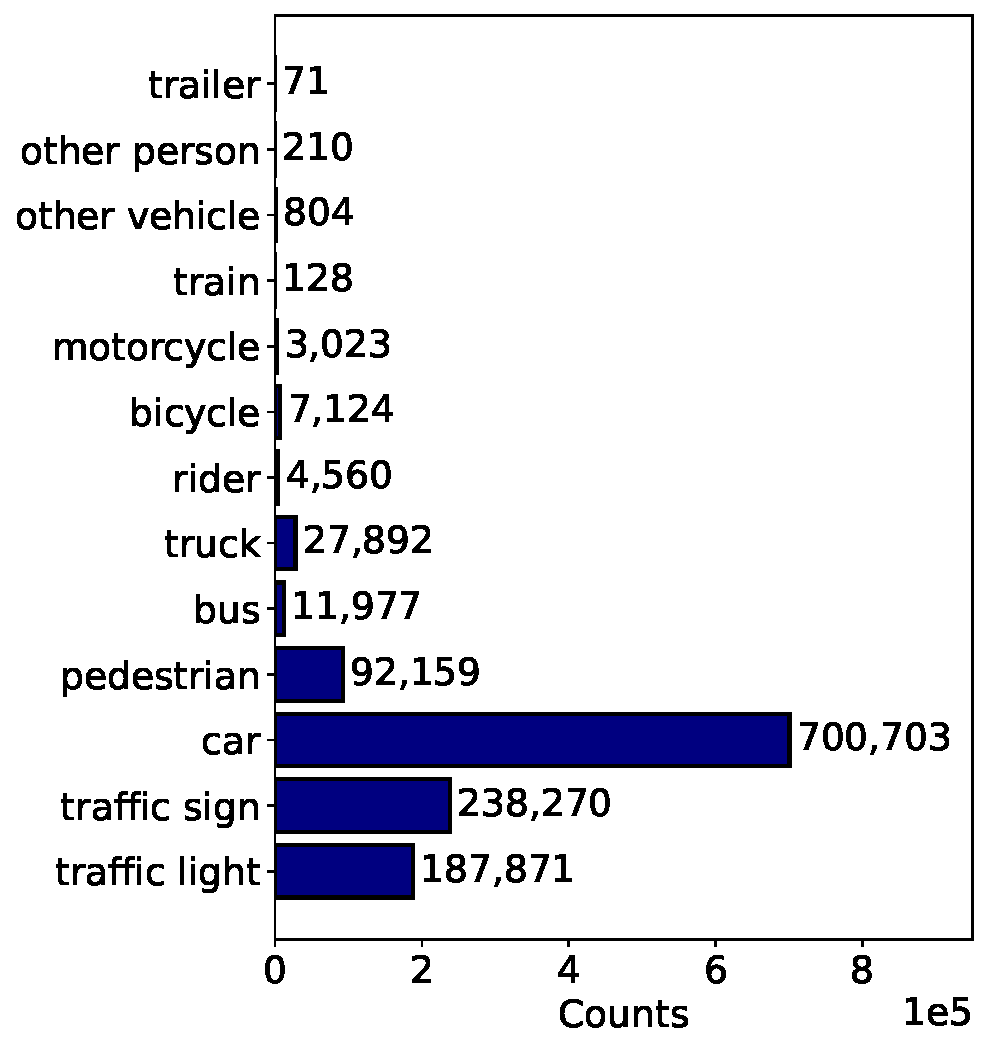
\includegraphics[width=\textwidth]{images/bdd100k/object_counts.pdf}
    \end{minipage}\hfill
    \begin{minipage}{0.49\textwidth}
        \centering
        \includegraphics[width=\textwidth]{images/bdd100k/frame_counts.pdf}
    \end{minipage}
    \caption{Distribution of classes in the training set of the BDD100k dataset.
    \textbf{Left}: Number of instances per class. 
    \textbf{Right}: Number of frames containing each class.
    }
    \label{fig:bdd100k_distribution}
\end{figure}

\subsection{Training on BDD100k}

\subsection{Experiments with GPT4-o}
In May 2024, OpenAI released GPT4-o, their multilingual, multimodal generative 
pre-trained transformer. Considering its powerful capability to describe general 
contexts in wide scenes, we decided to test the architecture to solve a problem 
similar to ours. Experiments were conducted on BDD100k dataset.

\subsubsection{Problem Definition}
We defined two groups of six images each. The first group consists of general 
driving scenarios that contain at least one person in each image. 
The second group, on the other hand, is still related to driving scenarios but 
does not contain any person. However, in most images of both groups there are 
some common objects, including cars, buildings, etc.
Then the model will be asked to evaluate a new, never seen, image and answer 
in which group it belongs.

Other experiments in the two groups were done, including asking the model which 
common targets are present in each group.

\subsubsection{Data Selections}
\setlength{\subfigwidth}{45mm}
\setlength{\horspace}{.3\textwidth}
\begin{figure}
    \centering
    \begin{tabular}{p{\horspace} p{\horspace} p{\horspace}}
    \begin{subfigure}[b]{\subfigwidth}
        \includegraphics[width=\subfigwidth]{images/gpt4/s1.jpg}
    \end{subfigure}
    \hfill &
    \begin{subfigure}[b]{\subfigwidth}
        \includegraphics[width=\subfigwidth]{images/gpt4/s2.jpg}
    \end{subfigure} 
    \hfill &
    \begin{subfigure}[b]{\subfigwidth}
        \includegraphics[width=\subfigwidth]{images/gpt4/s3.jpg}
    \end{subfigure} \\
    %
    \begin{subfigure}[b]{\subfigwidth}
        \includegraphics[width=\subfigwidth]{images/gpt4/s4.jpg}
    \end{subfigure}
    \hfill &
    \begin{subfigure}[b]{\subfigwidth}
        \includegraphics[width=\subfigwidth]{images/gpt4/s5.jpg}
    \end{subfigure} 
    \hfill &
    \begin{subfigure}[b]{\subfigwidth}
        \includegraphics[width=\subfigwidth]{images/gpt4/s6.jpg}
    \end{subfigure}
\end{tabular}
\caption{Group of safe images, there are no people in all the images.}
\label{fig:safe_group}
\end{figure}
%
\begin{figure}
    \centering
    \begin{tabular}{p{\horspace} p{\horspace} p{\horspace}}
    \begin{subfigure}[b]{\subfigwidth}
        \includegraphics[width=\subfigwidth]{images/gpt4/d1.jpg}
    \end{subfigure}
    \hfill &
    \begin{subfigure}[b]{\subfigwidth}
        \includegraphics[width=\subfigwidth]{images/gpt4/d2.jpg}
    \end{subfigure} 
    \hfill &
    \begin{subfigure}[b]{\subfigwidth}
        \includegraphics[width=\subfigwidth]{images/gpt4/d3.jpg}
    \end{subfigure} \\
    %
    \begin{subfigure}[b]{\subfigwidth}
        \includegraphics[width=\subfigwidth]{images/gpt4/d4.jpg}
    \end{subfigure}
    \hfill &
    \begin{subfigure}[b]{\subfigwidth}
        \includegraphics[width=\subfigwidth]{images/gpt4/d5.jpg}
    \end{subfigure} 
    \hfill &
    \begin{subfigure}[b]{\subfigwidth}
        \includegraphics[width=\subfigwidth]{images/gpt4/d6.jpg}
    \end{subfigure}
\end{tabular}
\caption{Group of dangerous images, there are some people in each image.}
\label{fig:dangerous_group}
\end{figure}
The first group of images is shown in Figure \ref{fig:safe_group}. It consists 
of six images that do not contain any person. In particular, in the first image 
on the top left there is the ego-vehicle in a highway with some other vehicles 
on the front. The second on the top-center represents a downtown scenario with 
some vehicles on the front. In the third image on top-right there is a vehicle 
on the front and many vehicles parked on both sides of the road. The fourth 
image on bottom-left represents the ego-vehicle driving on a road with a traffic 
divider and some cars parked on the right side. In the fifth image on the 
bottom-center there is a straight road with some vehicles on the front and tall 
buildings on the sides. The last image on the bottom-right represents a 
downtown scenario with some vehicles, including cars and a bus. There is 
actually an occluded person in the image, but it is almost not visible.

The second group of images is shown in Figure \ref{fig:dangerous_group}. 
In the first image on the top-left there are two cars in fron of the ego-vehicle, 
some cars parked on both sides and a pedestrian standing on the right side. There 
are also some other pedestrians far away on sidewalks, not much visible in the 
image.
The second image on the top-center represents a downtown scenario where some 
pedestrians are crossing the road. There is also a car partially visible on the 
right of the ego-vehicle. The environment is characterized by tall buildings.
The third image on the top-right represents a downtown scenario with some 
empty crosswalks but many pedestrians on sidewalks. There are also some cars 
driving on the main road.
The fourth image on the bottom-left represents a night downtown scenario with a 
taxi in front of the ego-vehicle and group of pedestrians on the left sidewalk 
and far away, where there are crosswalks and red traffic lights.
In the fifth image, bottom-center, there is a line of cars in front of the 
ego-vehicle, some cars parked on the left side, and a pedestrian standing on the 
left sidewalk.
The last image on the bottom-right represents a main road with some vehicles 
parked on both sides, some others driving, and a person standing on the right 
side of the road.

Considering the dangerous scenarios, some specific cases were carefully selected,
especially with people partially visible, in the corners of the images, and 
on the background. On the other hand, in both groups there are many vehicles, both 
in foreground and background, that contribute to add noise to the data to 
classify.
This decision represents a further challenge for the model to 
isolate the right group of pixels.

\subsubsection{Common Features Extraction}
The first experiment consists of showing the model the two groups of images, 
without explicitly explaining the difference between them. The model is asked 
to describe the common targets in each group. The question-answer pairs are 
shown below:
%
{\fontfamily{cmr}\selectfont
\begin{description}
    \item[Q:] What common targets do all the images have?
    Do not list a target if it is not inside all the images. 
    (\emph{showing the dangerous images})
    \item[A:] Cars, roads, \hl{people}, sky.
    \item[Q:] What common targets do all the images have?
    Do not list a target if it is not inside all the images. 
    (\emph{showing the safe images})
    \item[A:] Road, \hl{other vehicles}, sorrounding environment.    
\end{description}
}
It is possible to notice that for the dangerous images the model correctly 
detects also people as common targets. Moreover, vehicles are shown in both 
groups, and the model is able to distinguish them as common targets correctly.
This means that the model is able to extract the common noise in both groups 
(the presence of cars, that usually occupy many pixels with respect to people), 
but at the same time it is able to extract features of people related to the 
dangerous group.

This is a promising result, considering that GPT4 is a pretrained model on 
general multimodal data, and not specifically on driving scenarios. 
However, it has over 174 billion parameters, and that is why it is capable to 
generalize in many different contexts. Using a vision transformer architecture 
for specific tasks, like driving scenarios, with much less parameters, could 
still lead to good results.

\subsubsection{Grouping and Classification}
\setlength{\subfigwidth}{45mm}
\setlength{\horspace}{.3\textwidth}
\begin{figure}
    \centering
    \begin{tabular}{p{\horspace} p{\horspace}}
    \begin{subfigure}[b]{\subfigwidth}
        \includegraphics[width=\subfigwidth]{images/gpt4/s1.jpg}
    \end{subfigure}
    \hfill &
    \begin{subfigure}[b]{\subfigwidth}
        \includegraphics[width=\subfigwidth]{images/gpt4/s2.jpg}
    \end{subfigure} \\
    %
    \begin{subfigure}[b]{\subfigwidth}
        \includegraphics[width=\subfigwidth]{images/gpt4/s3.jpg}
    \end{subfigure}
    \hfill &
    \begin{subfigure}[b]{\subfigwidth}
        \includegraphics[width=\subfigwidth]{images/gpt4/s5.jpg}
    \end{subfigure}
\end{tabular}
\caption{Group of safe images, there are no people in all the images.}
\label{fig:sub_dangerous_group}
\end{figure}
%
\begin{figure}
    \centering
    \begin{tabular}{p{\horspace} p{\horspace}}
    \begin{subfigure}[b]{\subfigwidth}
        \includegraphics[width=\subfigwidth]{images/gpt4/d2.jpg}
    \end{subfigure}
    \hfill &
    \begin{subfigure}[b]{\subfigwidth}
        \includegraphics[width=\subfigwidth]{images/gpt4/d5.jpg}
    \end{subfigure} \\
    %
    \begin{subfigure}[b]{\subfigwidth}
        \includegraphics[width=\subfigwidth]{images/gpt4/d7.jpg}
    \end{subfigure}
    \hfill &
    \begin{subfigure}[b]{\subfigwidth}
        \includegraphics[width=\subfigwidth]{images/gpt4/d6.jpg}
    \end{subfigure}
\end{tabular}
\caption{Group of safe images, there are no people in all the images.}
\label{fig:sub_safe_group}
\end{figure}
\begin{figure}
\centering
\includegraphics[width=\subfigwidth]{images/gpt4/d1.jpg}
\caption{Test image}
\label{fig:test_image}
\end{figure}

In this experiment we only showed the model the two groups of images, without 
asking to extract common targets. Then we show a new image and ask the model 
to classify it in the right group. The question-answer pairs are shown below:
{\fontfamily{cmr}\selectfont
\begin{description}
    \item[Q:] I will show you two groups of images. Then I will show you a test 
    image and you have to tell me what group it is related to. You have to 
    identify common features for each group to find the correct matching. Do not 
    output anything before I have finished, when I will tell you "predict this 
    image".
    \item[A:] Understood! I'm ready when you are to proceed with the image groups 
    and the test image.
    \item[Q:] This is the first group. (\emph{showing the first group of images})
    \item[A:] I've received the first group of images. Please show me the next group.
    \item[Q:] This is the second group. (\emph{showing the second group of images})
    \item[A:] I've received the second group of images. Please proceed with showing 
    the test image when you are ready.
    \item[Q:] This is the test image. (\emph{showing the test image})
    \item[A:] Based on the test image and comparing it to the two groups shown earlier:
    The test image features an urban setting with buildings lining the streets 
    and multiple vehicles on the road. It closely resembles the environment and 
    context of the images in the second group, which also depict urban settings 
    with buildings, streets, and a 
    \hl{visible presence of pedestrians} or traffic. 
    This environment is distinct from the first group, which primarily showed 
    roads in more open, less densely populated areas or showing less urban 
    characteristics. 
    Therefore, \hl{the test image belongs to the second group}.
\end{description}
}
Also in this experiment the model is able to correctly classify the test image 
in the right group. The model is able to give a detailed explanation of the 
features that are common in the test image and in the second group of images.
It is impressive that the model is capable to give such detailed explanations 
of contexts in images, considering that it is a general model and not specifically 
trained on driving scenarios.

%
% \chapter{Discussion}

\section{Classical Computer Vision-based Approach}

\section{Deep Learning-based Approach}
%
\chapter{Conclusions}
\label{chpt:conclusion}

\section{Traditional Computer Vision-based Approach}

\section{Deep Learning-based Approach}

\section{Future Work}
%
\begin{appendices}
    \chapter{Training Algorithms}
    \begin{algorithm}
        \nextfloat{\caption{Preprocessing of DR(eye)VE dataset}}
        \vspace{0.2cm}
        \DontPrintSemicolon
        \textit{trainSet, valSet, testSet, ulSet} $\gets$ \textbf{Dreyeve}(\textit{splitIdxs, resolution, fps})\;
        \textit{validator} $\gets$ \textbf{RetinaNet}(\,)\;
        \For{\textit{set} $\gets$ \{\textit{trainSet, valSet, testSet}\}}{
            \textit{labels} $\gets$ validator(\textit{set})\;
            \textit{set.labels} $\gets$ \textit{labels}\;
        }
        \textbf{save} \textit{trainSet, valSet, testSet, ulSet}\;
    \end{algorithm}
    \begin{algorithm}
        \nextfloat{\caption{Semi-supervised training with Meta-Pseudo Labels}}
        \vspace{0.2cm}
        \DontPrintSemicolon
        \textit{trainSet, valSet, testSet, ulSet} $\gets$ \textbf{load} data\;
        \textit{teacher} $\gets$ \textbf{ViT}(\textit{patch, depth, embedding, mlp, heads})\;
        \textit{student} $\gets$ \textbf{ViT}(\textit{patch, depth, embedding, mlp, heads})\;
        \While{$\text{training}$}{
            \textit{pseudoLabels} $\gets$ \textit{teacher}(\textit{ulSet})\;
            \text{train(\textit{student, ulSet, pseudoLabels})}\;
            \text{train(\textit{student, trainSet})}\;
            \text{train(\textit{teacher, trainSet})}\;
            \textit{S.metrics} $\gets$ \text{validate(\textit{student, valSet})}\;
            \textit{T.metrics} $\gets$ \text{validate(\textit{teacher, valSet})}\;
            \If {$\textit{S.metrics.accuracy}$ \text{is increased}}{
                \textbf{save} \textit{student}\;
            }
        }
    \end{algorithm}
    \begin{algorithm}
        \nextfloat{\caption{Update training set with $N$ wrong predictions}}
        \vspace{0.2cm}
        \DontPrintSemicolon
        \textit{trainSet} $\gets$ \textbf{load} \text{training set}\;
        \textit{model} $\gets$ \textbf{load} \text{trained model}\;
        \textit{validator} $\gets$ \textbf{RetinaNet}(\,)\;
        \textit{S.count, S.max} $\gets$ $0, \,N/2$\;
        \textit{D.count, D.max} $\gets$ $0, \,N/2$\;
        \For{sample $\gets$ \textit{ulSet}}{
            \If{(\textit{S.count = S.max}) \textbf{and} (\textit{D.count = D.max})}{
                \textbf{break}\;
            }
            \textit{label} $\gets$ \textit{validator}(\textit{sample})\;
            \textit{pred} $\gets$ \textit{model}(\textit{sample})\;
            \If{\textit{pred} $=$ \textit{label}}{
                \textbf{continue}\;
            }
            \If{(\textit{label=Safe}) \textbf{and} (\textit{S.count \textless S.max})}{
                \textit{trainSet}.append(\textit{sample, label})\;
                \textit{S.count} $\gets$ \textit{S.count} $+1$\;
            }
            \If{(\textit{label=Dangerous}) \textbf{and} (\textit{D.count \textless D.max})}{
                \textit{trainSet}.append(\textit{sample, label})\;
                \textit{D.count} $\gets$ \textit{D.count} $+1$\;
            }
            \If{\textbf{endof} \textit{ulSet}}{
                \textbf{break}\;
            }
        }
        \textbf{save} \textit{trainSet}\;
    \end{algorithm}

\chapter{Probabilistic Perspective of \ac{roc}}
\end{appendices}
%
\printbibliography
%
\end{document}